%\documentclass[twoside]{pwrthesis}
\documentclass[twoside]{iisthesis}
% ---
\usepackage{polski}
\usepackage[utf8]{inputenc}
\usepackage{amsmath}
\usepackage{tocloft}
\usepackage{listings}
\usepackage{algorithm}
\usepackage{algorithmic}
\usepackage{mathtools}
\usepackage{graphicx}
\usepackage[colorinlistoftodos]{todonotes}
\usepackage{url}
\usepackage{pgfplots, pgfplotstable}
\selectlanguage{polish}
% Dodane przeze mnie d
\usepackage{fancyvrb} % dla srodowiska Verbatim
\usepackage{color}
\usepackage{lscape}
\usepackage{subfig}
\usepackage{multirow}
\usepackage{float}

\hypersetup{
    colorlinks,
    linkcolor={black!50!black},
    citecolor={black!50!black},
    urlcolor={black!80!black}
}

\definecolor{gray}{rgb}{0.4,0.4,0.4}
\definecolor{darkblue}{rgb}{0.0,0.0,0.6}
\definecolor{cyan}{rgb}{0.0,0.6,0.6}

\lstset{
  basicstyle=\ttfamily,
  columns=fullflexible,
  showstringspaces=false,
  commentstyle=\color{gray}\upshape
}

\lstdefinelanguage{XML}
{
  morestring=[b]",
  morestring=[s]{>}{<},
  morecomment=[s]{<?}{?>},
  stringstyle=\color{black},
  identifierstyle=\color{darkblue},
  keywordstyle=\color{cyan},
  morekeywords={xmlns,version,type}% list your attributes here
}

\lstset{
  language=XML,
   literate={ć}{{\'c}}1
}
\renewcommand*{\lstlistingname}{Kod źródłowy}
% definicje kolorow
\definecolor{ciemnoSzary}{rgb}{0.15,0.15,0.15}
\definecolor{szary}{rgb}{0.5,0.5,0.5}
\definecolor{jasnoSzary}{rgb}{0.2,0.2,0.2}

% Konfiguracja verbatima
\fvset{
	frame=single,
	numbers=left,
	fontsize=\footnotesize,
	numbersep=12pt,
%	framerule=.5mm,
	rulecolor=\color{ciemnoSzary},
%	fillcolor=\color{jasnoSzary},
	framesep=4pt,
	stepnumber=1,
	numberblanklines=false,
	tabsize=2,
%	formatcom=\color{szary}
}
\newcommand{\listequationsname}{Spis wzorów}
\newcommand{\equationcaption}[1]{\begin{flushright}\emph{#1}\end{flushright}}
\newcommand{\rightcaption}[1]{\begin{flushright}\emph{#1}\end{flushright}}
\newlistof{myequations}{equ}{\listequationsname}
\newcommand{\myequations}[1]{%
\addcontentsline{equ}{myequations}{\protect\numberline{\theequation}#1}\par}

\newcommand{\listofmyalgorithmsname}{Spis algorytmów}
\newlistof{myalgorithm}{algo}{\listofmyalgorithmsname}
\newcommand{\myalgorithm}[1]{%
\addcontentsline{algo}{myalgorithm}{\protect\numberline{\thealgorithm}#1}\par}


\newcommand{\listofmyfiguresname}{Spis rysunków}
\newlistof{myfigure}{figu}{\listofmyfiguresname}
\newcommand{\myfigure}[1]{%
\addcontentsline{figu}{myfigure}{\protect\numberline{\thefigure}#1}\par}

\floatname{algorithm}{Algorytm}

\newtheorem{mydef}{Definicja}



\begin{document}


\newcommand{\resultChart}[7][140]{
\def\dataS{{#2}}
	\begin{figure}[H]
	
\centering

\begin{center}
\begin{tikzpicture}
 
\begin{axis}[
ybar,
bar width=20,
legend style={at={(0.5,-0.25)},
anchor=north,legend columns=-1},
ylabel={Wartość miary},
symbolic x coords={\dataS},
xtick=data,
height=  {#1},
width=0.8\textwidth,
ymin=0, ytick={0,0.5,1},
ymax=1.5,
nodes near coords,
nodes near coords align={vertical},
]
\addplot coordinates { (\dataS,{#3}) };
\addplot coordinates {(\dataS,{#4}) };
\addplot coordinates { (\dataS,{#5}) };
\legend{Recall,Precission,F1-Score}
\end{axis}
\end{tikzpicture}
\end{center}
\caption{{#6}}
\myfigure{{#6}}
\label{{#7}}
\end{figure}
}


\pgfkeys{/pgf/number format/use comma}
\pgfkeys{/pgf/number format/.cd, set thousands separator={}}%
\nocite{*}
\title{ Wielokryterialny problem rozmieszczenia zraszaczy wodnych na zadanej powierzchni }
\titleEN{ Multicriteria water sprinklers deployment problem on a given area}
\shortTitle{}
\author{Grzegorz Dziedzic}
\advisor{dr Mariusz Fraś}
\instituteLogo{logos/pwr}
\slowaKluczowe{optymalizacja wielokryterialna,\\ algorytmy genetyczne,\\zraszacze wodne}

\date{\number\the\year}

% Wstawienie abstractu pracy
	%\input {abstract}

\abstractSH{Niniejsza praca miała na celu opracowanie systemu wspomagania podejmowania decyzji w rozmieszczeniu zraszaczy wodnych na zadanej powierzchni oraz wybór i porównanie wielokryterialnych algorytmów genetycznych w kontekście wybranego problemu.}

\abstractPL{
Celem niniejszej pracy było rozwiązanie wielokryterialnego problemu rozmieszczenia zraszaczy wodnych na zadanej powierzchni poprzez opracowanie systemu wspomagania podejmowania decyzji, a w szczególności wybór oraz porównanie wielokryterialnych algorytmów genetycznych w kontekście wybranego problemu. Jako cele procesu optymalizacji wybrano minimalizację obszaru nienawodnionego oraz minimalizacje kosztu zraszaczy, przy jednoczesnym uwzględnieniu minimalizacji nawodnienia obszaru poza wskazanym terenem oraz minimalizacji obszarów nawodnionych nadmiernie. Praca została podzielona na kilka części. Pierwszą z nich stanowi wprowadzenie w tematykę problemu, dokładniejszy opis rozwiązywanego problemu, przegląd literatura oraz definicja celu pracy. Kolejny rozdział jest opisem opracowanego modelu matematycznego, na którym swoje działanie opierają zaimplementowane algorytmy. W następnym rozdziale zdefiniowane są pojęcie optymalizacji oraz różnice pomiędzy optymalizacją jednokryterialną i wielokryterialną. W kolejnym rozdziale dokładnie opisany został schemat działania algorytmu genetycznego. Dodatkowo przedstawiono dwa algorytmy wybrane do rozwiązania omawianego problemu - NSGA-II oraz SPEA. Następna część pracy stanowi opis rezultatów. Najpierw przedstawiono opracowany system wspomagania decyzji, następnie porównano ze sobą wybrane algorytmy genetyczne oraz podsumowane różnice pomiędzy nimi. Na końcu pracy znajduje się podsumowanie, w którym umieszczono ocenę wykonanej pracy oraz dalsze możliwości rozwoju i badań.
}
\abstractEN{
The purpose of this thesis was solution of the multicriteria water sprinklers deployment problem on a given area. It was done by designing a decision support system and especially by selection and comparison of multicriteria genetic algorithms in the context of defined problem. As the purpose of optimization process the following objectives were defined: minimization of the not irrigated area and minimization of the chosen sprinklers' total cost, with the simultaneous minimization of the irrigation of the area placed out of bounds of selected region and minimzation of over irrigated area. The thesis was divied into several parts. First of them is and introduction to the chosen problem. Moreover it contains precise description of the problem, review of the literature and the definition of purpose. Next chapter describes developed mathematical model, that chosen algorithms are based on. Next chapter presents the definition of optimization and shows differences between single criteria optimization and multicriteria optimization. Next one is a precise description of genetic algorithms. Moreover it shows two algorithms chosen for solving defined problem - NSGA-II and SPEA. Next part of this thesis is a reflection of work that has been done. At first it shows designed decision support system. Then it presents the results of comparison made between chosen algorithms and summary of the their differences. At the end is a summary, where critical evaluation and further possibilites for development and analysis are placed.
}

\maketitle

\textpages


\graphicspath{ {img/} }
\DeclareGraphicsExtensions{.pdf,.png,.jpg}
\chapter{Wstęp}
\section{Wprowadzenie}
Odpowiednie nawodnienie jest jedną z podstawowych czynności pielęgnacyjnych ogrodu. Gdy właściciel dysponuje odpowiednim budżetem najlepszym rozwiązaniem będzie dla niego inwestycja w automatyczny system nawadniania. System taki składa się z zraszaczy wodnych, rur pomiędzy nimi oraz systemu sterowania. Takie rozwiązanie pozwala zaoszczędzić czas tracony na ręcznym podlewaniu ogrodu oraz zapewnia równomierne nawodnienie na całej ustalonej powierzchni. Jednym z głównych problemów koniecznych do rozwiązania podczas instalacji takiego systemu jest odpowiednie rozmieszczenie poszczególnych zraszaczy. Te najczęściej znajdują się pod ziemią oraz posiadają wynurzalną głowicę. Z tego powodu raz zainstalowany zraszacz najczęściej zostaje na swoim miejscu, aż do momentu wymiany całej instalacji wodnej. Biorąc to pod uwagę rozmieszczenie zraszaczy powinno być dobrze przemyślane już podczas etapu projektowania systemu nawadniania. Projektując taki system należy przyjąć jako cel nawodnienie całości wskazanego obszaru jak najmniejszym kosztem przy przestrzeganiu wskazanych przez właściciela ograniczeń.

Proces projektowania sieci zraszaczy może być żmudny oraz długotrwały, biorąc pod uwagę różnorodność sprzętu dostępnego na rynku czy chociażby nieregularność powierzchni, która ma zostać nawodniona. W Internecie można znaleźć mnóstwo poradników traktujących o tym jak samemu zaprojektować taki system nawadniania. Poradniki te jako główne narzędzia pracy polecają jednak kartkę papieru, ołówek oraz dużą ilość wolnego czasu, co już na wstępie może zniechęcać właścicieli ogrodów. Ewidentnie brakuje rozwiązań, które mogłyby ten proces zautomatyzować oraz ułatwić.
 
Z pomocą może przyjść jedna z gałęzi matematyki oraz informatyki, która obecna jest wokół nas na każdym kroku. Mowa tutaj o optymalizacji. Czym dokładnie jest optymalizacja zostanie opisane później. W tym momencie ważne natomiast jest to, że sformułowany powyżej scenariusz idealnie wpasowuje się w obszar problemów, których rozwiązania obejmują procesy optymalizacyjne. Jednym z najczęściej używanych narzędzi do rozwiązywania skomplikowanych problemów optymalizacyjnych stały się algorytmy genetyczne, opierające swoje działanie na procesach zachodzących w przyrodzie.

Praca ta będzie skupiać się na zautomatyzowaniu oraz ułatwieniu procesu projektowania systemu nawadniania ogrodu. Zostanie to zrealizowane poprzez implementację systemu wspomagania decyzji w formie aplikacji webowej, która pozwoli użytkownikowi na wczytanie planu swojego ogrodu, zaznaczenie obszaru, który ma zostać nawodniony oraz jako rezultat zwróci kilka wariantów rozmieszczenie zraszaczy wodnych oraz połączeń między nimi wraz z dokładną listą wykorzystanych elementów.

Problem optymalizacyjny wynikający z zdefiniowanego problemu zostanie rozwiązany za pomocą wielokryterialnego algorytmu genetycznego. Aby wybrać najlepszy wariant w pracy zostaną porównane dwa takie algorytmy: NSGA-II oraz SPEA. Na podstawie przeprowadzonych badań wybrany zostanie algorytm lepiej nadający się do zastosowania w opracowanym systemie wspomagania decyzji.
\section{Problem nawodnienia obszaru}
Jednym z podstawowych problemów z jakim spotykają się właściciele dużych oraz reprezentacyjnych ogrodów jest instalacja odpowiedniego systemu nawadniania. System taki jest potrzebny w celu utrzymania roślin znajdujących się na określonym terenie w odpowiedniej kondycji przy jednoczesnej automatyzacji całego procesu. System taki mogą zaprojektować oraz zainstalować sami albo zlecić to zadanie firmie zajmującej się takimi właśnie systemami.

Jest kilka szczególnie ważnych elementów, na które należy zwrócić uwagę projektując taki system \cite{irrigation_plan}:\\
\begin{itemize}
	\item Odpowiedni pomiar terenu, który ma zostać nawodniony.
	\item Wzięcie pod uwagę ukształtowania terenu.
	\item Obliczenie potrzebnego ciśnienia wody.
	\item Wybór i rozmieszczenie zraszaczy.
	\item Wybór i poprowadzenie rur.
	\item Umiejscowienie zaworów.\\
\end{itemize}
Wszystkie wymienione powyżej cechy znacząca wpływają na cenę, jakość oraz wydajność zaprojektowanego systemu.

W tej pracy skupiono się na dwóch z powyższych punktów: wyborze i rozmieszczeniu zraszaczy oraz poprowadzeniu rur.

Jak zostało wspomniane we wprowadzeniu, w systemach nawadniania najczęściej korzysta się ze zraszaczy wynurzalnych, a więc znajdujących się pod ziemią. Zmiana ułożenia sieci takich zraszaczy jest skomplikowana oraz niemożliwa bez przekopywania terenu pod którym znajduje się cała instalacja. Z tego względu układ zainstalowanych zraszaczy powinien być dobrze zaplanowany oraz przemyślany.

Pierwszym celem procesu projektowania powinno być takie rozmieszczenie zraszaczy, aby te były w stanie nawodnić cały wyznaczony teren przy jednoczesnym omijaniu obszarów, które nie powinny być podlane, jak na przykład budynki mieszkalne.

Kolejnym etapem staje się odpowiedni dobór mocy poszczególnych zraszaczy, a więc dystansu na jaki rozrzucają wodę. Po pierwsze eliminuje to problem nadmiernego nawodnienia danego obszaru. Po drugie minimalizuje koszty całej instalacji oraz jej utrzymania. Należy tutaj pamiętać, że im większy jest zasięg danego zraszacza tym wymaga większego ciśnienia co z kolei prowadzi do większego zapotrzebowania na wodę, a więc większych kosztów. Należy tutaj dodać również, że cena samego zraszacza jest zazwyczaj uzależniona od maksymalnej mocy danego modelu. Im ta jest większa tym więcej dany zraszacz będzie kosztował. Poprzez optymalizację doboru mocy każdego zraszacza z sieci minimalizuje się obszary nadmierne nawodnione oraz koszt całego systemu.

Kolejnym elementem jest odpowiednie poprowadzenie rur. Należy tutaj skupić się na dwóch elementach. Odpowiedniej średnicy wybranych rur oraz właściwym poprowadzeniu pomiędzy zainstalowanymi zraszaczami. Dobór średnicy odpowiada za ciśnienie wody dostarczanej do głowic. Niewystarczające ciśnienie sprawi, że zraszacz nie będzie mógł rozrzucać wody na wymaganym dystansie. Odpowiednie poprowadzenie rur z kolei pomaga zminimalizować koszty potrzebne do instalacji samych rur oraz połączeń pomiędzy nimi.

\section{Przegląd literatury}
Do tej pory problem nawodnienia danego obszaru nie był przedstawiany w literaturze w sposób zaproponowany w tej pracy. Istnieją jednak publikacje poruszające bardziej ogólny problem pokrycia terenu, w który dobrze wpasowuje się sformułowany problem.

W \cite{sensors} autorzy zajmują się problemem pokrycia danego obszaru w bezprzewodowych sieciach sensorów ze zmiennym zasięgiem. Sensor jest zdefiniowany jako okrąg o określonym zasięgu oraz współrzędnych środka. Na obszar mający zostać pokryty nakładana jest siatka składająca się z określonej liczby kwadratów. Sensor może zostać ulokowany w środku każdego takiego kwadratu. Autorzy w swojej pracy określili trzy kryteria względem których znalezione rozwiązania są oceniane. Są to:\\
\begin{enumerate}
	\item Stopień pokrycia terenu.
	\item Koszt rozmieszczonych sensorów.
	\item Koszt energetyczny rozmieszczonych sensorów.\\
\end{enumerate}
Jak widać problem przedstawiony w publikacji jest problemem wielokryterialnym. W celu rozwiązania przedstawionego problemu autorzy zdecydowali się na wykorzystanie algorytmu genetycznego NSGA-II.

W zaprezentowanych rezultatach autorzy zaczynali symulacje losowo rozmieszczając 500 sensorów. W 800. pokoleniu algorytm znalazł rozwiązanie składające się z 9 sensorów pokrywających 100\% wyznaczonego terenu oraz charakteryzujące się kosztem energetycznym na poziomie 0.576 (6-krotna poprawa względem 100. pokolenia).

Przedstawione wyniki są dowodem na odpowiednie podejście autorów do wielokryterialnego problemu pokrycia terenu. Do optymalizacji rozmieszczenia zraszaczy wodnych wykorzystano zmodyfikowany model matematyczny opisany w przedstawionej publikacji oraz wzorowano się na sposobie reprezentacji osobników w wykorzystanym algorytmie genetycznym.

Również na podstawie powyższej pracy zdecydowano, że do rozwiązania wielokryterialnego problemu pokrycia terenu dobrze sprawdza się wykorzystanie algorytmów genetycznych. W celu wyboru najlepszego algorytmu potrzebne były jednak badania oraz metryki definiujące jakość rozwiązań wygenerowanych przez poszczególne algorytmy.

Autorzy \cite{comparison_deb} skupiają się na porównaniu kilku wielokryterialnych algorytmów genetycznych. Do porównań wybrali sześć funkcji testowych. Ponadto autorzy zdefiniowali trzy metryki służące do oceny znalezionych rozwiązań oraz skonstruowali ranking obrazujący jakość działania każdego z wybranych algorytmów.

Kolejną pracą skupiającą się na porównaniu algorytmów genetycznych jest \cite{comparison_2}. W tej konkretnej publikacji autorzy porównują ze sobą dwa algorytmy: NSGA-II oraz OMOPSO. W pracy zdefiniowano trzy przypadki testowe oraz pięć metryk służących do ewaluacji znalezionych przez algorytmy rozwiązań.

Na podstawie dwóch powyższych prac wybrano dwa algorytmy wykorzystane do rozwiązania problemu zdefiniowanego w pracy (NSGA-II, SPEA) oraz zdefiniowano metryki służące do porównania rozwiązań generowanych przez wybrane algorytmy.

Kolejnym elementem był wybór odpowiedniego sposobu na poprowadzenie połączeń wodnych pomiędzy rozmieszczonymi zraszaczami.

W pracy \cite{pipes} autor skupia się na problemie minimalizacji wielkości systemu rur wodnych miasta Agric Nsima. Jest to motywowane zwiększającą się populacją, a tym samym zapotrzebowaniem na wodę. Autor poprzez rozwiązanie przedstawionego problemu chce zredukować koszty konieczne do funkcjonowania oraz utrzymania takiego systemu.

Autor w swojej pracy sugeruje, że najlepszym rozwiązaniem okazał się algorytm Prima, służący do znajdowania minimalnego drzewa rozpinającego grafu. Do poprowadzenia rur pomiędzy rozmieszczonymi zraszaczami zdecydowano na wykorzystanie proponowanego przez autora rozwiązania.

\section{Cel pracy}
Celem pracy jest opracowanie informatycznego systemu wspomagania podejmowania decyzji w rozmieszczeniu zraszaczy wodnych oraz połączeń pomiędzy nimi zadanej powierzchni, a w szczególności zaproponowanie oraz przebadanie wielokryterialnych algorytmów genetycznych w kontekście następujących kryteriów:\\
\begin{enumerate}
	\item Minimalizacja obszaru nienawodnionego.
	\item Minimalizacja kosztu wykorzystanych zraszaczy wodnych\\
\end{enumerate}
, przy zdefiniowanych ograniczeniach wymuszających minimalizację nawodnienia obszaru znajdującego się poza wyznaczonym terenem oraz minimalizację wielkości obszarów nawodnionych nadmiernie.

\section{Opis pracy}
W kolejnych rozdziałach opisane będą poszczególne zagadnienia związane z realizacją celu pracy. Na samym początku sformułowany zostanie model matematyczny opisujący rozwiązywany problem. Rozdział ten zawierał będzie dokładny opis podejścia do danego zagadnienia wraz z opisem wzorów matematycznych wykorzystanych do zdefiniowania poszczególnych funkcji celu. Następnie wyjaśnione zostaną pojęcia optymalizacji, optymalizacji jednokryterialnej oraz optymalizacji wielokryterialnej, czyli zagadnienia na których bazuje cała praca. W kolejnym rozdziale przedstawione zostaną algorytmy genetyczne, zarówno te w wersji podstawowej jak i wielokryterialnej wraz z ich wybranymi wersjami, tak aby przybliżyć czytelnikowi w jaki sposób ona działają oraz dlaczego są używane. Kolejne rozdziały będą już odzwierciedleniem wykonanej pracy i dokładnym opisem przyjętego sposobu realizacji zadania. Najpierw dokładnie opisany zostanie opracowany system wspomagania decyzji. Wymienione zostaną technologie użyte do implementacji oraz przykładowy scenariusz interakcji użytkownika z systemem wraz z zrzutami ekranu prezentującymi poszczególne widoki aplikacji. W kolejnym rozdziale zaprezentowane zostaną badania mające na celu porównanie wybranych algorytmów genetycznych. Na samym początku przedstawione zostaną cel oraz plan badań. Następnie zaprezentowane zostaną rezultaty procesu strojenia algorytmów. Kolejnym punktem będzie już prezentacja rezultatów badań oraz ich analiza wraz z podsumowaniem. Na końcu pracy znajdzie się ocena przedstawionego systemu wspomagania decyzji, argumenty za oraz przeciw używaniem algorytmów genetycznych w takich systemach oraz propozycje dalszego rozwoju systemu oraz prowadzenia badań.

\chapter{Model matematyczny}
Załóżmy, że $P$ jest wielokątem odwzorowującym kształt terenu, który ma zostać nawodniony. Poprzez opisanie danego wielokąta prostokątem otrzymujemy teren roboczy. Szerokość i wysokość tego terenu są dodatkowo powiększone o największy możliwy zasięg zraszaczy, tak aby umożliwić odpowiednie sprawdzenie stopnia naruszenia ograniczeń, o których mowa później. $A$ jest dodatkowo podzielony na $m \times n$ kwadratów tworząc macierz $M$ przedstawioną na rysunku \eqref{fig:matrix_m}. Każdy element macierzy może przyjmować wartości od 0 do $ms$, gdzie $ms$ jest maksymalną liczbą zraszaczy. Wartość 0 oznacza, że dany kwadrat nie został podlany. Wartość większa od 0 mówi o tym przez ile zraszaczy dany obszar został nawodniony.

\begin{figure}[!htb]
	\makebox[\textwidth]{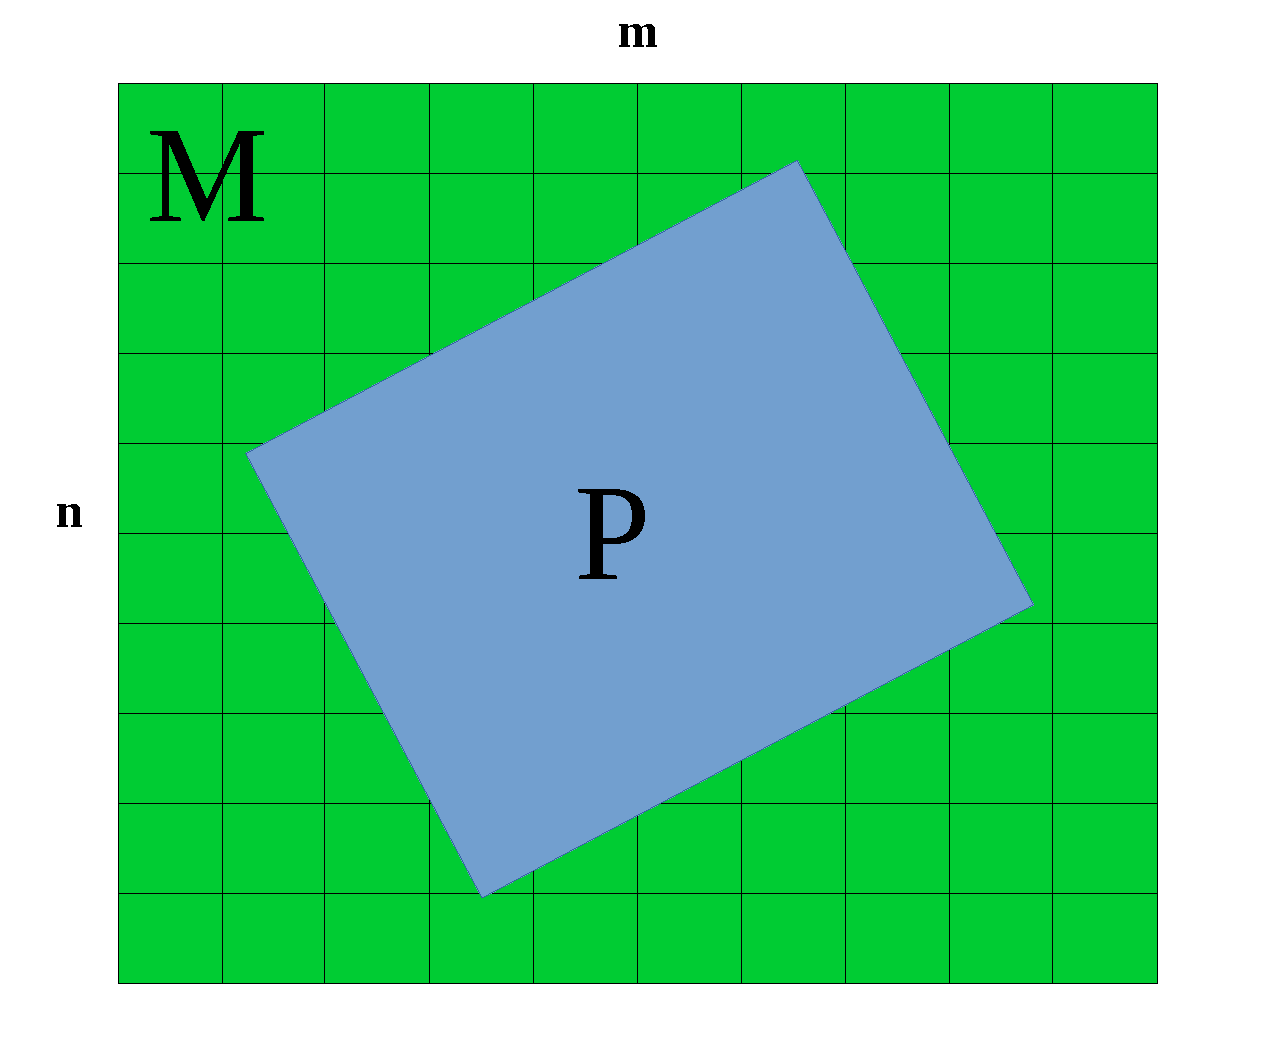
\includegraphics[ clip, scale=0.5]{mandf}}
	\centering
	\caption{Teren $P$ mający zostać podlany oraz macierz $M$.}
	\label{fig:matrix_m}
\end{figure}
Załóżmy, że $p(x,y)$ jest funkcją mówiącą o tym czy punkt o współrzędnych $(x, y)$ znajduje się wewnątrz $P$. Jeśli $p = 0$ punkt należy do $P$, w przeciwnym wypadku $p=1$. Zraszacz jest definiowany jako okrąg reprezentowany przez promień $r_{i}$, współrzędne środka $(x_i, y_i)$ oraz konkretny model $t_{i}$. Środek każdego zraszacza musi zawierać się w $P$, czyli $p(x_{i}, y_{i}) = 0$.

Kwadrat o współrzędnych $(x,y)$ jest nawodniony jeśli znajduje się w zasięgu zraszacza. Jest to wyrażone funkcją \eqref{eq:irrigated}.
\begin{equation}\label{eq:irrigated}
	is\_irr(x, y, s_{i}) = \begin{cases}
							1,& \text{jeśli } (x - x_{i})^{2} + (y - y_{i})^2 \leq r_{i}^{2}\\
							0,& w.p.p
						  \end{cases}
\end{equation}
, gdzie $x$ oraz $y$ oznaczają współrzędne środka kwadratu; $s_{i}$ jest konkretnym zraszaczem; $x_{i}, y_{i}$ oznaczają współrzędne zraszacza $s_{i}$; $r_{i}$ jest liczba wyrażającą zasięg zraszacza.\\\\
Załóżmy, że $S$ jest zbiorem wszystkich rozmieszczonych zraszaczy. Wtedy dany kwadrat jest nawodniony jeśli znajduje się w zasięgu przynajmniej jednego zraszacza ze zbioru $S$ \eqref{eq:irrigated_total}.
\begin{equation}\label{eq:irrigated_total}
	irr(x, y, S) = \begin{cases}
				   	1,& \text{jeśli } \sum_{i=1}^{S} is\_irr(x,y,s_{i}) > 0 \\
				   	0,& w.p.p			   	
				   \end{cases}
\end{equation}
Generalnie poprzez wielkość obszaru nienawodnionego rozumie się jako różnicę pomiędzy liczbą wszystkich elementów macierzy $M$ należących do $P$, a liczbą nawodnionych elementów tej macierzy należących do $P$ \eqref{eq:simple_f1}.
\begin{equation}\label{eq:simple_f1}
	F_{0}(S) = \sum_{m=1}^{M}\sum_{n=1}^{N} p(m,n)(1 - irr(m,n,S))
\end{equation}
, gdzie $F_{0}$ jest dodatkową funkcją pomagającą zobrazować podejście do problemu. Im wartość funkcji $F_{0}$ jest mniejsza tym obszar nienawodniony jest mniejszy, a więc rozwiązanie jest lepsze. $F_{0} = $ jest rozwiązaniem idealnym z perspektywy kryterium nawodnienia.


Na podstawie funkcji obrazującej wielkość obszaru nienawodnionego \eqref{eq:simple_f1} sformułowano bardziej szczegółową funkcję biorącą pod uwagę stopień naruszenia ograniczeń. Zostały one zdefiniowane w celu minimalizacji nawodnienia obszaru znajdującego się poza wyznaczonym terenem \eqref{eq:constraint_out_of_bounds} oraz minimalizacji wielkości obszarów nawodnionych nadmiernie \eqref{eq:constraint_overrirr}. Wpływ ograniczeń został wprowadzony w formie funkcji kary sumującej stopień ich naruszenia \eqref{eq:constraint_sum}.

\begin{equation}\label{eq:constraint_out_of_bounds}
	\omega_{1}(S) = \dfrac{\sum_{m=1}^{M}\sum_{n=1}^{N} (1 - p(m,n)) \cdot irr(m,n,S) \cdot \beta}{\sum_{m=1}^{M}\sum_{n=1}^{N} p(m,n)}
\end{equation}
, gdzie $\beta$ jest współczynnikiem mówiącym o mocy danego ograniczenia. Domyślnie $\beta=100$.\\
\begin{equation}\label{eq:constraint_overrirr}
	\omega_{2}(S) = \dfrac{\sum_{m=1}^{M}\sum_{n=1}^{N} p(m,n) \cdot ovrirr(m,n,S) \cdot \beta}{\sum_{m=1}^{M}\sum_{n=1}^{N} p(m,n)}
\end{equation}
, gdzie $ovrirr(m,n,S)$ jest funkcją mówiącą czy dany obszar został nadmiernie nawodniony \eqref{eq:is_overirrigated_func}.\\
\begin{equation}\label{eq:is_overirrigated_func}
	ovrirr(x,y,S) = \begin{cases}
				1,& \text{jeśli } \sum_{i=1}^{S} is\_irr(x,y,s_{i}) > 1 \\
				0,& w.p.p
			   \end{cases}
\end{equation}

\begin{equation}\label{eq:constraint_sum}
	\Omega(S) = \sum_{j = 1}^{J} \omega_{j}(S)
\end{equation}
, gdzie $J$ jest zbiorem wszystkich zdefiniowanych ograniczeń.\\

Po uwzględnieniu zdefiniowanych ograniczeń funkcja oceniająca wielkość obszaru nienawodnionego wygląda w sposób przedstawiony na równaniu \eqref{eq:f_one}.
\begin{equation}\label{eq:f_one}
F_{1}(S) = \sum_{m=1}^{M}\sum_{n=1}^{N} p(m,n) \cdot (1 - irr(m,n,S)) + \Omega(S)
\end{equation}

Jak zostało wspomniane wcześniej, każdy rozmieszczony zraszacz charakteryzowany jest przez konkretny model. Załóżmy, że $C(t_{i})$ jest funkcją zwracającą cenę rynkową dla danego modelu $t_i$. Wtedy całkowity koszt konkretnego rozwiązania jest zdefiniowany poprzez równanie \eqref{eq:f_two}.
\begin{equation}\label{eq:f_two}
	F_{2}(S) = \sum_{i=1}^{S} C(t_{i})
\end{equation}\\

Podsumowując celem zadania jest rozwiązanie problemu optymalizacyjnego sformułowanego w następujący sposób:\\

Dla danych $M, P, ms$ oraz z uwzględnieniem zdefiniowanych ograniczeń \eqref{eq:constraint_out_of_bounds}, \eqref{eq:constraint_overrirr} znajdź wektor $S^{*}$ minimalizujący wielkość obszaru nienawodnionego oraz minimalizujący koszt danego rozwiązania \eqref{eq:final_model}.
\begin{equation}\label{eq:final_model}
	\begin{split}
		min \text{  }&  F_{1}(S) = \sum_{m=1}^{M}\sum_{n=1}^{N} p(m,n) (1 - irr(m,n,S)) + \Omega(S)\\
		min \text{  }&	F_{2}(S) = \sum_{i=1}^{S} C(t_{i})
	\end{split}
\end{equation}

\chapter{Optymalizacja}
Optymalizacja jest procesem polegającym na wyznaczeniu najlepszego rozwiązania lub rozwiązań z punktu widzenia danego kryterium lub kryteriów \cite{wiki_optimization}. Procesy takie w w obecnym świecie obecne są wszędzie. Zaczynając od mechaniki, poprzez ekonomie, finanse, elektrykę po geofizykę czy modelowanie molekularne. Przykładem może być konieczność minimalizacji kosztów produkcji w fabryce, maksymalizacja prawdopodobieństwa zysku z przeprowadzanych transakcji czy chociażby znalezienie najbardziej odpowiadającego danej osobie modelu samochodu \cite{wiki_pl_optimization}.

W kolejnych podrozdziałach dokładnie opisane zostaną zagadanie powiązane kolejno z optymalizacją jednokryterialną oraz wielokryterialną.
\section{Optymalizacja jednokryterialna}
Optymalizacja jednokryterialna, jak wskazuje nazwa, odnosi się do problemów opisywanych za pomocą jednej funkcji celu. Przykładem może być tutaj problem spotykający ludzi wybierających się na wakacje, a więc poszukiwanie najlepszego hotelu w danym mieście. Załóżmy, że jedynym kryterium branym pod uwagę w trakcie szukania takiego hotel jest cena ze spędzoną noc. Przykładem będzie tutaj sytuacja przestawiona na rysuku \eqref{fig:opt_ex}. Jak łatwo zauważyć najtańszy jest hotel $A$. Można więc powiedzieć, że hotel $A$ jest rozwiązaniem przedstawionego problemu optymalizacyjnego. Patrząc na to z drugiej strony, możemy stwierdzić, że cena hotelu nie ma dla nas żadnego znaczenia, a zależy nam jedynie na tym aby ten znajdował się jak najbliżej morza. Przy takiej zmianie kryterium, zmienia się również rozwiązanie problemu. Najlepszy staje się hotel $E$, ponieważ to właśnie on znajduje się najbliższej morza.

Z matematycznego punktu widzenia rozwiązanie jednokryterialnego problemu optymalizacyjnego sprowadza się do znalezienia ekstremum  funkcji opisującej wybrane kryterium oceny \cite{wiki_pl_optimization}.
\begin{figure}[!htb]
	\makebox[\textwidth]{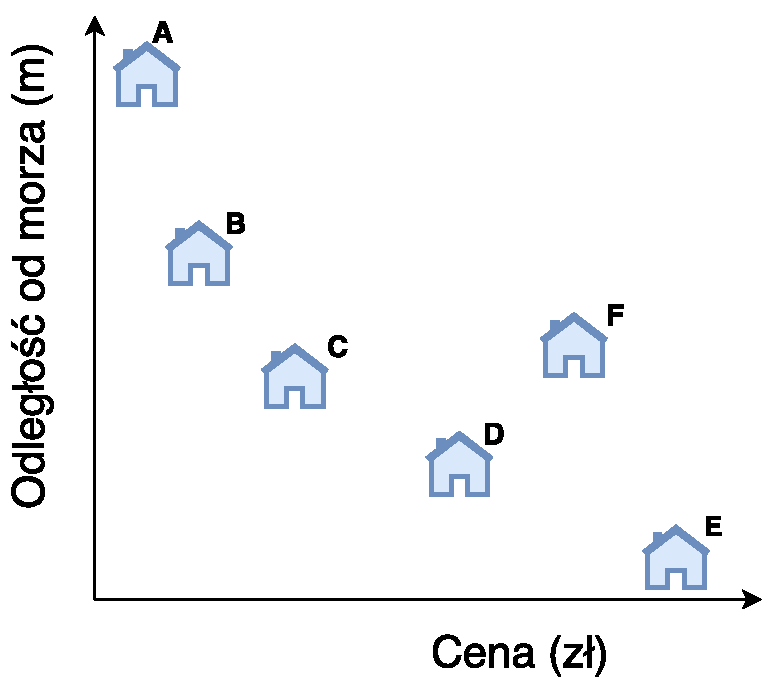
\includegraphics[ clip, scale=0.6]{opt_ex}}
	\centering
	\caption{Powiązanie pomiędzy ceną hotelu, a dystansem od morza}
	\label{fig:opt_ex}
\end{figure}
\section{Optymalizacja wielokryterialna}
Jeśli problem optymalizacyjny zawiera w sobie kilka funkcji celu, proces znajdowania optymalnego rozwiązania bądź rozwiązań nazywa się optymalizacją wielokryterialną. Zdecydowana większość realnych problemów jest właśnie przykładem wymagającym wykorzystania optymalizacji wielokryterialnej \cite{book}. W takich przypadkach nie można skupiać się jedynie na jednym kryterium, ponieważ pozostałe są równie ważne. Przykładem może być tutaj problem wyboru hotelu na wakacje, opisany w poprzednim podrozdziale. 

Załóżmy, że tym razem oba kryteria przedstawione na rysunku \eqref{fig:opt_ex} są dla nas tak samo ważne. Gdyby było inaczej i wszyscy kierowali by się jedynie ceną hotelu, wszyscy chcieliby mieszkać w hotelu $A$. Oczywiście w realnym świecie taka sytuacja nigdy nie będzie miała miejsca, ponieważ w większości przypadków proces decyzyjny nie jest taki prosty.

Jak możemy zauważyć do wyboru mamy 6 różnych hoteli. Każdy z nich charakteryzuje się ceną za jedną noc oraz odległością od morza wyrażoną w metrach. Do porównania wybierzmy dwa hotele: $D$ oraz $F$. Jak widać hotel $D$ jest zarówno tańszy jak i znajduje się bliżej morza w porównaniu do hotelu $F$. W tym przypadku decyzja o wyborze jest oczywista i jest nią hotel $D$. Sytuacja wygląda inaczej, gdy porównamy hotel $D$ z hotelem $C$. Hotel $D$ znajduję się bliżej plaży, natomiast jest również droższy od $C$. Które rozwiązanie w tej sytuacji będzie lepsze? To już zależy wyłącznie od preferencji konkretnej osoby. Nie da się bowiem stwierdzić, które z wybranych rozwiązań jest lepsze patrząc z perspektywy obu kryteriów. Z tego powodu problemy, w których występuje kilka kryteriów negatywnie na siebie wpływających, charakteryzują się posiadaniem wielu rozwiązań optymalnych \cite{book_ergot}.

\subsubsection{Dominacja}
Jednym z głównych pojęć, na których opiera się optymalizacja wielokryterialna jest pojęcie dominacji. Jednym z celów rozwiązywania problemów wielokryterialnych jest znalezienie rozwiązań niezdominowanych, co dokładniej wyjaśnione zostanie później. Koncept dominacji polega na porównywaniu ze sobą znalezionych rozwiązań przez pryzmat wszystkich określonych kryteriów oceny. Załóżmy, że $M$ określa liczbę kryteriów. Wtedy można powiedzieć, że rozwiązanie $A$ dominuje rozwiązanie $B$ jeśli \cite{book}:\\
\begin{enumerate}
	\item Dla każdego kryterium $m \in M$ rozwiązanie $A$ nie jest gorsze od $B$.
	\item Przynajmniej dla jednego kryterium $m \in M$ rozwiązanie $A$ jest lepsze od $B$.\\
\end{enumerate}
Korzystając z opisanego wcześniej przykładu hoteli, możemy zauważyć, że rozwiązanie $F$ jest zdominowane przez rozwiązanie $D$. Jest tak dlatego, że rozwiązanie $D$ jest pod względem każdego kryterium lepsze od rozwiązania $F$, a więc spełnione są wymienione powyżej warunki. Nie można tego samego powiedzieć, gdy do porównania użyjemy hotelu $A$ oraz $B$. Rozwiązanie $A$ nie spełnia pierwszego warunku - hotel jest położony dalej od morza.

\subsubsection{Optimum Pareto}
Rozwiązanie jest rozwiązaniem optymalnym w sensie Pareto, jeśli nie da się poprawić danego rozwiązania pod względem jednego kryterium, nie pogarszając jednocześnie oceny rozwiązania, patrząc z perspektywy pozostałych kryteriów \cite{wiki_pareto}. Spójrzmy na hotel $C$ z wykorzystywanego wcześniej przykładu oraz załóżmy, że jest to rozwiązanie optymalne w sensie Pareto. W takiej sytuacji nie da obniżyć się ceny za pobyt w hotelu bez zmiany jego lokalizacji, oddalającej go od plaży. Sytuacja wygląda identycznie w drugą stronę. Nie da się zmienić położenia hotelu na bliższe morzu, bez zwiększenia ceny za noc. Optimum Pareto jest więc kompromisem pomiędzy pomiędzy uwzględnianymi kryteriami.

Grupa rozwiązań optymalnych w sensie Pareto tworzy tzw. front lub zbiór Pareto. Rozwiązanie optymalne w sensie Pareto jest jednocześnie rozwiązaniem niezdominowanym, tak więc front Pareto jest również zbiorem rozwiązań niezdominowanych \cite{book}. Przykład takiego frontu, w postaci niebieskiej linii, został przestawiony na rysunku \eqref{fig:pareto_ex}. Rozwiązania (1-4) leżące na froncie są rozwiązaniami optymalnymi w sensie Pareto, które dominują pozostałe rozwiązania znajdujące się na rysunku.
\begin{figure}[!htb]
	\makebox[\textwidth]{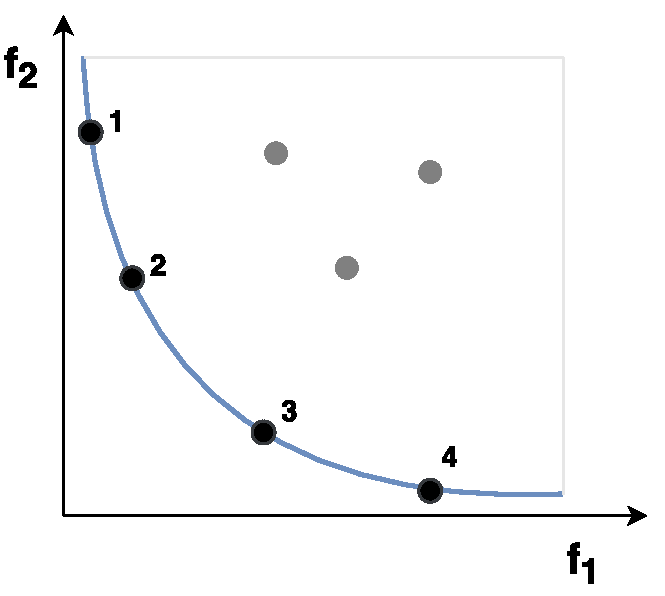
\includegraphics[ clip, scale=0.5]{pareto_ex}}
	\centering
	\caption{Front Pareto}
	\label{fig:pareto_ex}
\end{figure}

Przedstawiona powyżej definicja frontu Pareto może zostać wykorzystana w dwóch kontekstach: lokalnym oraz globalnym. Front Pareto w sensie globalnym jest zbiorem rozwiązań niezdominowanych w kontekście całej przestrzeni możliwych rozwiązań. Taki front nazywany jest również prawdziwym frontem Pareto \cite{book}. Lokalny front Pareto natomiast, jest grupą rozwiązań niezdominowanych ale tylko w określonym zakresie przestrzeni. Biorąc to pod uwagę dowolną grupę rozwiązań można podzielić na $n$ frontów, gdzie $n$ jest liczbą frontów potrzebnych do objęcia wszystkich rozwiązań z grupy. Zostało to zobrazowane na rysunku \eqref{fig:fronts_ex}. Liczby znajdujące się przy frontach oznaczają ich miejsce w hierarchii. Najlepszy front oznaczony jest liczbą 1, kolejny liczbą 2 itd.. Warto tutaj zauważyć, że rozwiązania znajdujące się na drugim froncie nie są niezdominowane w sensie globalnym (dominują je rozwiązania z frontu pierwszego). Są natomiast optymalne w sensie lokalnym, czyli po ograniczeniu przestrzeni rozwiązań do tych nieznajdujących się na pierwszym froncie.
\begin{figure}[!htb]
	\makebox[\textwidth]{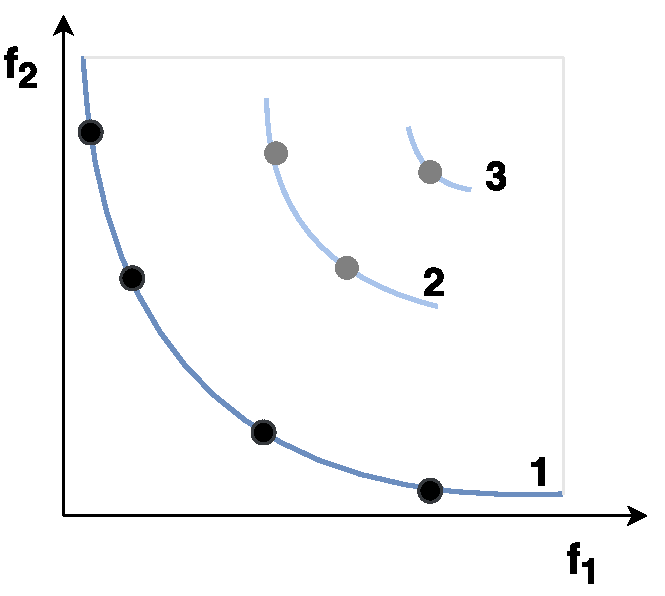
\includegraphics[ clip, scale=0.6]{fronts_ex}}
	\centering
	\caption{Lokalne fronty Pareto}
	\label{fig:fronts_ex}
\end{figure}
\subsubsection{Znajdowanie rozwiązań niezdominowanych}
Kolejnym ważnym zagadnieniem jest proces znajdowania rozwiązań niezdominowanych w danej grupie rozwiązań \cite{book}. Proces ten jest wykorzystywany w większości metod służących do optymalizacji wielokryterialnej, m.in. w wielokryterialnych algorytmach genetycznych opisanych w kolejnym rozdziale.

Istnieje wiele sposobów na posortowanie grupy ze względu na kryterium dominacji. Najprostszym z nich jest podejście iteracyjne. Polega ono na porównaniu danego rozwiązania $i$, z każdym innym rozwiązaniem. Jeśli rozwiązanie $i$ jest zdominowane przez jakiekolwiek inne rozwiązanie, znaczy to, że nie może zostać dodane do zbioru rozwiązań niezdominowanych. Generalnie dla danego zbioru rozwiązań $S$ o rozmiarze $N$, algorytm iteracyjny może zostać opisany następującymi krokami:\\

\begin{enumerate}
	\item Utwórz pusty zbiór rozwiązań niezdominowanych $P'$.
	\item Ustaw licznik $i = 0$.
	\item Dla każdego rozwiązania $j$, takiego że $j \neq i$, sprawdź czy rozwiązanie $j$ dominuje rozwiązanie $i$. Jeśli tak przejdź do punktu 5.
	\item Jeśli $j < N$, zwiększ licznik $j$ oraz przejdź do punktu 2. Jeśli $j = N$, dodaj rozwiązanie $i$ do zbioru rozwiązań niezdominowanych.
	\item Jeśli $i < N$, zwiększ licznik $i$ oraz przejdź do punktu 2. W innym wypadku $P'$ jest końcowym zbiorem rozwiązań niezdominowanych.\\
\end{enumerate}
Przedstawiony powyżej algorytm jest prosty ale też cechuje się dużą złożonością obliczeniową. Łatwo zauważyć, że złożoność punktu 3. w najgorszym przypadku wynosi $O(MN)$. Z racji tego, że punkt 4. rekursywnie wywołuje punkt 2, wymaga on złożoności obliczeniowej $O(MN^{2})$. Warto zauważyć, że jest to najgorszy możliwy przypadek, ponieważ w drugim kroku nie zawsze konieczne jest wykonanie wszystkich ($N-1$) porównań \cite{book}.

Lepszym rozwiązaniem jest zastosowanie efektywnej metody opracowanej przez Kunga wraz z innymi autorami (Kung et al.'s Efficient Method). Jak zostało wykazane metoda ta cechuje się złożonością obliczeniową $O(N(\log N)^{M-2})$ dla ponad trzech kryteriów oceny oraz $O(N\log N)$ dla dwóch i trzech kryteriów oceny \cite{kung}.

Pierwszym krokiem metody jest posortowanie grupy rozwiązań na podstawie wartości pierwszej funkcji oceny, w kolejności od najlepszego do najgorszego. Następnie grupę dzielona jest na połowę, tworząc dwie podgrupy: górną (T) oraz dolną (B). Sortowanie zapewniło, że rozwiązania z grupy T są lepsze od rozwiązań z grupy B z perspektywy pierwszego kryterium. Kolejnym krokiem jest porównywanie rozwiązań z dolnej grupy z rozwiązaniami z grupy górnej w kontekście dominacji. Rozwiązanie niezdominowane są przenoszone do górnej grupy. Operacje łączenia oraz porównania zaczynają być wykonywane, gdy w wyniki rekursywnego podziału grupy na dwie podgrupy, w danej podgrupie znajduje się jedynie jedno rozwiązanie. Przedstawiony proces może zostać zobrazowany w formie kodu głównej funkcji:
\lstset{
language=Python,
keywordstyle=\color{red}\ttfamily,
stringstyle=\color{black}\ttfamily,
frame=tb,
columns=fullflexible,
showstringspaces=false
}
\begin{lstlisting}[label=some-code,caption=Znajdowanie rozwiązań niezdominowanych]
def Front(P):
	if len(P) == 1:
		return P
	T = Front(P[:len(pop)/2])
	B = Front(P[len(pop)/2:])
	
	NotDominatedSolutions = []
	for B_Solution in B:
		NotDominated = True
		for T_Solution in T:
			if T_Solution.Dominates(B_Solution):
				NotDominated = False
				break
		if NotDominated:
			NotDominateSolutions.append(B_Solution)
	NotDominatedSolutions += T
	return NotDominatedSolutions
\end{lstlisting}
Kod został napisany w języku Python 2.7. Argumentem funkcji ($P$) jest posortowana lista rozwiązań.

Ze względu na najlepszą złożoność obliczeniową metoda opisana powyżej została zaimplementowana w wybranych algorytmach genetycznych.

\subsubsection{Sortowanie rozwiązań niezdominowanych}
Większość z metod służących do rozwiązywania problemów wielokryterialnych wykorzystuje koncept znajdowania zbioru rozwiązań niezdominowanych. Istnieją również algorytmy, w tym opisywany później NSGA-II, które wymagają podziału całej populacji na kolejne niezdominowane grupy (fronty) \cite{book}. W takim przypadku populacja jest przechowywana jako zbiór frontów ułożonych w kolejności od najlepszego (front pierwszy) do najgorszego.

Istnieje prosta procedura służąca do dzielenia całej populacji na poszczególne fronty \cite{nsga}. Wykorzystuje ona metody opisane w poprzedniej sekcji. Po znalezieniu pierwszego frontu, rozwiązania należącego do niego stają się tymczasowo ignorowane. Następnie procedura jest powtarzana, w celu znalezienia kolejnego frontu. Ponownie rozwiązania leżące na danym froncie są dodawane do grupy rozwiązań ignorowanych. Proces jest powtarzany, dopóki każde rozwiązanie z populacji nie jest przyporządkowane do odpowiedniego frontu.

\subsubsection{Cele optymalizacji wielokryterialnej}
Jak zostało wspomniane wcześniej rezultatem procesu optymalizacji wielokryterialnej, nie jest jedno rozwiązanie, lecz grupa rozwiązań. Grupę taką ocenia się z perspektywy dwóch kryteriów \cite{book}. Po pierwsze grupa ta powinna znajdować się jak najbliższej prawdziwego frontu Pareto. Rozwiązanie idealne odwzorowuje sytuację kiedy każde znalezione rozwiązanie jest optymalne w sensie Pareto. Po drugie znaleziona grupa powinna cechować się różnorodnością. Jest to ważne z perspektywy zachowania takiej samej wagi dla każdego ustalonego kryterium. Warto tutaj wspomnieć, że proces optymalizacji wielokryterialnej nie jest odpowiedzialny za wybór jednego konkretnego rozwiązania, które będzie najlepsze dla konkretnego użytkownika. Wynikiem takiej optymalizacji ma być natomiast zbiór równie dobrych rozwiązań, z których użytkownik będzie mógł wybrać najbardziej dla siebie odpowiednie. Im większa różnorodność rozwiązań tym więcej opcji do wyboru ma użytkownik.

Oba wymienione kryteria są tak samo ważne, dlatego algorytmy służące do optymalizacji wielokryterialnej powinny skupiać się na zaspokojeniu obu tych kryteriów w takim samym stopniu \cite{book}.

\chapter{Algorytmy genetyczne}
Problem rozmieszczenia zraszaczy opisany na wstępie pracy został rozwiązany przy użyciu algorytmów genetycznych. Są to algorytmy, których działanie oparte jest na tych samych zasadach na których odbywa się proces ewolucji zachodzący w naturze \cite{ga_book}. W tym rozdziale przedstawiony zostanie opis ogólny algorytmu genetycznego, jego powiązanie z procesami zachodzącymi w przyrodzie, schemat działania oraz dokładny opis wykorzystywanych operatorów: krzyżowania, selekcji oraz mutacji. Następnie przedstawiony zostanie koncept wielokryterialnych algorytmów genetycznych oraz opisane zostaną dwa algorytmy wykorzystane do rozwiązania przedstawionego wcześniej problemu: NSGA-II oraz SPEA. Następnie opisana zostanie konkretna implementacja zastosowana w celu rozwiązania problemu nawodnienia.

\section{Opis ogólny}
Algorytmy genetyczne są procedurami wykorzystywanymi do rozwiązywania problemów optymalizacyjnych, opartymi o genetykę oraz selekcję naturalną. Cały proces działania takiego algorytmu można porównywać do procesu ewolucji występującego w przyrodzie \cite{ga_book}. Obserwując taki proces można zauważyć, że najlepiej przystosowane osobniki mają największe szanse na reprodukcję, a więc przekazanie swojego DNA kolejnym pokoleniom. Dzieje się tak dlatego, że z punktu widzenia biologii najlepiej przystosowane osobniki to te najbardziej atrakcyjne dla potencjalnych partnerów oraz w przypadku zwierząt stadnych, te dominujące całą resztę, a więc mające pierwszeństwo jeśli chodzi o wybór partnerów, reprodukcję czy chociażby pożywianie się. Generalizując natura dąży do tego, aby do puli z której utworzone ma zostać kolejne pokolenie danej populacji trafiały jak najlepsze geny. Gdyby działo się inaczej żaden gatunek nie przetrwałby więcej niż kilkudziesięciu pokoleń.

Jak zostało wspomniane największe szanse na potomstwo mają osobniki najlepsze patrząc z perspektywy szansy na przetrwanie. Potomstwo par takich osobników powstaje na skutek procesu nazywanego krzyżowaniem. Krzyżowanie polega na łączeniu genów jednego osobnika z drugim, tworząc w ten sposób potomka, charakteryzującego się cechami zarówno pierwszego jak i drugiego rodzica. Oczywiście im lepiej rodzice danego osobnika byli przystosowani, tym większa szansa, że również i on będzie stał wysoko w hierarchii.

Kolejnym istotnym elementem w procesie ewolucji jest mutacja. Mutacja jest losowym procesem polegającym na zmianie fragmentu kodu DNA. Poprzez taką zmianę osobnik staje się jeszcze lepiej lub gorzej przystosowany. W pierwszym przypadku jego szanse na reprodukcję wzrastają, więc jest większe prawdopodobieństwo, że zmiana wprowadzona przez mutację zostanie przekazana dalej. W drugim przypadku linia osobników ze zmienionym DNA prawdopodobnie wygaśnie zdecydowanie szybciej niż w przypadku pierwszym.

Podsumowując, proces ewolucji złożony jest z trzech elementów: selekcji, krzyżowania oraz mutacji \cite{ga_book}. Na tych samych operacjach opiera się działanie algorytmu genetycznego. W kontekście algorytmu są one nazywane operatorami genetycznymi. Na rysunku \eqref{fig:ga_sequence} przedstawiony został ogólny schemat działania takiego algorytmu.
\begin{figure}[!htb]
	\makebox[\textwidth]{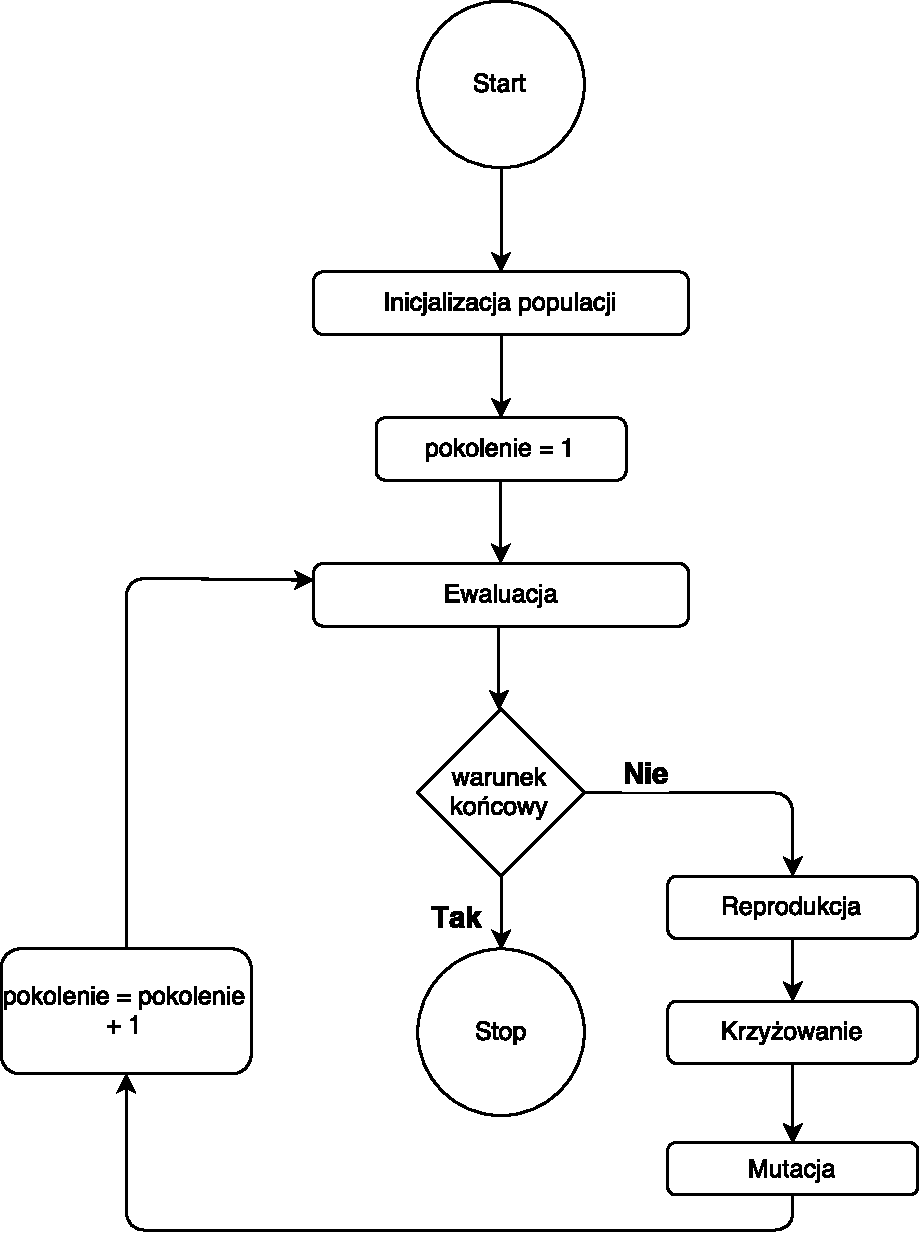
\includegraphics[ clip, scale=0.5]{ga_sequence}}
	\centering
	\caption{Schemat działania algorytmu genetycznego}
	\label{fig:ga_sequence}
\end{figure}

Punktem startowym jest utworzenie losowej populacji osobników. Następnie każdy osobnik jest oceniany przez pryzmat ustalonego kryterium. Na podstawie oceny przeprowadzany jest proces selekcji, czyli wyboru najlepszych osobników, które wykorzystane zostaną do reprodukcji. Podczas procesu reprodukcji generowane są nowe osobniki tworzące kolejne pokolenie. Każdy nowy osobnik jest wynikiem krzyżowania, czyli łączenia chromosomu dwóch rodziców w jeden. Chromosom z punktu widzenia biologii jest formą organizacji materiału genetycznego. Z punktu widzenia algorytmu będzie to zestaw parametrów charakteryzujących danego osobnika, który zostanie opisany później. Następnie chromosomy nowych osobników mogą ulec mutacji, czyli losowej zmianie pojedynczych genów. Gdy zostanie utworzona odpowiednia liczba nowych osobników, czyli powstanie nowe pokolenie, cały proces zaczyna się od początku, dopóki nie osiągnięte zostanie zdefiniowane kryterium końcowe.\\\\
W powyższym opisie pojawiło się kilka pojęć wartych wyjaśnienia.
\subsubsection{Populacja}
Populacja jest grupą o ustalonym rozmiarze. Elementami grupy są pojedyncze osobniki. Jedną z przewag algorytmów genetycznych nad tradycyjnymi technikami optymalizacyjnymi jest właśnie operowanie nie na jednym konkretnym rozwiązaniu, lecz na całej grupie. Duża różnorodność osobników w połączeniu z odpowiednim użyciem operatorów genetycznych pozwala uniknąć problemu ,,utknięcia'' na optimum lokalnym.
\subsubsection{Chromosom}
Chromosom, jak zostało już wspomniane, jest sposobem reprezentacji właściwości cechujących danego osobnika. Chromosom można zdefiniować na dwa sposoby: za pomocą ciągu binarnego lub wartości rzeczywistych. Ciąg binarny jest ciągiem wartości $0$ lub $1$ ułożonych w taki sposób aby odpowiednio zakodować przekazywaną informację. W ramach przykładu załóżmy, że mamy dany cylinder o średnicy $d = 10\text{ }cm$ oraz wysokości $h = 14\text{ }cm$ \cite{book}. Rysunek \eqref{fig:cylinder} pokazuje przykładowy sposób reprezentacji takiego cylindra w formie ciągu binarnego. 
\begin{figure}[!htb]
	\makebox[\textwidth]{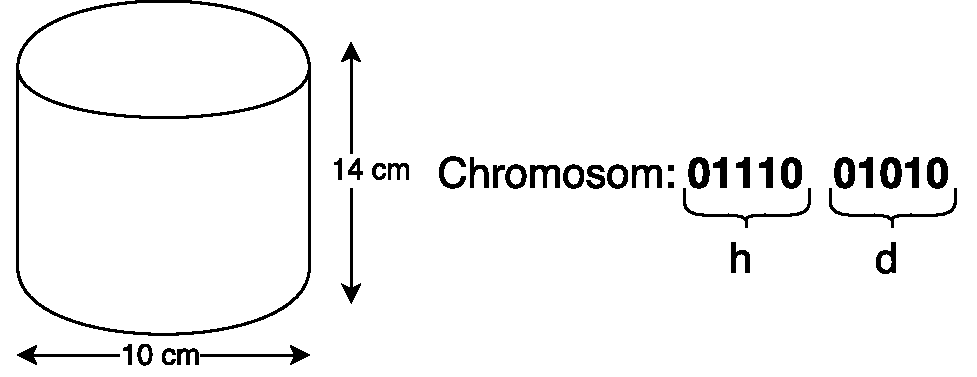
\includegraphics[ clip, scale=0.5]{cylinder}}
	\centering
	\caption{Przykład ciągu binarnego}
	\label{fig:cylinder}
\end{figure}
\\Chromosom reprezentujący cylinder złożony jest z 10 bitów. Na pierwszych pięciu z nich zakodowana jest informacja o wysokości, a na kolejnych informacja o średnicy. Wartości przedstawione przez poszczególne części ciągu należy traktować jak liczby binarne i w ten sam sposób je interpretować.

W większości przypadków preferowane jest używanie ciągu binarnego jako sposobu reprezentacji osobników. Jednym z powodów jest łatwość przeprowadzania operacji krzyżowania oraz mutacji, o których mowa będzie później. Używając reprezentacji binarnej można w prosty sposób zmienić sposób kodowania osobników bez konieczności ingerowania w operatory genetyczne - operatory krzyżowania oraz mutacji nie biorą pod uwagę sposobu w jaki informacja została zapisana w chromosomie. Kolejne argumenty przemawiające za użyciem takiej reprezentacji przedstawione zostały w pracach Goldberga \cite{goldberg} oraz Reeves'a \cite{reeves}. Kolejne etapy działania algorytmów genetycznych wyjaśnione zostaną przy założeniu, że osobniki przedstawione są za pomocą ciągów binarnych.
\subsubsection{Ewaluacja}
Po ustaleniu sposobu reprezentacji osobników należy wygenerować losową populację oraz poddać ją ocenie, czyli ewaluacji. Proces ewaluacji polega na przypisaniu każdemu osobnikowi odpowiedniej wartości pozwalającej ocenić go na tle reszty populacji. Jest to wartość dopasowania osobnika. Korzystając z wcześniejszego przykładu załóżmy, że podczas procesu ewaluacji zdefiniowanemu wcześniej cylindrowi przypisywany jest koszt wyprodukowania, wyrażony następującym wzorem:
\begin{equation}
f(d,h) = c\big{(}\dfrac{\pi d^{2}}{2} + \pi dh\big{)}
\end{equation}
, gdzie $c$ oznacza koszt materiału na $cm^{2}$ \cite{book}.\\
Zgodnie z podanymi wcześniej danymi oraz przy założeniu, ze $c = 0.01$ koszt wyprodukowania danego cylindra wynosi:
\[f(10, 14) = 6\]
Zakładając, że celem procesu optymalizacji jest minimalizacja kosztu wyprodukowania cylindra, należy zauważyć, że osobnik z przypisaną mniejszą wartością jest lepszy w kontekście wybranego kryterium.
\subsubsection{Reprodukcja}
Kolejnym etapem działania algorytmu genetycznego jest reprodukcja inaczej zwana też selekcją. Jest to proces mający na celu zwiększenie liczby dobrych osobników w populacji oraz redukcję liczby tych gorszych, jednocześnie utrzymując niezmieniony rozmiar całej populacji. Jest to osiągane poprzez realizację następujących zadań \cite{book}:\\
\begin{enumerate}
	\item Zidentyfikowanie dobrych (ocenionych powyżej średniej) osobników.
	\item Utworzenie kopii dobrych osobników.
	\item Eliminację osobników gorszych, tak aby kopie dobrych mogły zostać dodane do populacji.\\
\end{enumerate}
Powyższe zadania mogą zostać osiągnięte przy użyciu kilku metod. Najpopularniejszymi z nich są: metoda turniejowa, metoda ruletki oraz metoda rankingu.

Metoda turniejowa polega na rozgrywaniu turniejów pomiędzy kilkoma osobnikami wybranymi losowo z populacji \cite{tournament}. Zwycięzca każdego turnieju, jako rodzic, przechodzi do etapu krzyżowania, który zostanie opisany później \eqref{fig:tournament}. Rozmiar pojedynczego turnieju znacząco wpływa na przebieg procesu selekcji. Im jest większy, tym mniejsza szansa, że słabsze osobniki przejdą do kolejnego etapu. Wbrew pozorom takie zachowanie nie jest pożądane ze względu na potrzebę zachowania różnorodności populacji. Im rozmiar jest większy tym większa szansa, że do kolejnego etapu dostanie się zbyt dużo słabszych osobników, co również nie jest dobrym rozwiązaniem. Jeśli rozmiar turnieju $S = 1$ selekcja staje się równoważna losowemu wyborowi osobnika. Najczęściej stosuje się turnieje o rozmiarze 2. Metoda turniejowa jest jedną z najczęściej wybieranych metod selekcji. Jest prosta w implementacji oraz pozwala na łatwe manipulowanie rozmiarem turnieju, co z kolei wpływa na szybkość zbliżania się znalezionych rozwiązań do rozwiązań optymalnych. Ponadto jak zostało udowodnione selekcja turniejowa zawsze zapewnia lepszą lub taką samą szybkość zbliżania się do rozwiązań optymalnych jak inne metody selekcji oraz mniejszą lub taką samą złożoność obliczeniową \cite{book}. Z wymienionych powyżej powodów to właśnie metoda turniejowa została zaimplementowana w wybranych algorytmach.
\begin{figure}[!htb]
	\makebox[\textwidth]{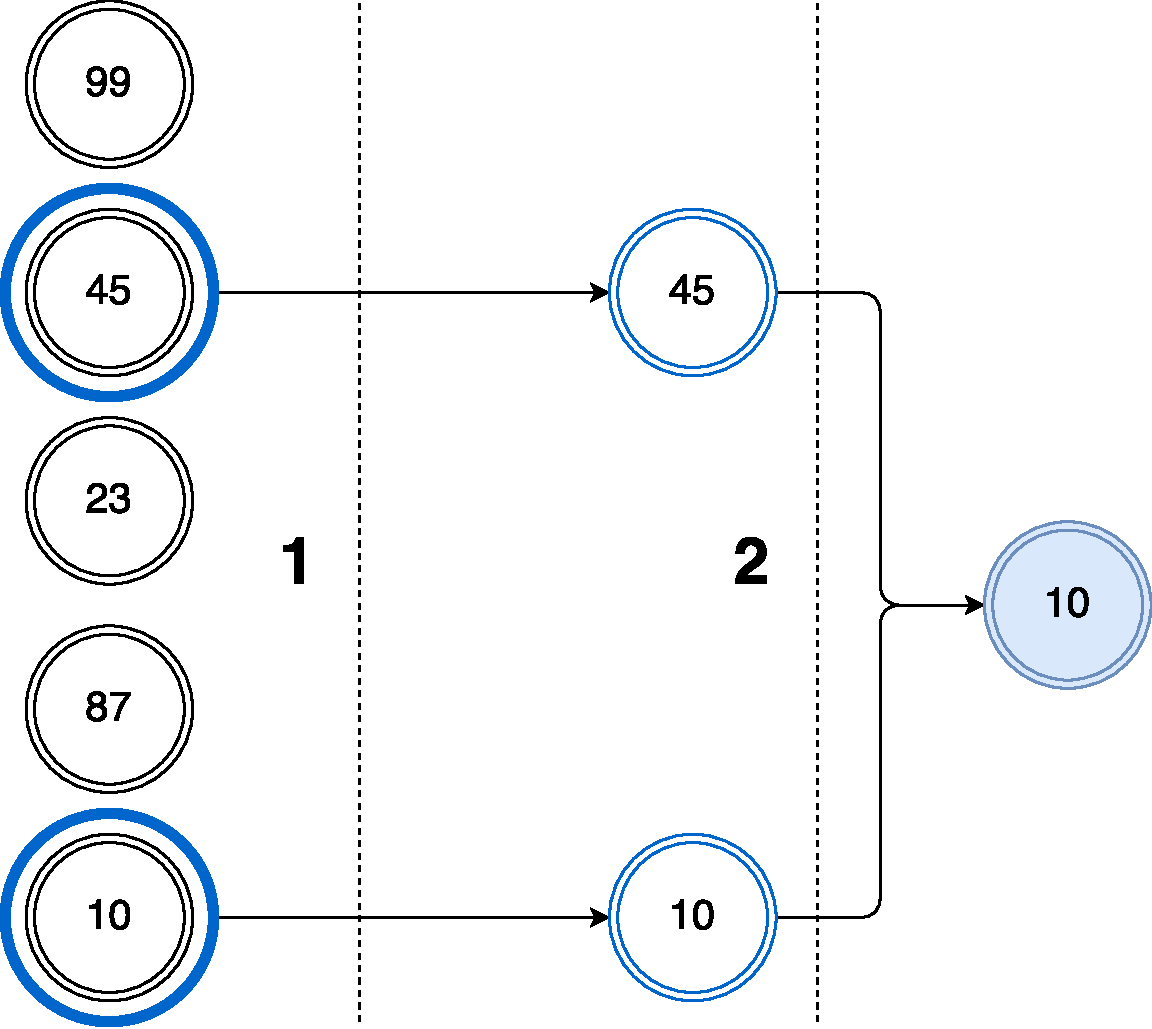
\includegraphics[ clip, scale=0.5]{tournament}}
	\centering
	\caption{Przykład rozegranego turnieju o rozmiarze 2.\\1. Wybór losowych osobników; 2. Turniej pomiędzy wybranymi osobnikami.}
	\label{fig:tournament}
\end{figure}

Kolejną popularną metody selekcji jest metoda proporcjonalna \cite{book}. W metodzie tej wprowadzone zostaje pojęcie puli rozrodczej. Jest to pula spośród której wybierane są osobniki wykorzystywane później do krzyżowania. Wypełnienie puli rozrodczej kopiami osobników wykonywane jest procesie selekcji. Liczba kopii danego osobnika w puli jest proporcjonalna do jego wartości dopasowania. Jeśli średnia wartość dopasowania dla całej populacji wynosi $f_{avg}$, dany osobnik $s_{i}$ będzie posiadał $f_{i}/f_{avg}$ kopii w puli rozrodczej. Metoda proporcjonalna często nazywana jest również metodą ruletki, ponieważ właśnie za pomocą koła ruletki można zobrazować sobie jej działanie. Wspomniane koło jest podzielone na $N$ części, gdzie $N$ jest wielkością populacji. Każdy wycinek koła odpowiada jednemu osobnikowi z populacji. Wielkość danego wycinka jest proporcjonalna do wartości dopasowania osobnika. Wynika z tego, że wycinki powiązane z lepszymi osobnikami będą zajmować większą część koła. Jak można zauważyć na rysunku \eqref{fig:roulette} osobnik o numerze 6 jest najlepszy na tle całej populacji, natomiast osobnik o numerze 2 jest osobnikiem najgorszym. Wybór osobników do puli rozrodczej odbywa się poprzez kręcenie kołem. Czynność ta powtarzana jest $N$ razy. Po zatrzymaniu wybierany jest osobnik na którego wycinku zatrzymał się wskaźnik. Osobniki z najlepszą wartością dopasowania mają największe szanse na trafienie do puli rozrodczej.

Wadami metody proporcjonalnej jest duża złożoność obliczeniowa oraz problemy ze skalowaniem \cite{book}. Załóżmy, że jeden osobnik jest znacząco lepszy od reszty. Wtedy powiązany z nim wycinek będzie zajmował niemal całe koło, a co za tym idzie prawdopodobieństwo wyboru takiego osobnika będzie zbliżone do 1. W konsekwencji pula rozrodcza będzie w większości zapełniona kopiami jednego osobnika, co prowadzi do braku zróżnicowania. Z drugiej strony jeśli wszystkie osobniki mają bardzo zbliżone wartości dopasowania, każdy z nich ma również podobne prawdopodobieństwo wyboru do puli. Prowadzi to do sytuacji, kiedy każdy osobnik ma dokładnie jedną kopię w puli rozrodczej. Taki proces selekcji nie wnosi żadnej wartości i równie dobrze mógłby zostać pominięty. 
\begin{figure}[!htb]
	\makebox[\textwidth]{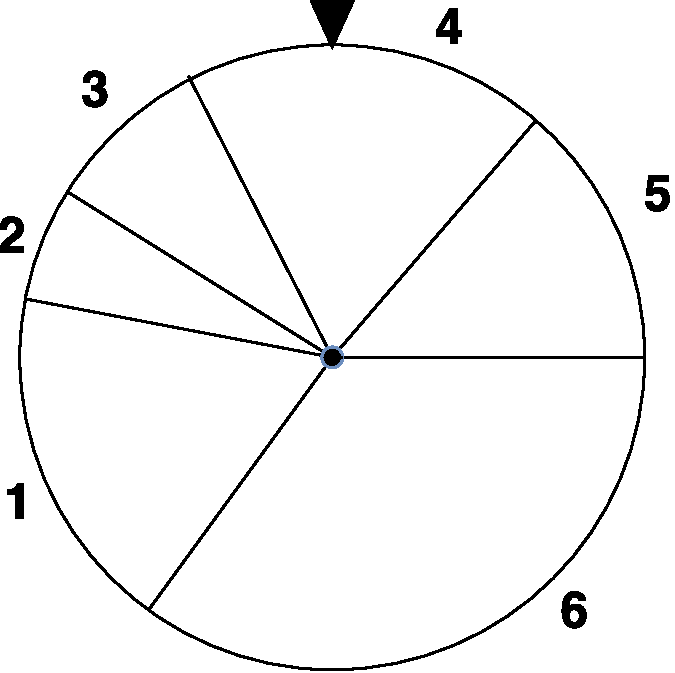
\includegraphics[ clip, scale=0.5]{roulette}}
	\centering
	\caption{Przykładowa wizualizacja selekcji proporcjonalnej}
	\label{fig:roulette}
\end{figure}

Opisanych powyżej problemów ze skalowaniem można uniknąć korzystając z metody rankingowej \cite{book}. Polega ona na posortowaniu osobników z populacji ze względu na ich wartość dopasowania. W ten sposób najgorszemu osobnikowi zostaje przypisane pierwsze miejsce w tworzonym rankingu. Osobnik najlepszy znajdzie się wtedy na $N$-tym miejscu. Po takim przygotowaniu na posortowanej populacji zostaje użyty operator selekcji proporcjonalnej. Na tym etapie przygotowanie koła ruletki nie opiera się już na wartości dopasowania poszczególnych osobników, lecz na ich pozycji w rankingu. Pozwala to na pozbycie się opisanych wcześniej problemów.

\subsubsection{Krzyżowanie}
Po wyborze osobników mających zostać rodzicami następuje czas na skorzystanie z operatora krzyżowania. Tutaj należy zwrócić uwagę na to, że opisany wcześniej proces reprodukcji nie tworzy żadnych nowych osobników. Dzieje się to dopiero w trakcie procesu krzyżowania. Jak wskazuje nazwa, krzyżowanie polega na łączeniu dwóch osobników w celu utworzenia ich potomstwa \cite{ga_book}. Dzieje się to na poziomie zdefiniowanych wcześniej chromosomów. Najprostszą i najlepiej ilustrującą ideę krzyżowania metodą jest metoda jednopunktowa. Polega ona na losowym wybraniu punktu względem którego nastąpi podział chromosomu na dwie części. Potomstwo powstaje na skutek wymiany pomiędzy rodzicami części chromosomu znajdującej się po prawej stronie od wybranego punktu podziału. Proces ten został przedstawiony na rysunku \eqref{fig:one_point_cross}. Po lewej stronie znajdują się chromosomy pary rodziców. Punkt podziału został losowo ustalony na $d=4$, co symbolizuje pionowa przerywana linia. Po prawej stronie znajduje się potomstwo - wynik zastosowania operatora krzyżowania. Jak widać chromosom każdego nowego osobnika powstał na skutek złożenia chromosomów rodziców.
\begin{figure}[!htb]
	\makebox[\textwidth]{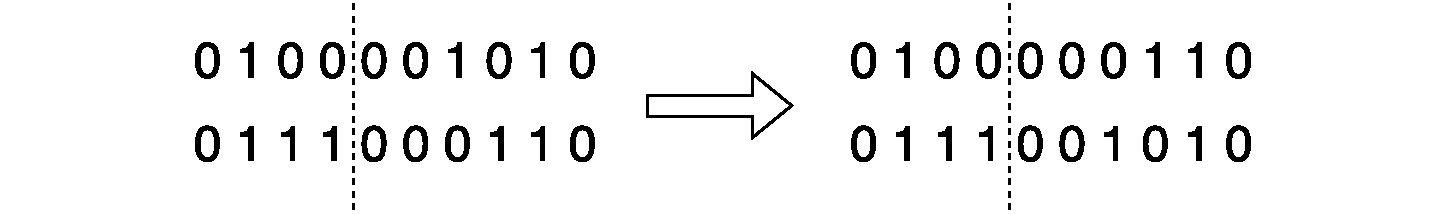
\includegraphics[ clip, scale=0.34]{one_point_cross}}
	\centering
	\caption{Przykład krzyżowania jednopunktowego}
	\label{fig:one_point_cross}
\end{figure}

W tym miejscu należy zauważyć, że nowe osobniki utworzone w procesie krzyżowania niekoniecznie muszą być lepsze od swoich rodziców. Może zdarzyć się tak, że potomstwo będzie gorzej przystosowane. Nie należy się tym jednak martwić, ponieważ jak zostało wyjaśnione wcześniej osobniki o mniejszej wartości przystosowania mają mniejsze szanse na przetrwanie selekcji, a co za tym idzie ich geny nie zostaną przekazane kolejnym pokoleniom. Ponadto jest znacznie bardziej prawdopodobne, że operatory krzyżowania wygenerują rozwiązania lepsze niż generowanie losowe \cite{book}. Dzieje się tak dlatego, że chromosomy wybrane do procesu nie są przypadkowe. Przeszły one selekcje co wskazuje na to, że zawierają w sobie wartościowe kombinacje bitów. Operator krzyżowania użyty na parze rodziców, może wygenerować jedynie $l$ par potomków, gdzie $l$ jest długością chromosomu. Biorąc pod uwagę fakt, że potomstwo jest generowane przy użyciu chromosomów dobrych osobników, istnieje duże prawdopodobieństwo, że utworzone rozwiązania również będą dobre.

Opisany powyżej proces krzyżowania może zostać przeprowadzony również przy użyciu kilku punktów podziału. Na rysunku \eqref{fig:two_point_cross} przedstawiona jest selekcja dwupunktowa. Chromosom dzielony jest na trzy części. Potomstwo powstaje na skutek wymiany części środkowej.
\begin{figure}[!htb]
	\makebox[\textwidth]{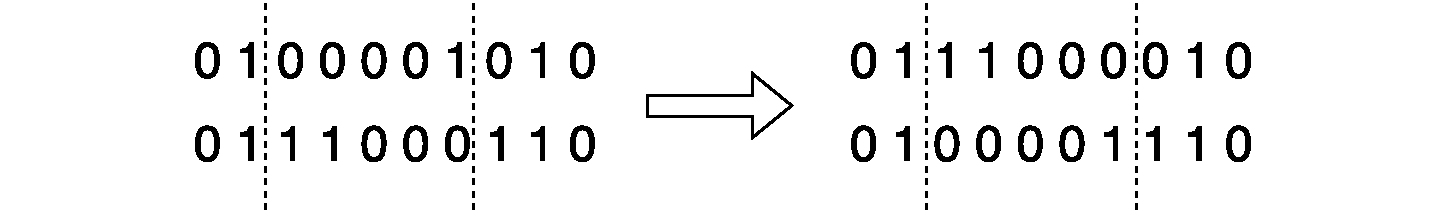
\includegraphics[ clip, scale=0.5]{two_point_cross}}
	\centering
	\caption{Przykład krzyżowania dwupunktowego}
	\label{fig:two_point_cross}
\end{figure}

Przedstawioną ideę podziału chromosomu można dowolnie rozszerzać. Ekstremum jest tzw. podział jednolity \cite{book}. W takim przypadku potomstwo powstaje poprzez wymianę pojedynczych bitów z określonym prawdopodobieństwem $p$. Najczęściej przyjmuje się, że $p = 0.5$, czyli istnieję 50\% szansy, że dany bit zostanie wymieniony na ten pochodzący z drugiego rodzica.

W wybranych algorytmach zastosowano metodę krzyżowania dwupunktowego, która jest typowym wyborem przy chromosomach reprezentowanych za pomocą ciągów binarnych \cite{sensors}.

W celu zachowania części dobrych osobników z populacji, do procesu krzyżowania dodaje się dodatkową zmienną $p_{c}$, oznaczająca prawdopodobieństwo krzyżowania \cite{ga_book}. Oznacza ona jaka część obecnej populacji zostanie użyta do procesu krzyżowania. Gdy $p_{c} = 1$ nowa populacja w całości zostanie zapełniona potomkami osobników ze starej populacji. W innym przypadku $100(1 - p_{c})\%$ osobników ze starej populacji zostanie skopiowanych do nowej. Najczęściej prawdopodobieństwo krzyżowania ustawia się na poziomie 80-90\%.

\subsubsection{Mutacja}
Nowe osobniki powstałe na skutek krzyżowania mogą ulec mutacji. Mutacja jest odpowiedzialna za losową modyfikację chromosomu danego osobnika. Operator mutacji zapewnia utrzymanie różnorodności populacji na odpowiednim poziomie \cite{ga_book}. Działanie tego operatora opiera się na zmiennej wyrażającej prawdopodobieństwo mutacji: $p_{m}$. Operator nie działa na poziomie całego chromosomu, lecz pojedynczych bitów, a jego zastosowanie jest równoznaczne ze zmianą wartości danego bitu. Zostało to zilustrowane na rysunku \eqref{fig:mutation}.
\begin{figure}[!htb]
	\makebox[\textwidth]{
\includegraphics[ clip, scale=0.5]{mutation}}
	\centering
	\caption{Przykład mutacji}
	\label{fig:mutation}
\end{figure}

Podobnie jak w przypadku zastosowania operatora krzyżowania tak i w przypadku mutacji, osobnik będący rezultatem może okazać się gorszy od oryginału. Mimo to, warto zauważyć, że używanie operatora mutacji przy użyciu niskiego prawdopodobieństwa $p_{m}$ nie jest operacją losową \cite{book}. Powodem jest to, że rozwiązanie generowane jest na podstawie już istniejącego osobnika oraz cały proces może utworzyć jedynie kilka nowych rozwiązań, z dużym prawdopodobieństwem, również dobrych.\\

Podsumowując, algorytmy genetyczne używają trzech operatorów: selekcji, krzyżowania oraz mutacji. Operator selekcji odpowiedzialny jest za wybór najlepiej przystosowanych osobników. Operator krzyżowania służy do łączenia wybranych wcześniej osobników w celu utworzenia potomstwa. Operator mutacji losowo zmienia część chromosomu danego osobnika w nadziei na znalezienie jeszcze lepszego rozwiązania. Należy tutaj zwrócić uwagę, że żaden z opisanych operatorów nie jest deterministyczny. Każdy z nich oparty jest w znacznym stopniu o losowość, co powoduje, że nie zawsze będą one osiągać zamierzone rezultaty. Nie mniej jednak w kontekście działania algorytmu wymagane jest, aby gorsze osobniki były eliminowane w procesie reprodukcji, na rzecz osobników lepszych, których geny powinny być przekazywane do kolejnych pokoleń.
\section{Algorytmy wielokryterialne}
Główną różnicą pomiędzy klasycznymi metodami optymalizacji, a algorytmami genetycznymi jest fakt, że te drugie nie operują na jednym rozwiązaniu ale na całej populacji rozwiązań. Różnica ta daje ogromną przewagę algorytmom genetycznym jeśli chodzi o rozwiązywanie wielokryterialnych problemów optymalizacyjnych. Jak zostało wspomniane w rozdziale dotyczącym optymalizacji wielokryterialnej, jej celem jest znalezienie jak największej liczby rozwiązań optymalnych w sensie Pareto. Algorytmy genetyczne dają możliwość znalezienia grupy takich rozwiązań jako rezultatu uruchomienia jednej symulacji \cite{book}. Eliminuje to konieczność wielokrotnego używania metod optymalizacji jednokryterialnej w celu znajdowania kolejnych optymalnych rozwiązań. Ponadto używając algorytmów genetycznych można pozbyć się wielu parametrów koniecznych przy używaniu metod klasycznych. Przykładem może być chociażby wektor wag, wykorzystywany do transformacji problemu wielokryterialnego w problem jednokryterialny. Jest on konieczny, ponieważ konkretne ustawienie takiego wektora jest ściśle powiązane z jednym znalezionym rozwiązaniem optymalnym. Jeśli chcemy znaleźć inne rozwiązanie należy zmienić ustawienia wektora oraz ponownie uruchomić symulację \cite{book}. W przypadku algorytmów genetycznych nie będzie to konieczne, ponieważ jak zostało wspomniane rezultatem zwróconym przez taki algorytm będzie nie pojedyncze rozwiązanie ale cała grupa rozwiązań.

Co więcej operatory genetyczne mogą zostać zmodyfikowane tak, aby faworyzować rozwiązania niezdominowane oraz jednocześnie utrzymywać różnorodność populacji na odpowiednim poziomie. Te dwie cechy połączone z ogólna ideą algorytmów genetycznych prowadzą do znalezienia zróżnicowanej grupy osobników optymalnych w sensie Pareto, czyli rozwiązania wielokryterialnego problemu optymalizacyjnego.

W kolejnych podrozdziałach opisane zostaną dwa algorytmy spełniające powyższe założenia: NSGA-II oraz SPEA. Wyjaśnione zostanie na jakich zasadach działają oba algorytmy oraz w jaki sposób modyfikują poszczególne operatory genetyczne.
\subsection{NSGA-II}
NSGA-II jest drugą wersją zaproponowanego w 2000 roku algorytmu NSGA (Elitist Non-Dominated Sorting Genetic Algorithm). Jego działanie opiera się na dwóch konceptach: elitaryzmie oraz strategii zachowania różnorodności w populacji \cite{nsga}. 

\subsubsection{Elitaryzm}
Elitaryzm jest dodatkowym operatorem używanym w algorytmach genetycznych. Jego rolą jest zwiększenie szansy, że najlepsze rozwiązania z danego pokolenia (elita) zostaną bezpośrednio przeniesione do pokolenia następnego. Istnieje wiele sposobów na zdefiniowanie operatora elitaryzmu. W przypadku problemów jednokryterialnych przykładem może być porównywanie potomków utworzonych w procesie krzyżowania z ich rodzicami oraz zachowanie dwóch najlepszych osobników. Z globalnego punktu widzenia elitaryzm może być wprowadzony poprzez łączenie rodziców oraz potomków w jedną populację, na której używane są później operatory genetyczne. W ten sposób rodzice dostają szanse na rywalizację ze swoim potomstwem.

Celem elitaryzmu jest zapewnienie, że wartość przystosowania najlepszego osobnika w danym pokoleniu nie jest gorsza od jego odpowiednika z poprzedniego pokolenia. Operator elitaryzmu gwarantuje, że najlepsze rozwiązania znalezione na początku symulacji nie zostaną zgubione. Ponadto ich obecność w kolejnych populacjach zwiększa szanse na utworzenie lepszego potomstwa. 

Podsumowując, odpowiednio użyty elitaryzm zapewnia lepsze działanie algorytmów genetycznych. Należy jednak zwrócić uwagę na to jaki procent najlepszych osobników można nazwać elitą. Jest to określane przez zmienną $\alpha$. Jeśli procent ten jest duży, prawdopodobne jest, że w następnych pokoleniach populacja zacznie skupiać się wokół najlepszych osobników, prowadząc do zmniejszenia różnorodności. Jeśli procent będzie za mały wpływ elitaryzmu może zostać nadmiernie zredukowany nie wprowadzając żadnego pozytywnego efektu.\\

W NSGA-II początkowym krokiem jest połączenie populacji rodziców $P_{t}$ z populacją potomstwa $Q_{t}$ \cite{nsga}. Wskutek tego powstaje grupa $R_{t}$ o rozmiarze $2N$, gdzie $N$ jest rozmiarem populacji. Jest to grupa, na której będzie pracował algorytm. Następnym krokiem jest poddanie $R_{t}$ sortowaniu rozwiązań niezdominowanych, które zostało opisane w rozdziale poświęconym optymalizacji wielokryterialnej. Następnie tworzona zostaje nowa populacja $P_{t+1}$ o rozmiarze $N$. Dzieje się to poprzez wypełnianie nowej populacji osobnikami należącymi do danego frontu grupy $R_{t}$, zaczynając od frontu najlepszego, czyli pierwszego. Proces ten jest kontynuowany aż do momentu kiedy w nowej populacji nie ma już miejsca na kolejne osobniki. Warto zwrócić uwagę, że osobniki przenoszone są z grupy o rozmiarze $2N$ do grupy o rozmiarze $N$. Przez to nie wszystkie fronty mogą zostać w całości wykorzystane. Fronty, które nie mieszczą się w nowej populacji są po prostu usuwane. Inaczej wygląda sytuacja, gdy dany front może zmieścić się tylko częściowo. Zostało to przedstawione na rysunku \eqref{fig:nsga2_fronts}. W takiej sytuacji na danym froncie stosowane jest sortowanie oparte o lokalną wartość zagęszczenia, która zdefiniowana zostanie później. Następnie do nowej populacji zostaje przeniesionych $n$ brakujących osobników, które podczas sortowania zostały uznane za najlepsze.
\begin{figure}[!htb]
	\makebox[\textwidth]{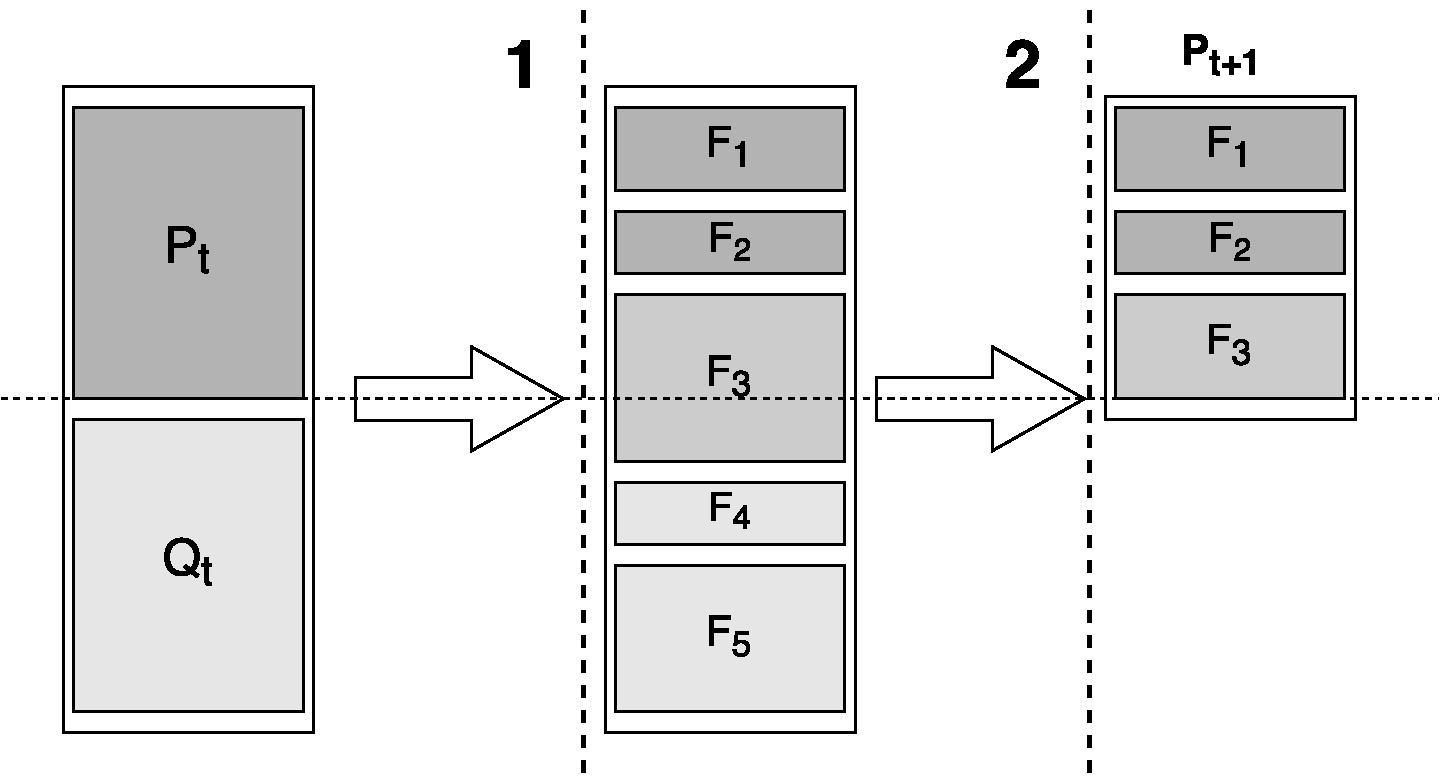
\includegraphics[ clip, scale=0.5]{nsga2_fronts}}
	\centering
	\caption{Uproszczony schemat działania algorytmu NSGA-II.\\1.Sortowanie rozwiązań niezdominowanych.\\2.Sortowanie w oparciu o lokalną wartość zagęszczenia.}
	\label{fig:nsga2_fronts}
\end{figure}

Na nowej populacji $P_{t+1}$ stosowany jest następnie zmodyfikowany operator selekcji \cite{nsga}. Użycie takie operatora zakłada, że każdy osobnik charakteryzuje się dwoma cechami:\\
\begin{enumerate}
	\item Numerem frontu, na którym się znajduje.
	\item Lokalną wartością zagęszczenia.\\
\end{enumerate}
Bazując na tych dwóch cechach, osobnik $i$ jest lepszy od osobnika $j$, jeśli:\\
\begin{enumerate}
	\item Osobnik $i$ znajduje się na lepszym froncie niż osobnik. $j$
	\item Osobnik $i$ znajduje się na tym samym froncie co osobnik $j$ ale charakteryzuje się mniejszą lokalną wartością zagęszczenia.\\
\end{enumerate}
Pierwszy warunek jest odzwierciedleniem koncepcji dominacji. Osobnik leżący na lepszym froncie dominuje osobnika znajdującego się na froncie gorszym. Drugi warunek został wprowadzony, aby rozstrzygać, który z osobników jest bardziej wartościowy jeśli oba leżą na tym samym froncie. Jak zostało wyjaśnione wcześniej rozwiązując wielokryterialne problemy optymalizacyjne należy skupić się nie tylko na jakości rozwiązań ale również na ich różnorodności. Różnorodność danego rozwiązania na tle całości populacji jest definiowana za pomocą metryki określającej zagęszczenie opisanej w \cite{book}. 

Polega ona na obliczeniu średniego dystansu pomiędzy dwoma najbliższymi sąsiadami danego osobnika, znajdującymi się po jego przeciwnych stronach. Zostało to zilustrowane na rysunku \eqref{fig:nsga2_cd}. Takie obliczenia są przeprowadzane $m$ razy dla każdego osobnika, gdzie $m$ jest liczbą zdefiniowanych kryteriów. Następnie wyniki otrzymane dla każdego kryterium są agregowane do jednej wartości $d_{i}$. Generalnie algorytm obliczający zagęszczenie można przedstawić następująco:\\
\begin{enumerate}
	\item Dla każdego osobnika z populacji przypisz $d_{i} = 0$ oraz zdefiniuj $l$ jako liczbę osobników.
	\item Dla każdego kryterium $m$, posortuj populację względem wartości funkcji oceny danego kryterium $f_{m}$, tworząc wektor $I^{m}$
	\item Pierwszemu i ostatniemu osobnikowi z wektora $I^{m}$ przypisz dużą wartość zagęszczenia: $d_{I^{m}_{1}} = d_{I^{m}_{l}} = \infty$. Reszcie osobników przypisz wartość zagęszczenia korzystając ze wzoru:
	\begin{equation}\label{eq:dist_eq}
		d_{I^{m}_{j}} = d_{I^{m}_{j}} + \dfrac{f_{m}^{(I^{m}_{j+1})} - f_{m}^{(I^{m}_{j-1})}}{f^{max}_{m} - f^{min}_{m}}
	\end{equation}
\end{enumerate}
$I_{j}$ oznacza osobnika znajdującego się na $j$-ej pozycji w posortowanym wektorze $I^{m}$. Wynika z tego, że $I_{1}$ oraz $I_{l}$ są osobnikami charakteryzującymi się kolejno najgorszą oraz najlepszą wartością funkcji oceny w porównaniu do całości populacji. Prawa strona równania \eqref{eq:dist_eq} jest różnicą wartości funkcji oceny dwóch najbliższych sąsiadów osobnika $I_{j}$. Jak łatwo zauważyć różnica ta jest połową obwodu prostokąta przedstawionego na rysunku \eqref{fig:nsga2_cd}. Dodatkowo wyliczony dystans jest dzielony przez różnicę pomiędzy największą ($f^{max}_{m}$), a najmniejszą ($f^{min}_{m}$) wartością przyjmowaną przez funkcję oceny $f_{m}$. 
\begin{figure}[!htb]
	\makebox[\textwidth]{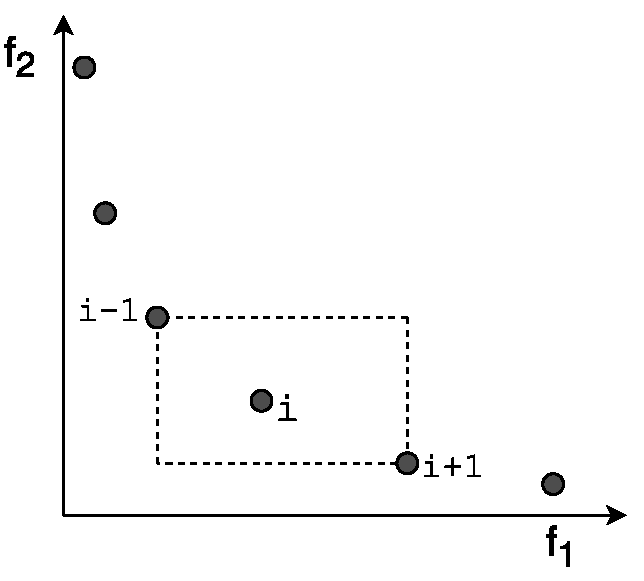
\includegraphics[ clip, scale=0.5]{nsga_2_cd}}
	\centering
	\caption{Reprezentacja najbliższego sąsiedztwa punktu $i$}
	\label{fig:nsga2_cd}
\end{figure}
\\Podsumowując schemat działania algorytmu NSGA-II wygląda następująco:\\
\begin{enumerate}
	\item Połącz populację rodziców $P_{t}$ z populacją potomków $Q_{t}$ tworząc grupę $R_{t}$.
	\item Na $R_{t}$ zastosuj sortowanie rozwiązań niezdominowanych w celu zdefiniowania frontów rozwiązań.
	\item Utwórz nową populację $P_{t+1}$ za pomocą opisanej wcześniej procedury.
	\item Utwórz nową populację potomków $Q_{t+1}$ za pomocą zmodyfikowanego operatora selekcji oraz standardowych operatorów krzyżowania oraz mutacji.\\
\end{enumerate}

W opisanym powyżej algorytmie NSGA-II różnorodność znalezionych rozwiązań niezdominowanych jest zapewniona poprzez zastosowanie zmodyfikowanego operatora selekcji. Osobniki rywalizują ze sobą opierając swoją wartość o front, na którym się znajdują oraz lokalną wartość zagęszczenia. Wartość zagęszczenie staje się szczególnie ważna w późniejszych momentach symulacji, kiedy większość osobników znajduje się już na najlepszym froncie. Biorąc pod uwagę fakt, że algorytm operuje na grupie o rozmiarze $2N$ istnieje duża szansa, że liczba osobników z pierwszego frontu jest większa niż $N$, a więc w celu wybrania najlepszych osobników wzięta zostanie pod uwagę wartość zagęszczenia. W konsekwencji rezultatem będzie zbiór rozwiązań niezdominowanych, cechujący się wysokim stopniem różnorodności \cite{nsga}.
\subsection{SPEA}
SPEA (Strength Pareto Evolutionary Algorithm) jest algorytmem zaproponowanym w 1998 roku \cite{spea}. Koncept elitaryzmu jest tutaj wprowadzony w postaci zewnętrznej populacji $\overline{P}$. W populacji tej przechowywane są wszystkie niezdominowane rozwiązania znalezione w trakcie działania algorytmu. SPEA oprócz przechowywania najlepszych rozwiązań wykorzystuje je także w procesie reprodukcji, co ma znaczący wpływ na jakość generowanych potomków.

Pierwszym krokiem algorytmu jest utworzenie losowej populacji $P_{0}$ oraz pustej zewnętrznej populacji $\overline{P_{0}}$ o ustalonym rozmiarze, nie większym niż $N$, gdzie $N$ jest wielkością populacji $P_{0}$. Na początku każdej iteracji $t$, na populacji $P_{t}$ stosowane jest sortowanie rozwiązań niezdominowanych, w celu znalezienia najlepszego frontu. Osobniki znajdujące się na tym froncie są dodawane do populacji zewnętrznej. Następnie z populacji zewnętrznej usuwane są osobniki zdominowane przez nowo dodane rozwiązania. W ten sposób w populacji zewnętrznej zawsze będą znajdować się jedynie osobniki najlepsze. Łatwo uświadomić sobie, że wraz z działaniem algorytmu wielkość zewnętrznej populacji będzie rosnąć, aż do osiągnięcia zdefiniowanego wcześniej rozmiaru. Gdy ten zostanie osiągnięty pojawia się problem co robić z elitami znajdowanymi w kolejnych pokoleniach, skoro w populacji zewnętrznej nie ma już dla nich miejsca. Rozwiązaniem jest posłużenie jest wartością zagęszczenia, opisaną w poprzednim podrozdziale. Do populacji zewnętrznej trafiają osobniki charakteryzujące się największą różnorodnością na tle populacji. Jak zostało zasugerowane w \cite{book} wartość zagęszczenia może zostać zdefiniowana przy użyciu metryki wykorzystywanej w algorytmie NSGA-II.

Kiedy populacja zewnętrzna zostanie zaktualizowana, następuje proces ewaluacji. Proces ten zostaje najpierw wykonany na populacji zewnętrznej. Dla każdego osobnika $i$ przypisywana zostaje wartość, zdefiniowana jako \textit{siła} $S_{i}$. Siła danego osobnika z zewnętrznej populacji wyrażona jest wzorem:
\begin{equation}\label{eq:str_ep}
	S_{i} = \dfrac{n_{i}}{N + 1}
\end{equation}
, gdzie $n_{i}$ określa liczbę osobników populacji, która jest zdominowana przez osobnika $i$. Jak łatwo zauważyć, osobnik dominujący więcej rozwiązań będzie charakteryzował się większą wartością funkcji $S_{i}$.\\\\
Osobniki z populacji $P_{i}$ ocenianie są przy użyciu następującej funkcji:
\begin{equation}\label{eq:str_p}
	F_{j} = 1 + \sum_{i \in \overline{P_{t}} \wedge i \preceq j} S_{i}
\end{equation}
Liczba $1$ zostaje dodana po to, aby zapewnić, że wartość oceny każdego rozwiązania będzie większa od siły osobników znajdujących się w populacji zewnętrznej. Ponadto dodawana jest suma siły każdego osobnika, przez którego danego rozwiązanie $j$ jest zdominowane. W tym miejscu warto zauważyć, że im mniejsza jest wartość funkcji oceny $F_{j}$, tym lepszy jest dany osobnik. Przykład procesu ewaluacji został przedstawiony na rysunku \eqref{fig:spea_eval}. Osobniki zaznaczone na czerwone należą do populacji zewnętrznej. Jak łatwo zauważyć w procesie reprodukcji faworyzowane będą osobniki charakteryzujące się mniejszą wartością funkcji oceny, a więc te z populacji zewnętrznej.
\begin{figure}[!htb]
	\makebox[\textwidth]{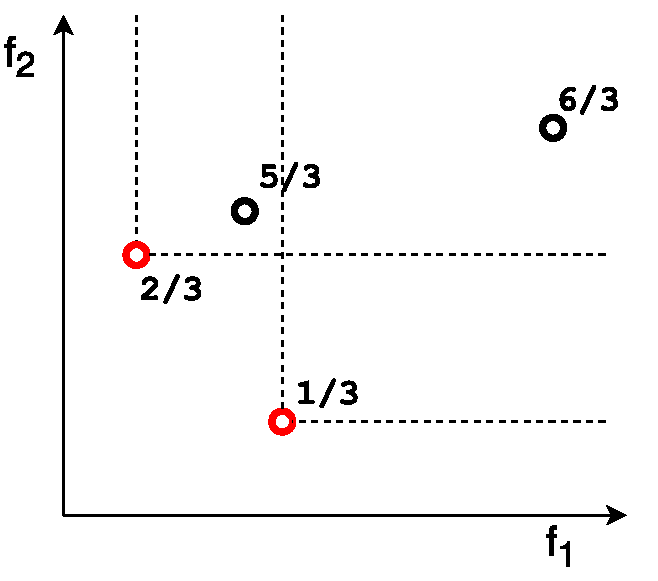
\includegraphics[ clip, scale=0.7]{spea_eval}}
	\centering
	\caption{Przypisanie wartości funkcji oceny}
	\label{fig:spea_eval}
\end{figure}

Po zakończeniu procesu ewaluacji, reszta procesu przebiega według standardowego schematu. Należy jednak pamiętać, że wszystkie operatory genetyczne działają zarówno na populacji $P_{t}$ jak i populacji zewnętrznej $\overline{P_{t}}$.\\\\
Podsumowując schemat działania algorytmu SPEA wygląda następująco:\\
\begin{enumerate}
	\item Zastosuj sortowanie niezdominowanych rozwiązań na populacji $P_{t}$ w celu znalezienia rozwiązań niezdominowanych.
	\item Skopiuj znalezione rozwiązania do populacji zewnętrznej $\overline{P_{t}}$.
	\item Z populacji zewnętrznej usuń rozwiązania zdominowane.
	\item Jeśli rozmiar populacji zewnętrznej jest większy niż $\overline{N}$, zastosuj sortowanie w oparciu o wartość zagęszczenia oraz zredukuj rozmiar populacji zewnętrznej do ustalonej wartości $\overline{N}$ pozbywając się najgorszych osobników.
	\item Oceń wszystkie rozwiązania korzystając z opisanych wzorów \eqref{eq:str_ep}, \eqref{eq:str_p}.
	\item Utwórz nową populacje korzystając z operatorów selekcji, krzyżowania oraz mutacji.\\
\end{enumerate}

Analizując przedstawiony algorytm, łatwo zauważyć, że raz znalezione rozwiązanie optymalne w sensie Pareto nigdy nie przepadnie, ponieważ będzie przechowywane w populacji zewnętrznej. Jedynym sposobem na pozbycie się takiego rozwiązania jest znalezienie kolejnego rozwiązania optymalnego w sensie Pareto, lecz charakteryzującego się lepszą wartością zagęszczenia. Takie podejście zapewnia jakość oraz różnorodność znajdowanych osobników.

Duże znaczenie dla działania algorytmu ma wielkość zewnętrznej populacji $\overline{N}$. Jeśli ta jest duża (porównywalna do $N$)  nacisk na selekcję rozwiązań z populacji zewnętrznej będzie większy, co może prowadzić do tego, że algorytm nie będzie potrafił wygenerować rozwiązań leżących na prawdziwym froncie Pareto. Gdy $\overline{N}$ będzie zbyt małe, wpływ elitaryzmu będzie niezauważalny. Ponadto może to prowadzić do sytuacji w której wiele rozwiązań z populacji nie będzie zdominowanych przez żadnego osobnika z populacji zewnętrznej. Będzie skutkować to tym, że wartość funkcji oceny dla tych osobników będzie tak sama. Proponowaną wielkością populacji zewnętrznej jest $1/4$ wielkości populacji $N$ \cite{book}.

\section{Implementacja}
W obu wybranych algorytmach (NSGA-II, SPEA) pojedynczy osobnik reprezentowany jest jako zbiór zraszaczy $S$. Maksymalna ilość zraszaczy została ustalona na poziomie $ms = 50$. Pojedynczy zraszacz jest reprezentowany jako następujący ciąg bitów:
\begin{figure}[!htb]
	\makebox[\textwidth]{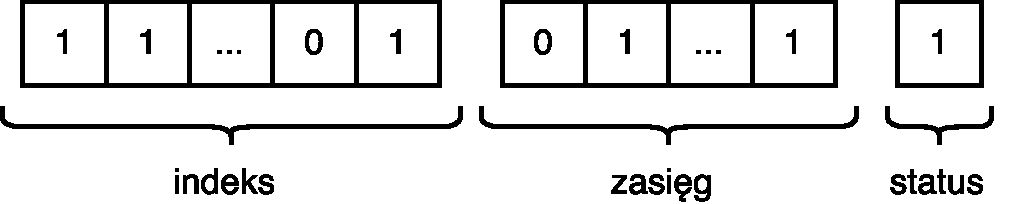
\includegraphics[ clip, scale=0.5]{sprinkler_bin_repr}}
	\centering
	\caption{Reprezentacja bitowa pojedynczego zraszacza}
	\label{fig:sprinkler_bin_repr}
\end{figure}
\\Ciąg binarny podzielony jest na trzy części. Pierwsza z nich odpowiada za indeks, czyli pozycję danego zraszacza. Zraszacz może znajdować się w jednym z kwadratów macierzy $M$, którego środek znajduje się w środku wielokąta $P$. Indeks danego kwadratu jest ustalany według wzoru:
\begin{equation}
	ind_{i} = n_{i} m + m_{i}
\end{equation}
, gdzie $n_{i}$ oznacza wierz macierzy $M$, w którym znajduję się kwadrat $i$; $m$ jest wartością wyrażającą szerokość macierzy; $m_{i}$ oznacza kolumnę macierzy $M$.\\\\
Długość części reprezentującej położenie danego zraszacza wynosi:
\DeclarePairedDelimiter{\ceil}{\lceil}{\rceil}
\begin{equation}
	L_{p} = \ceil[\big]{\log_{2} \text{ } ind_{p}} + 1
\end{equation}
, gdzie $ind_p$ jest liczbą reprezentującą największy indeks należący do $P$.

Kolejną częścią reprezentacji binarnej jest część odpowiadająca za zasięg danego zraszacza. Wymaga ona zużycia $L_{r}$ bitów, gdzie $L_{r}$ jest definiowane jako:
\begin{equation}
	L_{r} = \ceil[\big]{\log_{2} \text{ } r_{max}} + 1
\end{equation}
Wartość $r_{max}$ jest wartością oznaczającą maksymalny zasięg zraszacza. Jest ona definiowana na podstawie zbudowanej bazy danych i określana poprzez wybranie największej wartości zasięgu spośród wszystkich dostępnych.

Ostatnia, trzecia część reprezentacji binarnej to jeden bit mówiący o statusie danego zraszacza. $b = 1$ oznacza, że dany zraszacza został wybrany do rozwiązania oraz będzie uwzględniany w obliczeniach. W przeciwnym wypadku $b = 0$.\\\\
Podsumowując długość chromosomu każdego osobnika z populacji wynosi:
\begin{equation}
	L = ms(L_{p} + L_{r} + 1)
\end{equation}
W tym miejscu warto zauważyć, że długość chromosomu jest zawsze stała. Nieaktywne zraszacze ($b=0$) nie są w żaden sposób usuwane z reprezentacji. Takie podejście niweluje problemy pojawiające się przy użyciu reprezentacji chromosomów o zmiennej długości. Problemy te są najczęściej powiązane z trudnościami w implementacji operatorów krzyżowania oraz selekcji.
\chapter{Rozwiązanie problemu}
\section{System wspomagania decyzji}
System wspomagania decyzji został zaimplementowany w formie aplikacji webowej. Została ona wykonana przy użyciu następujących technologii:\\
\begin{itemize}
	\item Python (PyPy) \cite{pypy}.
	\item Framework Django \cite{django}.
	\item HTML 5.
	\item JavaScript.
	\item CSS.\\
\end{itemize} 
Użytkownik systemu poprzez interfejs graficzny wprowadza dane oraz wybiera opcje, która później przesyłane są na serwer. Na serwerze dane są przekształcane do formatu zrozumiałego przez zaimplementowane algorytmy genetyczne. Po zakończeniu obliczeń rezultaty zwracane są użytkownikowi w czytelnej oraz przejrzystej formie.

W następnej części podrozdziału przedstawiony zostanie przykładowy scenariusz interakcji użytkownika z system, obrazujący jego działanie.

\subsubsection{Interakcja z użytkownikiem}
Po uruchomieniu aplikacji użytkownikowi ukazuje się ekran przedstawiony na rysunku \eqref{fig:gui_1}. Ekran dzieli się na cztery zasadnicze części. Zostały one oznaczone na rysunku odpowiadającymi im liczbami. Część pierwsza jest częścią główną aplikacji. To właśnie do tego obszaru ładowany jest plan ogrodu, na którym użytkownik definiuje teren mający zostać nawodniony oraz określa miejsce źródła wody. To również na tym ekranie prezentowany są wszystkie rezultaty. Część druga jest częścią informacyjną. Tutaj wyświetlane są instrukcje podpowiadające użytkownikowi co w danym momencie powinien zrobić. Trzecia część jest kontenerem na przyciski, za pomocą których użytkownik zatwierdza swoje wybory, anuluje je lub przechodzi do kolejnych etapów. Część czwarta jest przeznaczona na dodatkowe opcje mające wpływ na działanie algorytmów znajdujących się po stronie serwera.
\begin{figure}[!htb]
	\makebox[\textwidth]{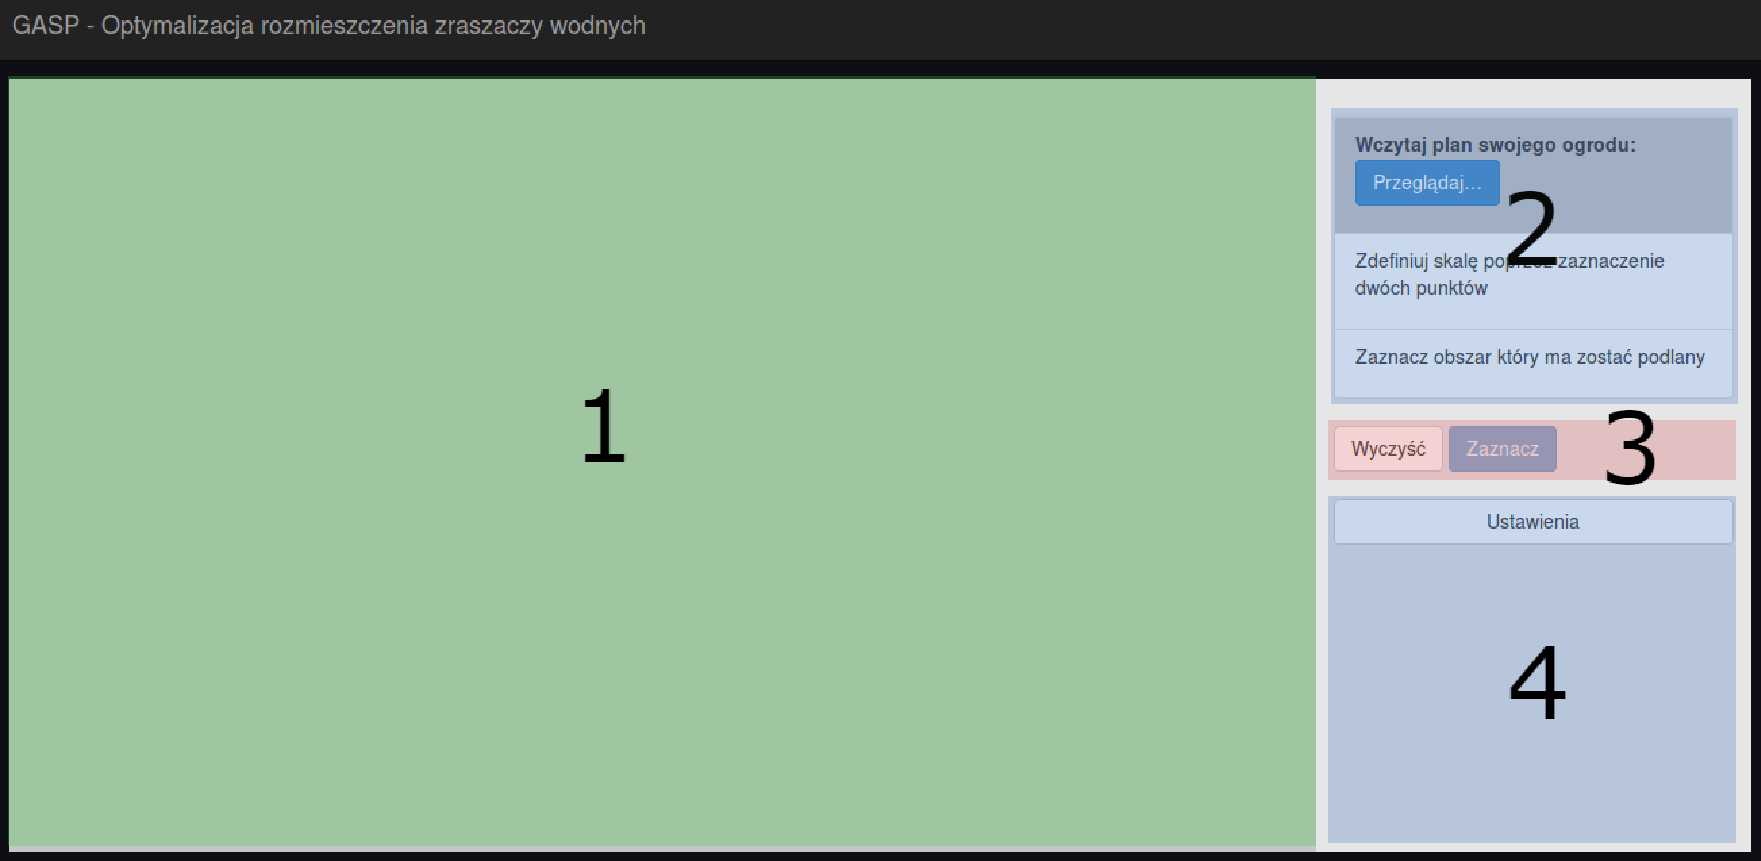
\includegraphics[ clip, scale=0.35]{gui_1}}
	\centering
	\caption{Ekran startowy aplikacji}
	\label{fig:gui_1}
\end{figure}

Pierwszym krokiem w pracy z aplikacją jest wczytanie planu ogrodu. Przykładowy wczytany plan został przedstawiony na rysunku \eqref{fig:gui_2}. Jak można zauważyć zmienił się status panelu informacyjnego widocznego po prawej stronie.
\begin{figure}[!htb]
	\makebox[\textwidth]{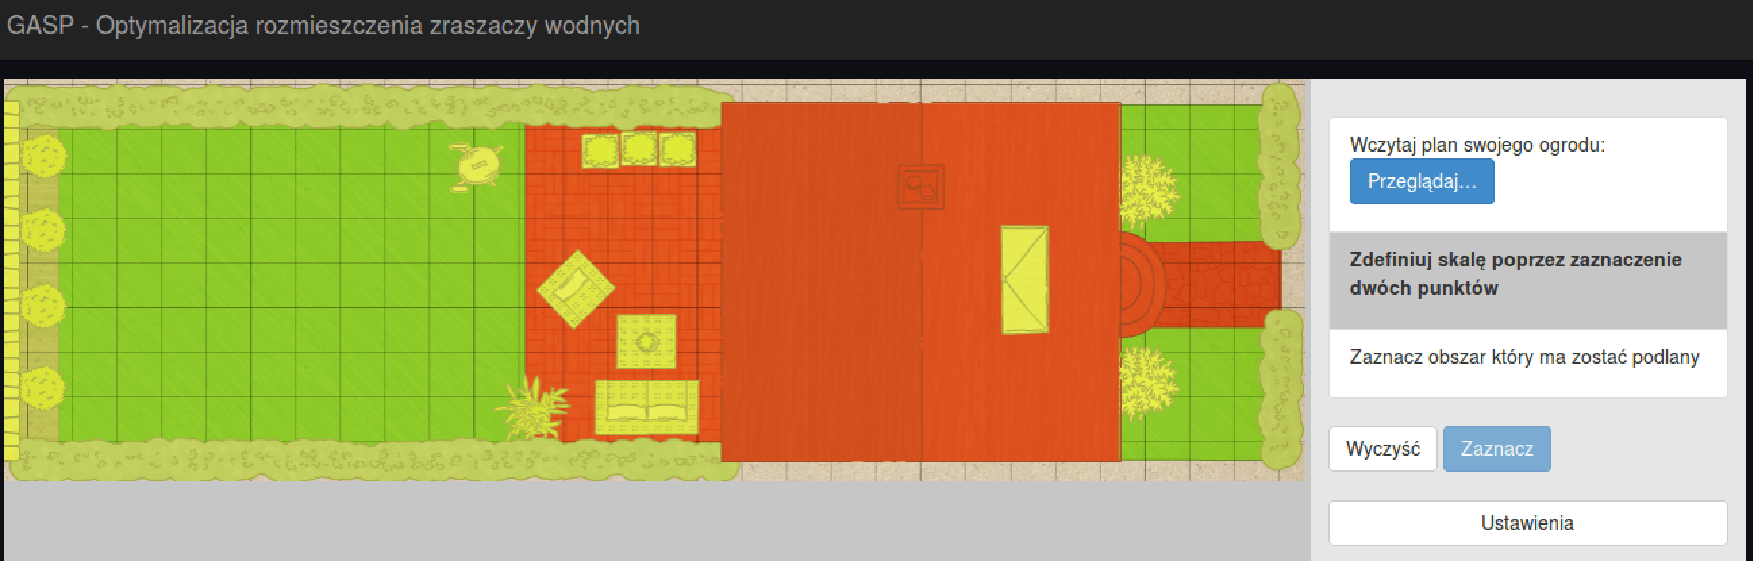
\includegraphics[ clip, scale=0.55]{gui_2}}
	\centering
	\caption{Wczytanie planu ogrodu}
	\label{fig:gui_2}
\end{figure}

Mając wczytany plan ogrodu należy zdefiniować skalę rysunku. Jest to wykonywane poprzez zaznaczenie na wczytanym planie dwóch punktów. Po wykonaniu tej czynności na ekranie pojawia się okno, w którym można zdefiniować dystans pomiędzy zaznaczonymi punktami \eqref{fig:gui_3}.
\begin{figure}[!htb]
	\makebox[\textwidth]{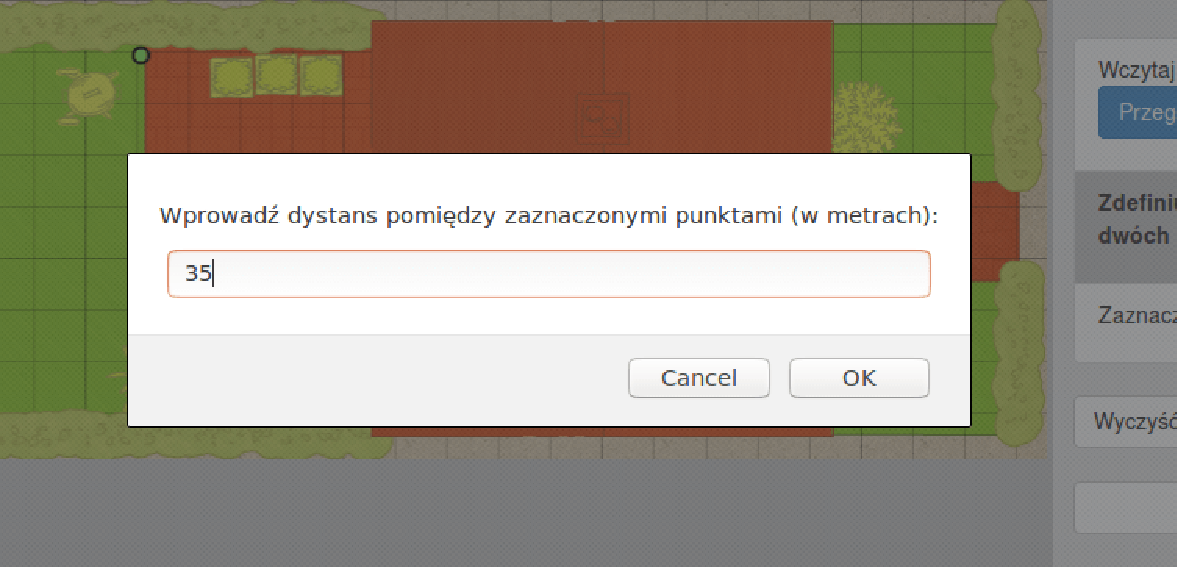
\includegraphics[ clip, scale=0.75]{gui_3}}
	\centering
	\caption{Definiowanie skali wczytanego planu ogrodu}
	\label{fig:gui_3}
\end{figure}

Następnym krokiem jest zaznaczenie na załadowanym planie obszaru, który ma zostać nawodniony. Dzieje się to poprzez określenie, za pomocą lewego przycisku myszy, wierzchołków wielokąta mającego tworzyć wspomniany obszar \eqref{fig:gui_4}. Liczba wierzchołków jest nieograniczona. Po wybraniu obszaru należy rozwinąć panel "Ustawienia". Jak widać w obecnej wersji aplikacji użytkownik może jedynie zdecydować się na to czy chce ograniczyć nawadnianie obszaru poza zaznaczonymi granicami. Aby przejść dalej należy wcisnąć przycisk "Dalej". Spowoduje to przesłanie obecnych ustawień do serwera oraz uruchomienie obliczeń.
\begin{figure}[!htb]
	\makebox[\textwidth]{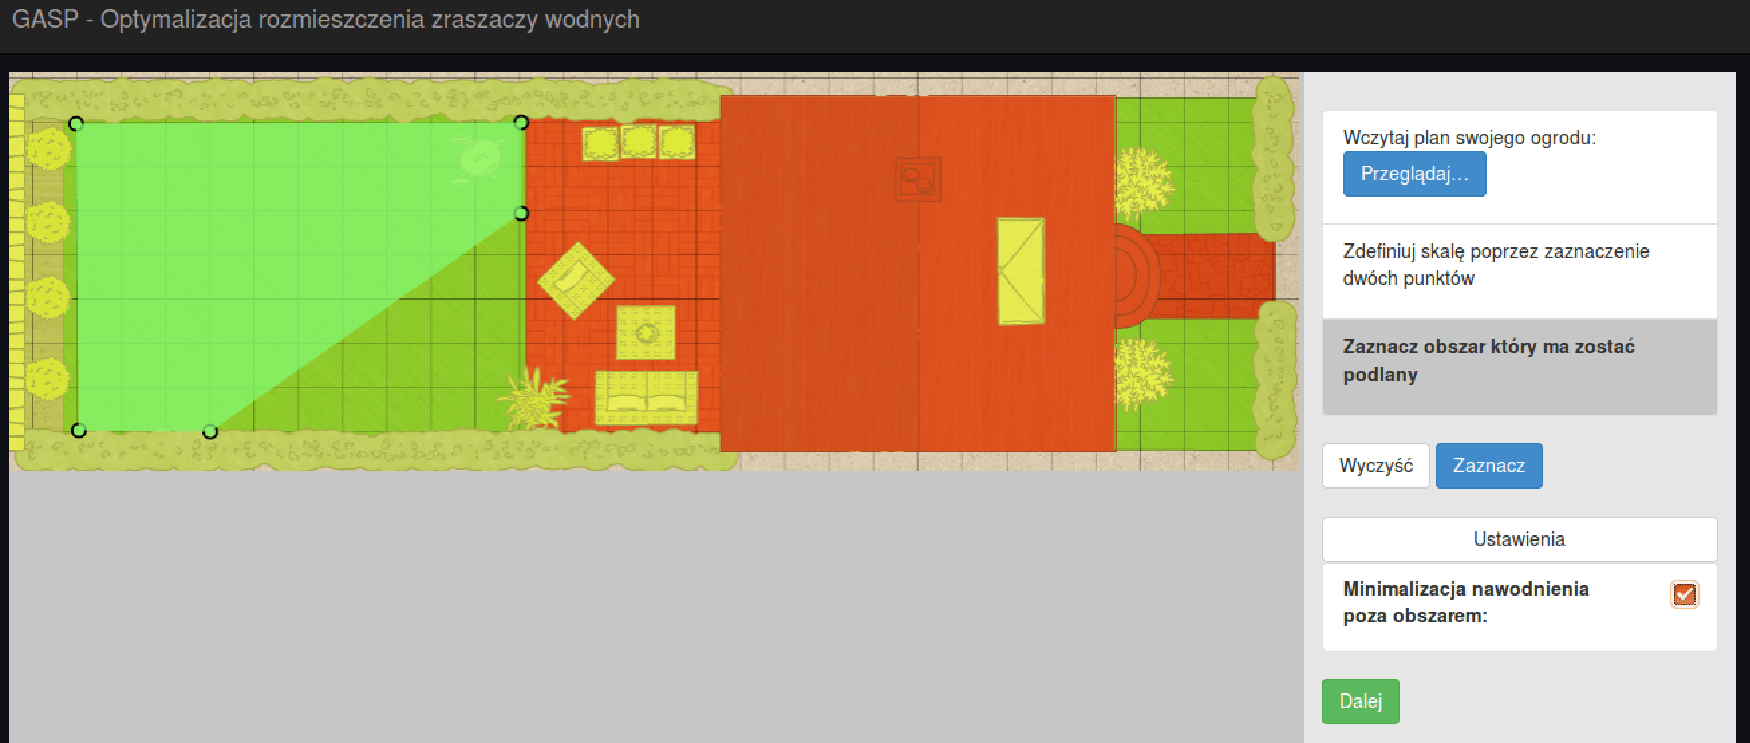
\includegraphics[ clip, scale=0.5]{gui_4}}
	\centering
	\caption{Zaznaczenie obszaru mającego zostać nawodniony}
	\label{fig:gui_4}
\end{figure}

Po zakończeniu działania algorytmu użytkownik zostanie automatycznie przeniesiony na stronę prezentującą listę wyników \eqref{fig:gui_5}. Użytkownik może tutaj wybrać rozwiązanie, które go interesuje oraz podejrzeć je wciskając przycisk ''Zobacz''.
\begin{figure}[!htb]
	\makebox[\textwidth]{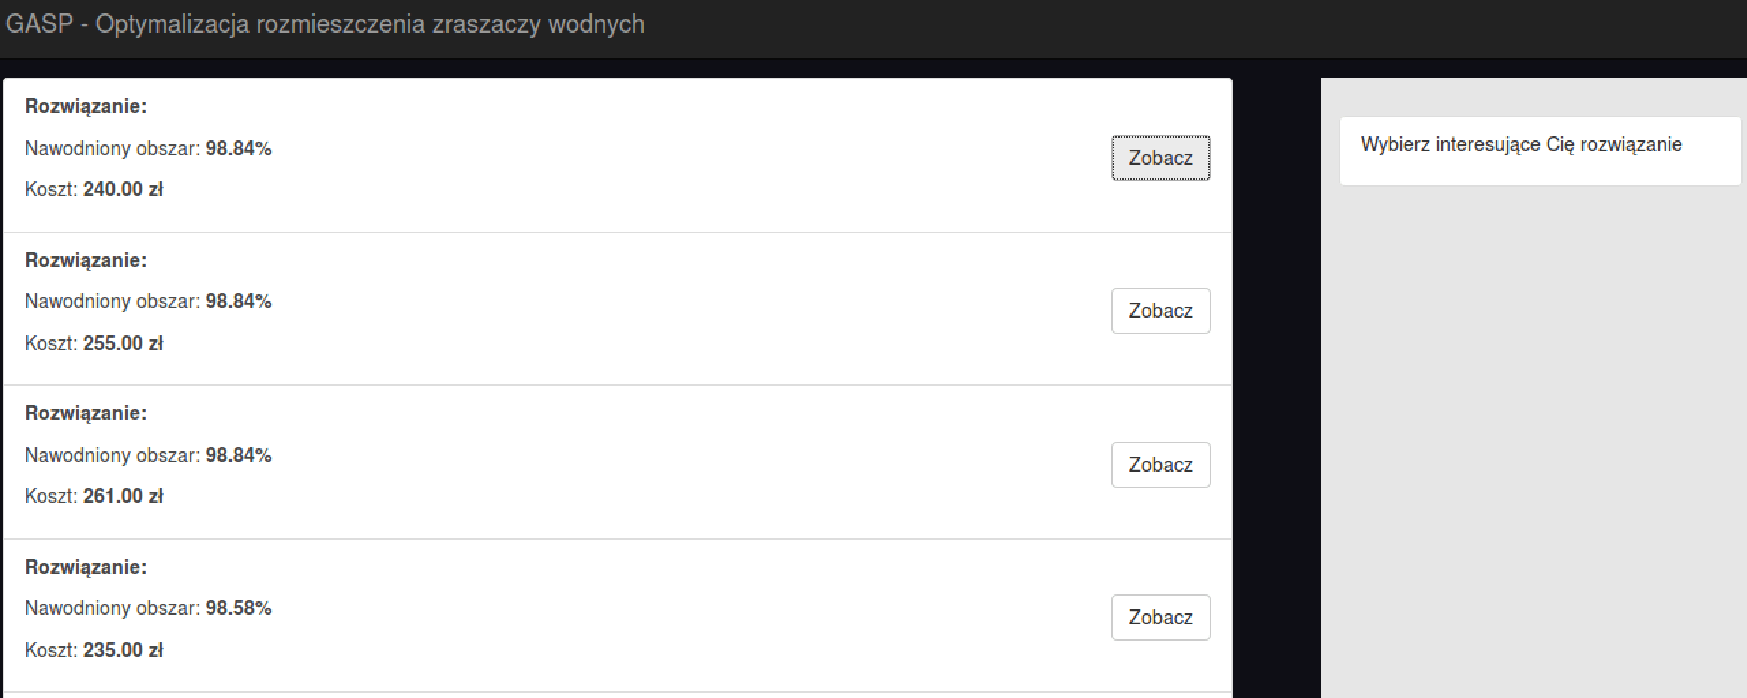
\includegraphics[ clip, scale=0.5]{gui_5}}
	\centering
	\caption{Lista rezultatów}
	\label{fig:gui_5}
\end{figure}

Po wybraniu konkretnego rozwiązania użytkownik zostanie przeniesiony na stronę prezentującą rozmieszczone zraszacze \eqref{fig:gui_6}. Są one zaprezentowane w postaci przezroczystych niebieskich okręgów. Po najechaniu na każdy z nich pojawia się informacja o modelu konkretnego zraszacza, zasięgu oraz cenie. Na tym samym widoku użytkownik może określić, w którym miejscu na planie znajduje się źródło wody. Po wciśnięciu przycisku ''Zakończ'' na planie ogrodu dodatkowo pojawi się schemat poprowadzenia rur \eqref{fig:gui_7}
\begin{figure}[!htb]
	\makebox[\textwidth]{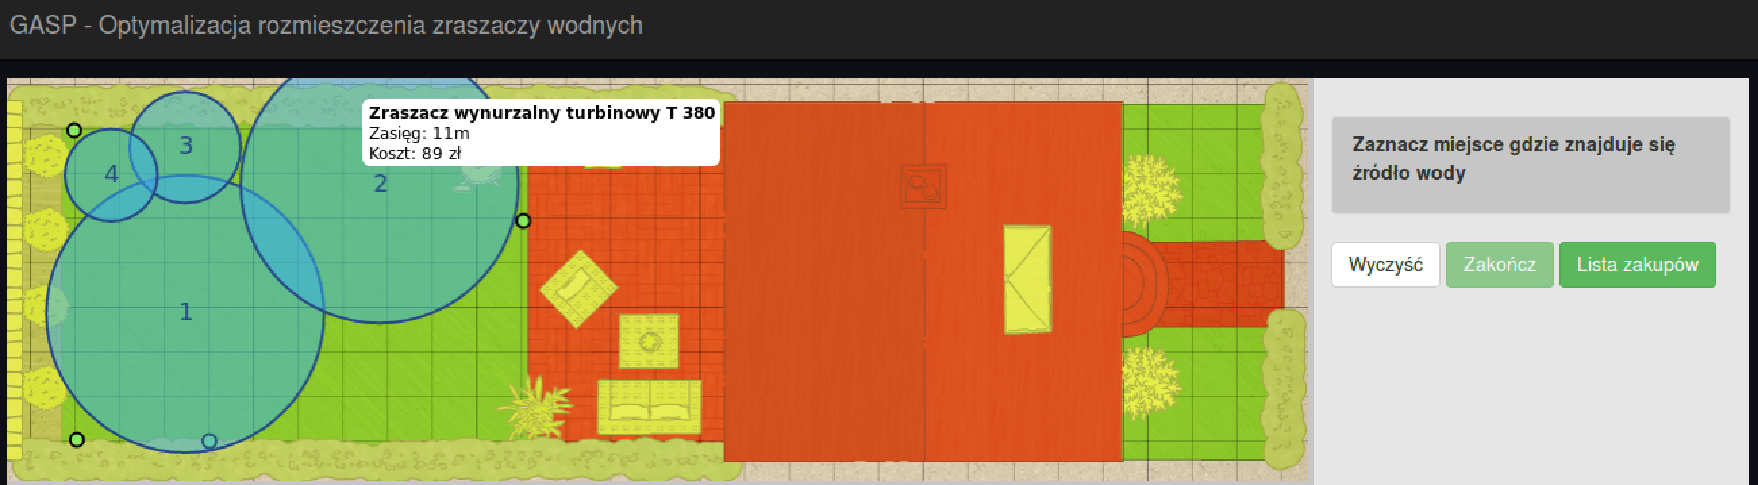
\includegraphics[ clip, scale=0.55]{gui_6}}
	\centering
	\caption{Rozmieszczenie zraszaczy}
	\label{fig:gui_6}
\end{figure}
\begin{figure}[!htb]
	\makebox[\textwidth]{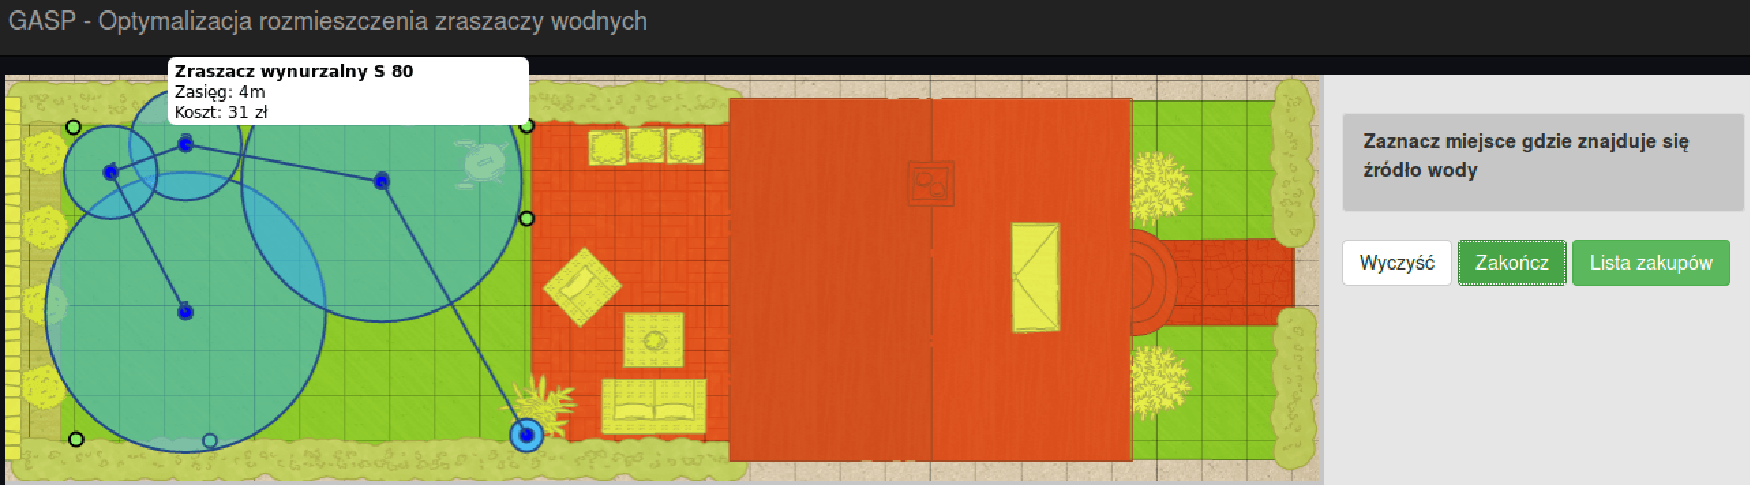
\includegraphics[ clip, scale=0.55]{gui_7}}
	\centering
	\caption{Schemat poprowadzenia rur}
	\label{fig:gui_7}
\end{figure}

W tym momencie użytkownik ma możliwość przejścia do widoku ''Lista zakupów'' \eqref{fig:gui_8}. W tym miejscu warto zauważyć, że lista, znajdująca się po prawej stronie ekranu i pełniąca do tej pory rolę informacyjną, zmieniła się w panel nawigacyjny. Za jej pomocą użytkownik może w łatwy sposób przemieszać się pomiędzy widokami, będącymi podsumowaniem wybranego rozwiązania. Użytkownik ma do wyboru trzy widoki:\\
\begin{enumerate}
	\item Widok rozmieszczonych zraszaczy.
	\item Widok rozmieszczonych zraszaczy oraz schematu poprowadzenia rur.
	\item Widok listy zakupów.\\
\end{enumerate}

Wybierając widok listy zakupów użytkownik zobaczy listę rozmieszczonych zraszaczy. Nazwa każdego zraszacza jest jednocześnie odnośnikiem do opisu konkretnego modelu znajdującego się na stronie producenta. Oprócz tego do każdej pozycji na liście przypisana jest cena. Pod listą znajduje się kwota będąca sumą całych zakupów.
\begin{figure}[!htb]
	\makebox[\textwidth]{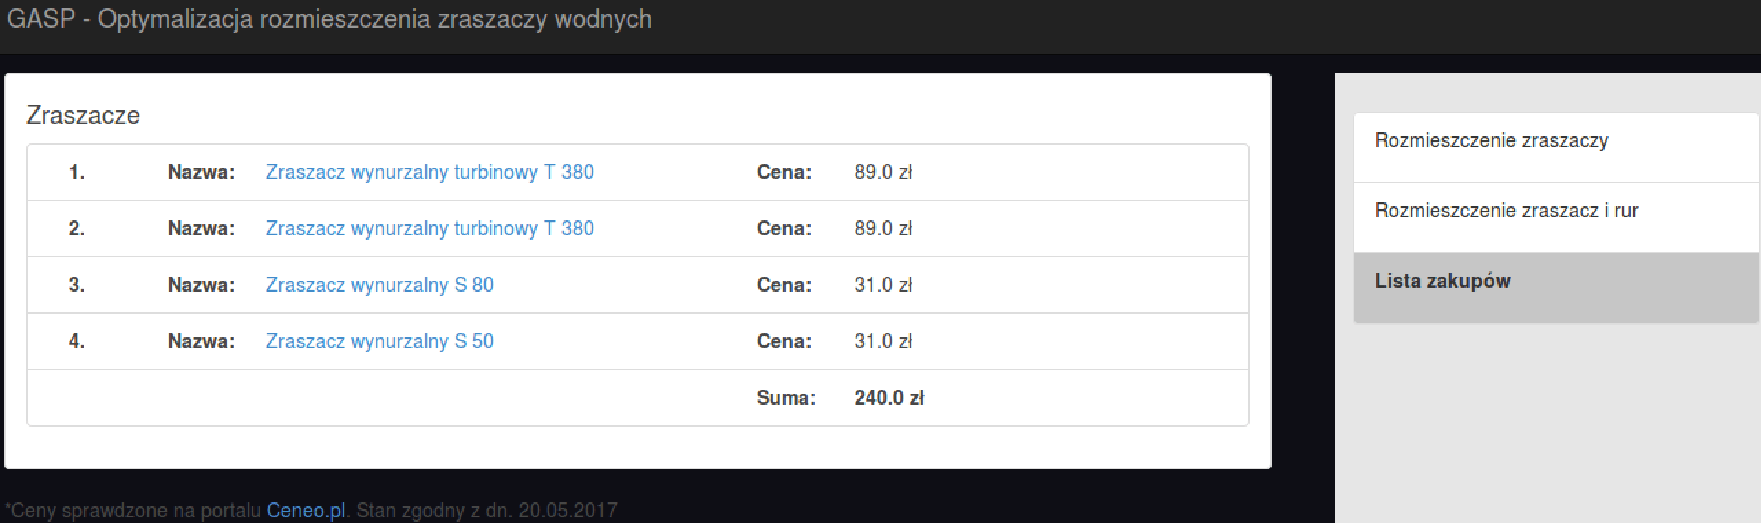
\includegraphics[ clip, scale=0.55]{gui_8}}
	\centering
	\caption{Lista zakupów}
	\label{fig:gui_8}
\end{figure}
\section{Porównanie algorytmów genetycznych}
\subsection{Cel badań}
Celem badań było sprawdzenie w jakim stopniu wybrane algorytmy genetyczne sprawdzą się w kontekście sformułowanego w pracy problemu oraz porównanie tych algorytmów ze sobą korzystając z zdefiniowanych w późniejszym podrozdziale przypadków testowych. Ponadto założono również jak cel ocenę przydatności wybranych algorytmów w opracowanym systemie wspomagania decyzji biorąc pod uwagę jakość generowanych rozwiązań oraz złożoność czasową.
\subsection{Plan badań}
Złożoność oceny algorytmów służących do optymalizacji wielokryterialnej jest znacznie większa niż tej dla algorytmów rozwiązujących problemy obejmujące jedno kryterium \cite{comparison_deb}. Wynika to z samej definicji rozwiązania problemu wielokryterialnego, która wyjaśniona została wcześniej. Oceniając rozwiązanie takiego problemu należy wziąć pod uwagę następujące składowe \cite{comparison_2}:\\
\begin{itemize}
	\item Dystans znalezionego niezdominowanego zbioru rozwiązań od prawdziwego zbioru Pareto.
	\item Równomierny rozkład znalezionych rozwiązań.
	\item Długość znalezionego frontu rozwiązań.
	\item Czas wykonania algorytmu.\\
\end{itemize}
Na potrzeby analizy i oceny dwóch zaproponowanych algorytmów wybrane zostały cztery metryki \cite{comparison_deb}\cite{comparison_2}:\\
\begin{enumerate}
	\item \textit{Współczynnik błędu (ER):} wskazuje procent rozwiązań, które nie należą do prawdziwego zbioru Pareto.
	\begin{equation}
		ER = \dfrac{\sum_{i=1}^{n} e_{i}}{n}
	\end{equation}
	, gdzie $n$ jest liczbą znalezionych niezdominowanych rozwiązań; $e_{i}$ zmienną określającą czy dane rozwiązanie znajduje się w prawdziwym zbiorze Pareto. Jeśli $e_{i} = 0$ rozwiązanie znajduje się w prawdziwym zbiorze Pareto, w przeciwnym razie $e_{i} = 1$. $ER = 0$ oznacza idealne rozwiązanie.\\
	\item \textit{Równomierny rozkład (SP):} metoda mierząca wariancję dystansu sąsiadujących rozwiązań znajdujących się na znalezionym froncie Pareto.
	\begin{equation}
		\begin{split}
		SP = \sqrt{\dfrac{1}{n-1}\sum_{i=1}^{n}{(\overline{d} - d_{i})}^{2}}\\
		d_{i} = \min_{i,j \neq i} \bigg{(} \sum_{k=1}^{K}|f_{i}^{k} - f_{j}^{k}|\bigg{)}
		\end{split}
	\end{equation}
	, gdzie $n$ jest liczbą znalezionych niezdominowanych rozwiązań; $\overline{d}$ jest wartością oznaczającą średni dystans pomiędzy rozwiązaniami. $f_{i}^{k}$ jest wartością $i$-tego rozwiązania z perspektywy kryterium $k$; $K$ jest liczbą wszystkich kryteriów; Wartość $SP = 0$ oznacza, że znalezione rozwiązania są rozłożone równomiernie.\\
	\item \textit{Jakość ogólna (GD):}  wskazuje jak daleko od prawdziwego zbioru Pareto znajduje się zbiór znalezionych niezdominowanych rozwiązań. Miara zdefiniowana w następujący sposób:
	\begin{equation}
		GD = \dfrac{\sqrt{\sum_{i=1}^{n} d_{i}^{2}}}{n}
	\end{equation}
	, gdzie $n$ oznacza liczbę znalezionych niezdominowanych rozwiązań; $d_{i}$ jest dystansem Euklidesowym pomiędzy danym rozwiązaniem, a najbliższym rozwiązaniem należącym do prawdziwego frontu Pareto. Wartość $DG = 0$ oznacza, że wszystkie znalezione rozwiązania leżą na prawdziwym froncie Pareto.\\
	\item \textit{Długość frontu (FE):} metoda wskazująca jak długi front został wygenerowany przez daną symulację.
	\begin{equation}	
		FE = \sqrt{\sum_{k=1}^{K} \max_{i, j \neq i} |f_{i}^{k} - f_{j}^{k}|}
	\end{equation}
	, gdzie $K$ oznacza liczbę funkcji celu; $f_{i}^{k}$ jest wartością $i$-tego rozwiązania z perspektywy kryterium $k$.\\
\end{enumerate}
Aby skorzystać z powyższych metryk konieczne było znalezienie prawdziwego frontu Pareto. Na potrzeby badań został on wygenerowany poprzez wybranie niezdominowanych rozwiązań ze skumulowanej puli rozwiązań powstałej na skutek uruchomienia każdego algorytmu 20 razy z wykorzystaniem 30 tysięcy pokoleń. Rezultaty każdej symulacji były dodawane do puli po czym zredukowane do rozwiązań niezdominowanych.

Do badań przygotowane zostały trzy przypadki testowe, a więc trzy różne obszary, które miały zostać nawodnione. Zostały one dobrane pod względem wielkości oraz kształtu, tak aby jak najlepiej zobrazować wpływ ograniczeń na działanie algorytmów.

W kolejnym podrozdziale zaprezentowany zostanie proces oraz rezultaty strojenia wybranych algorytmów. Następie opisane zostaną przeprowadzone badania. Dla każdego przypadku testowego każdy algorytm uruchamiany był dziesięć razy, tworząc pulę rozwiązań, z której wybierany były rozwiązania niezdominowane zilustrowane na wykresach.

Funkcje, których wartości przedstawione zostały na wykresach zaprezentowane i omówione zostały w rozdziale poświęconym modelowi matematycznemu.
\subsection{Strojenie algorytmów}
Jak zostało opisane wcześniej działanie algorytmów genetycznych opiera się na wielu parametrach. Parametry te są ze sobą mocno powiązane oraz znacząco wpływają na jakość symulacji. Proces doboru odpowiednich wartości dla wspomnianych parametrów, nazywa się strojeniem.

Przed przystąpieniem do badań konieczne jest odpowiednie nastrojenie wybranych algorytmów. Zostało to wykonane za pomocą metody iteracyjnej, działającej według następującego schematu:\\
\begin{enumerate}
	\item Ustaw wartości wszystkich parametrów na domyślne \eqref{default_params}.
	\item Wybierz pierwszy parametr mający zostać nastrojony oraz ustaw jego wartość na pierwszą z wybranych wartości testowych.
	\item Uruchom symulację oraz zapamiętaj wyniki.
	\item Jeśli używana wartość była ostatnią ze zbioru testowego porównaj zapamiętane rezultaty oraz wybierz wartość parametru dla której algorytm generował najlepsze rozwiązania. Jeśli w wybranym przedziale pozostały wartości wymagające sprawdzenie, wybierz kolejną wartość oraz przejdź do punktu 3.
	\item Wybierz kolejny parametr wymagający strojenia.\\
\end{enumerate}
\begin{table}[H]
\centering
\begin{tabular}{|l|c|c|}
\hline
\multicolumn{1}{|c|}{\textbf{Parametr}} & \textbf{Wartość domyślna} & \textbf{Wartości testowe}                    \\ \hline
Prawdopodobieństwo krzyżowania          & 0.9                       & 0.1, 0.2...1.0                             \\ \hline
Prawdopodobieństwo mutacji              & 0.05                      & 0.01, 0.02,...0.1, 0.2...0.5 \\ \hline
Wielkość turnieju                       & 2                         & 1, 2, 3, 4, 5                                    \\ \hline
Wielkość populacji - N                  & 100                       & 100, 200, 300, 400, 500                      \\ \hline
Wielkość populacji zewn. (SPEA)         & 1/4 N                     & 1 N, 1/2 N, 1/3 N...1/6 N                  \\ \hline
\end{tabular}
\caption{Domyślne oraz testowe wartości parametrów dla wybranych algorytmów genetycznych.}
\label{default_params}
\end{table}
Rozwiązania znalezione przez algorytmy były porównywane ze sobą za pomocą metryki zaproponowanej w \cite{tuning}. Pozwala ona porównać ze sobą dwa zbiory rozwiązań poprzez pokazanie w jakim stopniu rozwiązania z jednego zbioru są dominowane przez rozwiązania ze zbioru drugiego. Metryka jest zdefiniowana w następujący sposób:
\begin{equation}
	C(X^{'}, X^{''}) = \dfrac{|\{a^{''} \in X^{''}; \exists a^{'} \in X^{'}: a^{'} \preceq a^{''}\}|}{|X^{''}|}
\end{equation}
,gdzie $X^{'}, X^{''}$ są dwoma zbiorami biorącymi udział w porównaniu; $\preceq$ jest operatorem dominacji. $a^{'} \preceq a^{''}$ oznacza, że rozwiązanie $a^{'}$ ze zbioru $X^{'}$ dominuje rozwiązanie $a^{''}$ ze zbioru $X^{''}$.\\

Strojenie było wykonywane na drugim przypadku testowym przy generacji 500 pokoleń. Najlepsze wartości parametrów zostały przedstawione w tabeli \eqref{best_params}. Przy użyciu takich właśnie wartości przeprowadzono dalsze badania.

\begin{table}[H]
\centering
\begin{tabular}{|l|c|c|}
\hline
\multicolumn{1}{|c|}{\multirow{2}{*}{\textbf{Parametr}}} & \multicolumn{2}{c|}{\textbf{Wartość}} \\ \cline{2-3} 
\multicolumn{1}{|c|}{}                                   & NSGA-II            & SPEA             \\ \hline
Prawdopodobieństwo krzyżowania                           & 0.8                & 0.9              \\ \hline
Prawdopodobieństwo mutacji                               & 0.01               & 0.01             \\ \hline
Wielkość turnieju                                        & 2                  & 2                \\ \hline
Wielkość populacji - N                                   & 200                & 200              \\ \hline
Wielkość populacji zewn.                                 & -                  & 1/2 N            \\ \hline
\end{tabular}
\caption{Wybrane poprzez strojenie najlepsze wartości parametrów.}
\label{best_params}
\end{table}

\subsection{Badania}
\subsubsection{Pierwszy przypadek testowy - obszar mały}
Dla pierwszego, a więc najprostszego przypadku testowego \eqref{fig:small_area} algorytmy uruchamiane były w celu ewaluacji 1000 pokoleń. W trakcie symulacji zebrano również wyniki reprezentujące pokolenie 100 oraz 500, co zostało zobrazowane na wykresach \eqref{fig:small_front}.
\begin{figure}[H]
	\makebox[\textwidth]{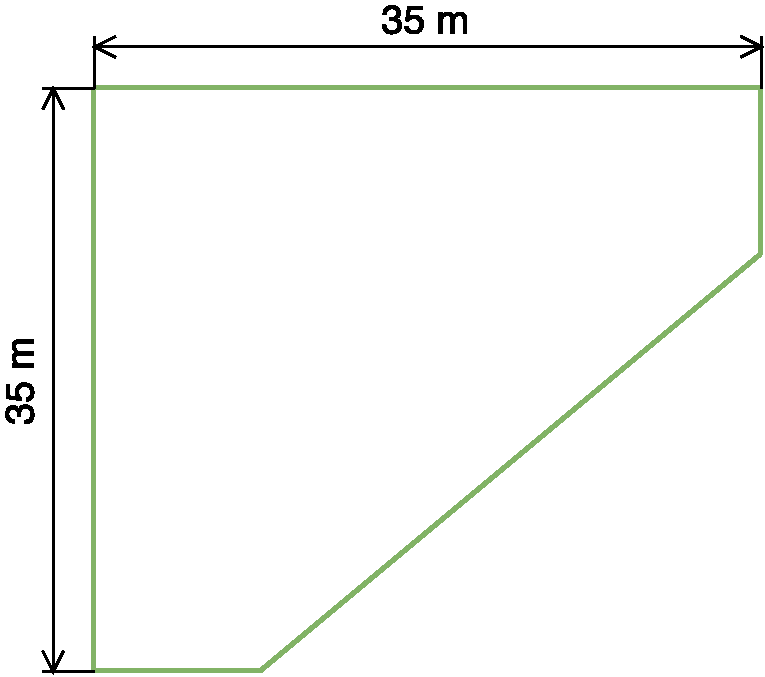
\includegraphics[ clip, scale=0.4]{small_area}}
	\centering
	\caption{Pierwszy przypadek testowy - obszar mały.}
	\label{fig:small_area}
\end{figure}
Analizując przedstawione wykresy można zauważyć, że oba algorytmy bardzo szybko osiągają front Pareto dla niskich wartości funkcji $F_{2}$. Dzieje się tak dlatego, że w tych przypadkach wykorzystywana jest mała liczba zraszaczy co znacząco zmniejsza złożoność problemu. Razem ze wzrostem wartości funkcji $F_{2}$ zwiększa się dystans pomiędzy znalezionymi rozwiązaniami, a tymi leżącymi na froncie Pareto, co dobrze widać na wykresie pokazującym wyniki po ewaluacji 100 pokoleń (\ref{fig:small_front}a). Obrazują to również wartości metryki $GD$ przedstawione w tabeli (\ref{fig:small_metrics}c). Warto tutaj zauważyć, że na tym etapie algorytm SPEA jest ponad trzy razy gorszy od NSGA-II jeśli chodzi o odległość znalezionych rozwiązań od rozwiązań optymalnych. \newpage
\begin{figure*}\centering
\subfloat[100 generacji\label{fig:small_pareto_100}]
        {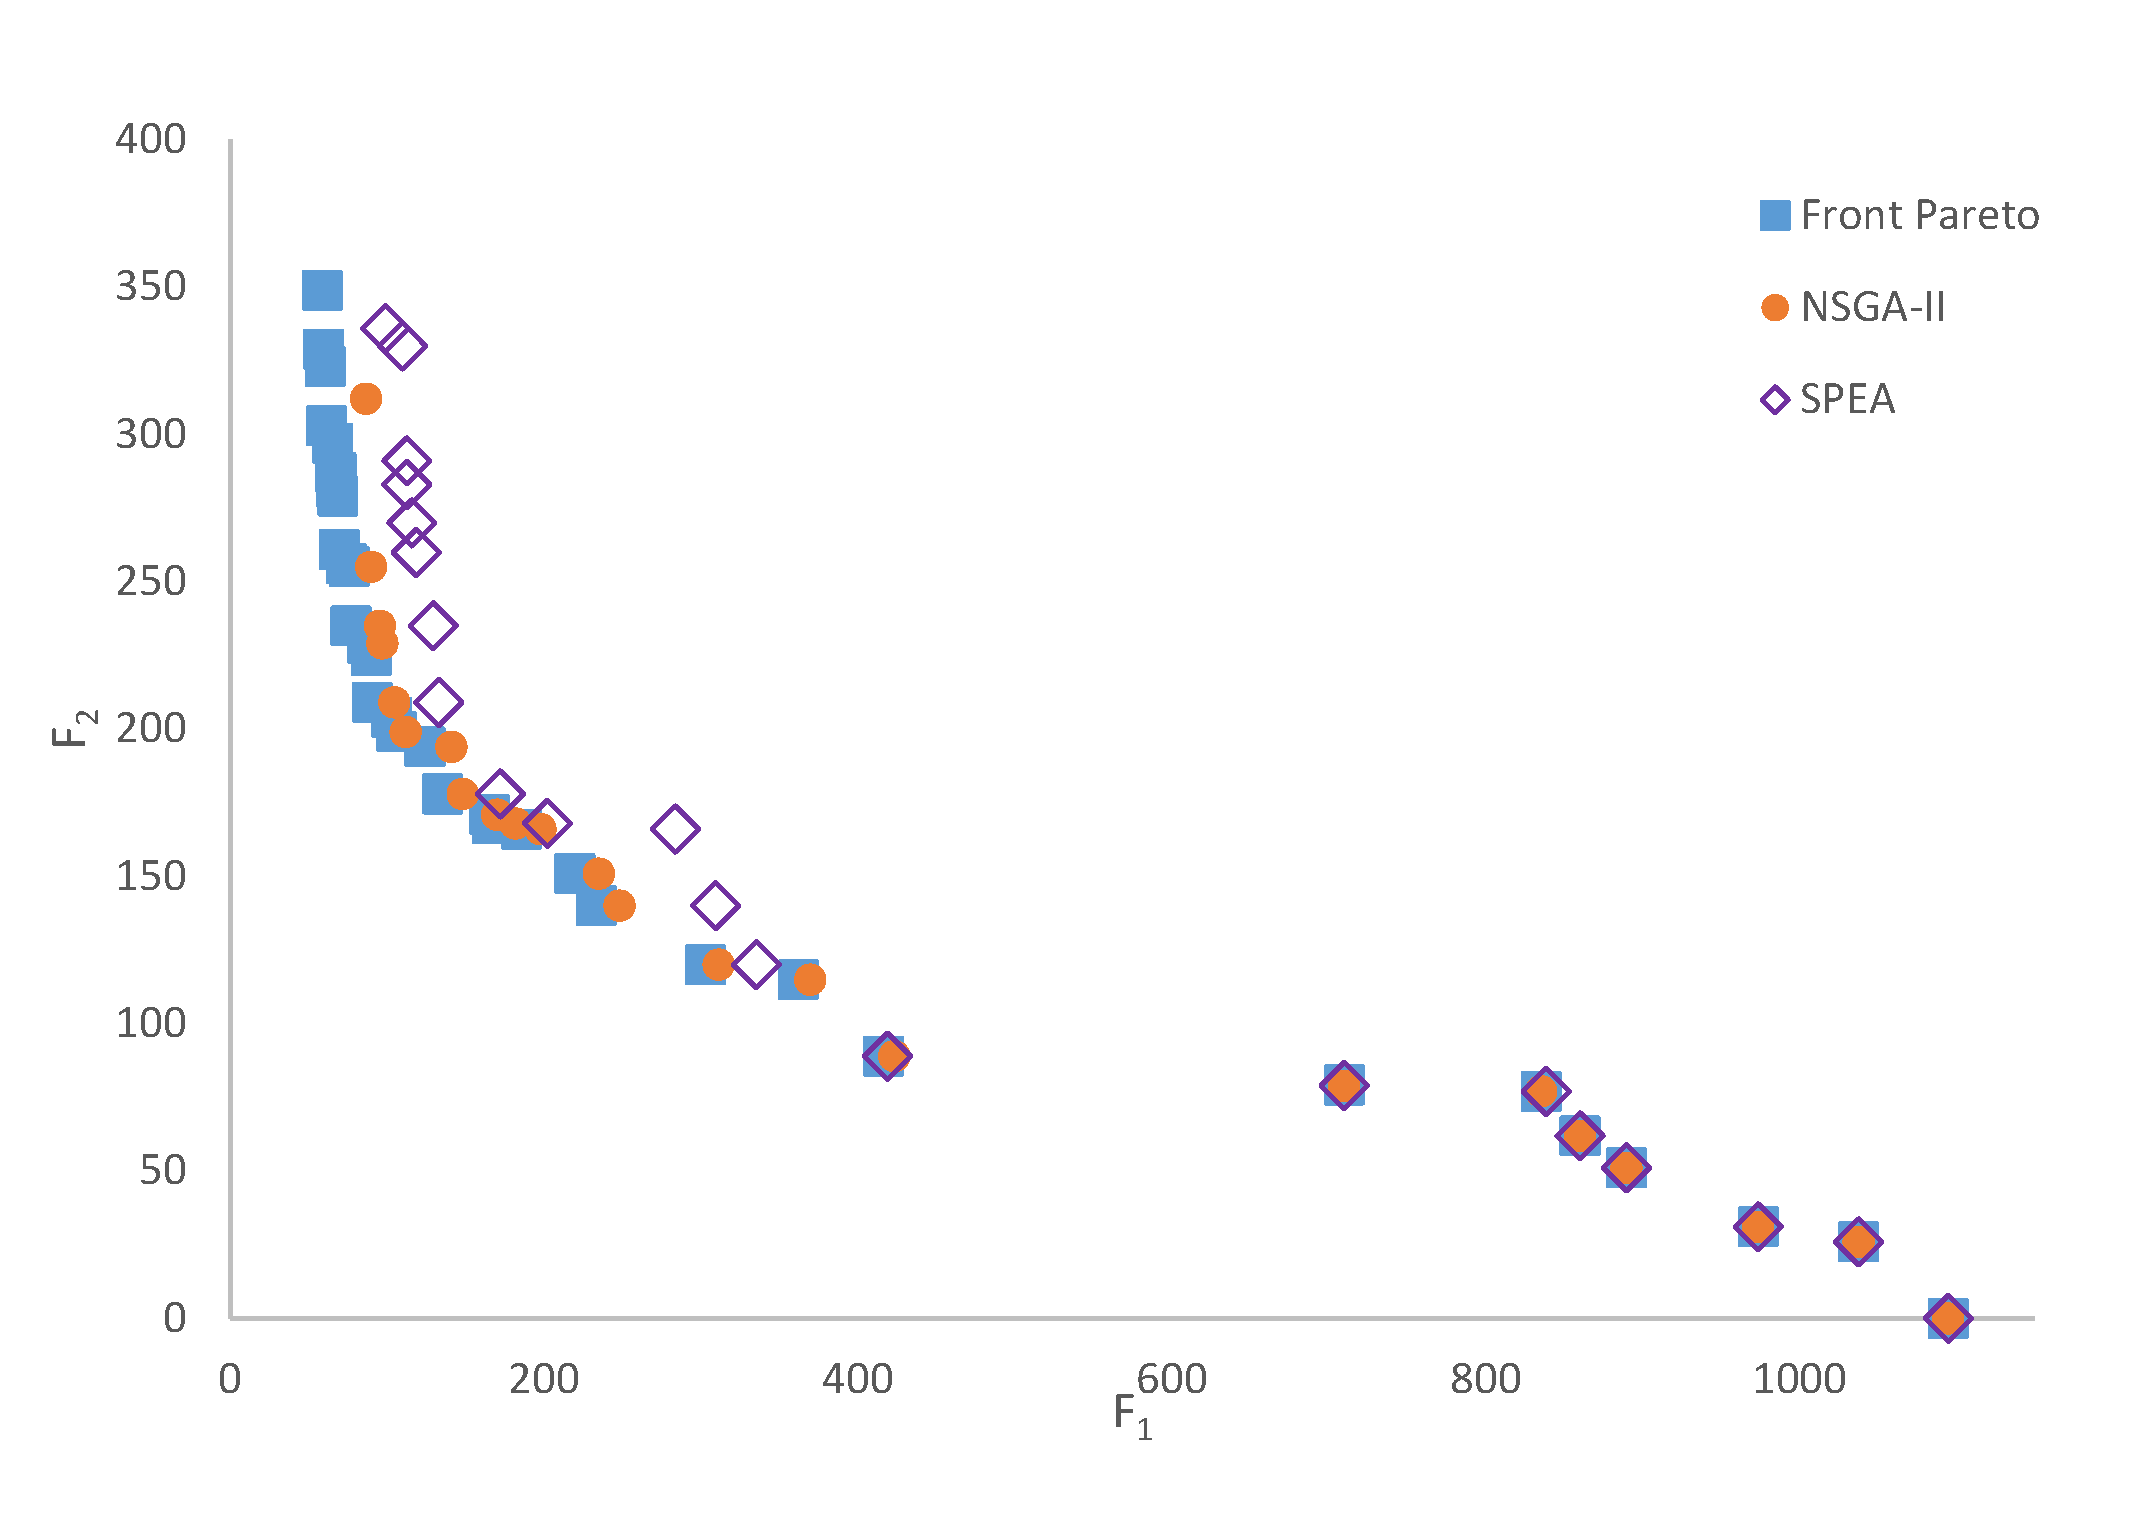
\includegraphics[width=0.5\textwidth]{small_pareto_100}}
    \hfill
\subfloat[500 generacji\label{fig:small_pareto_500}]
         {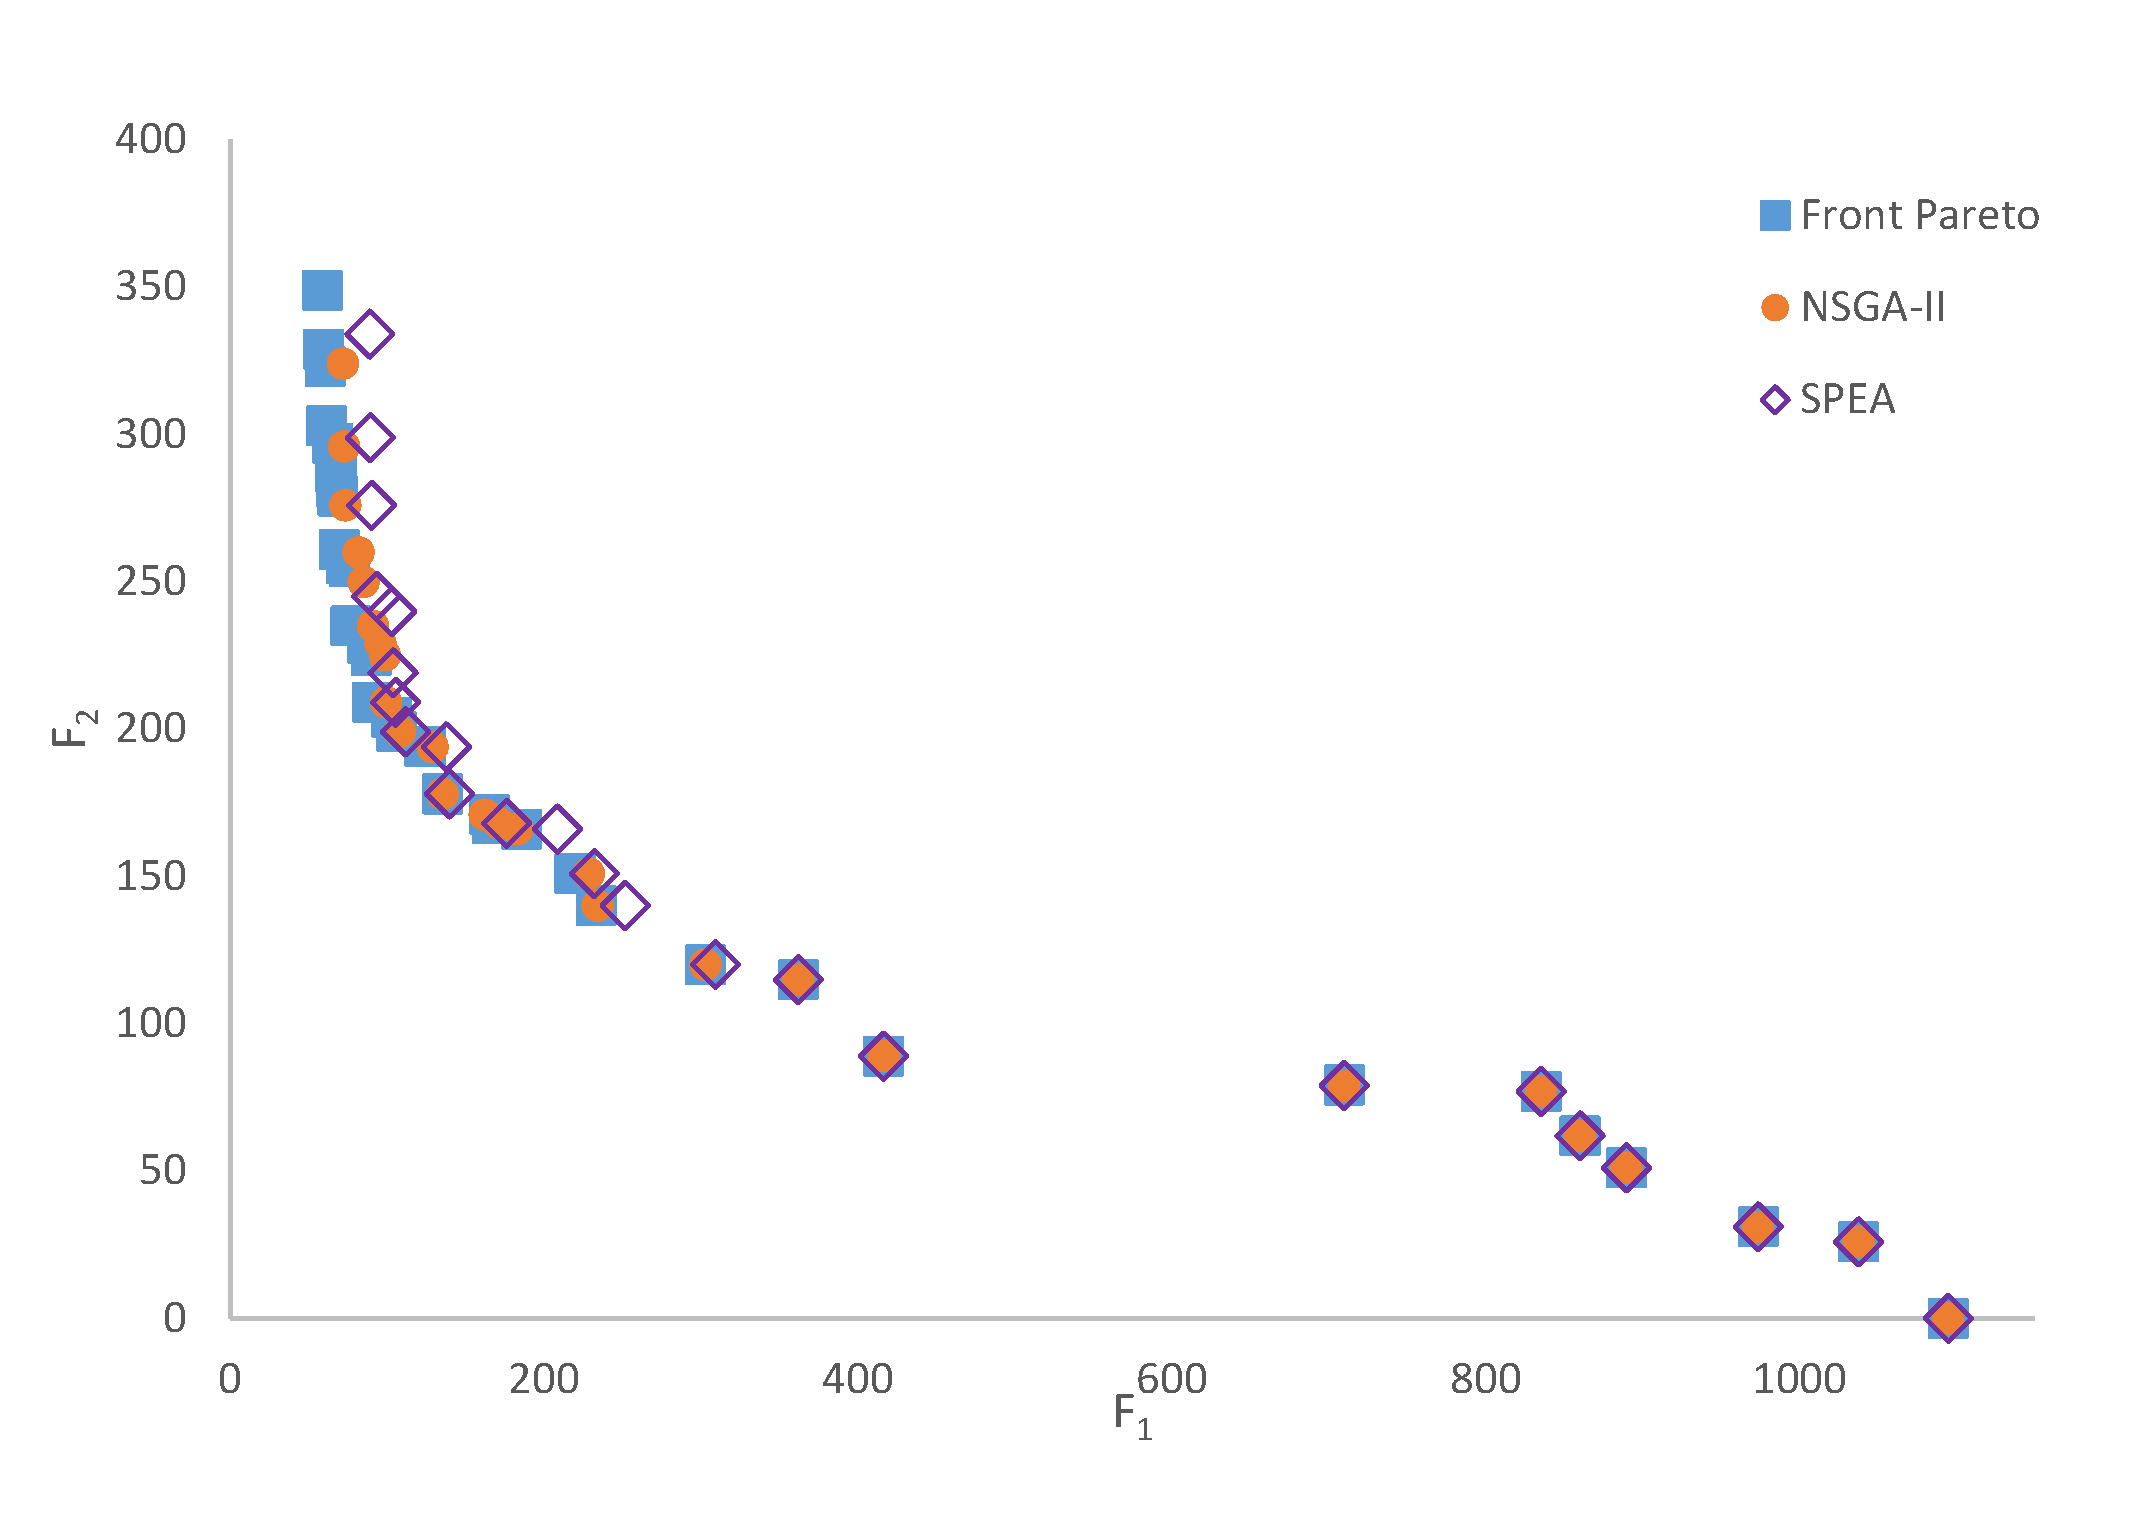
\includegraphics[width=0.5\textwidth]{small_pareto_500}}
    \hfill
\subfloat[1000 generacji\label{fig:small_pareto_1000}]
        {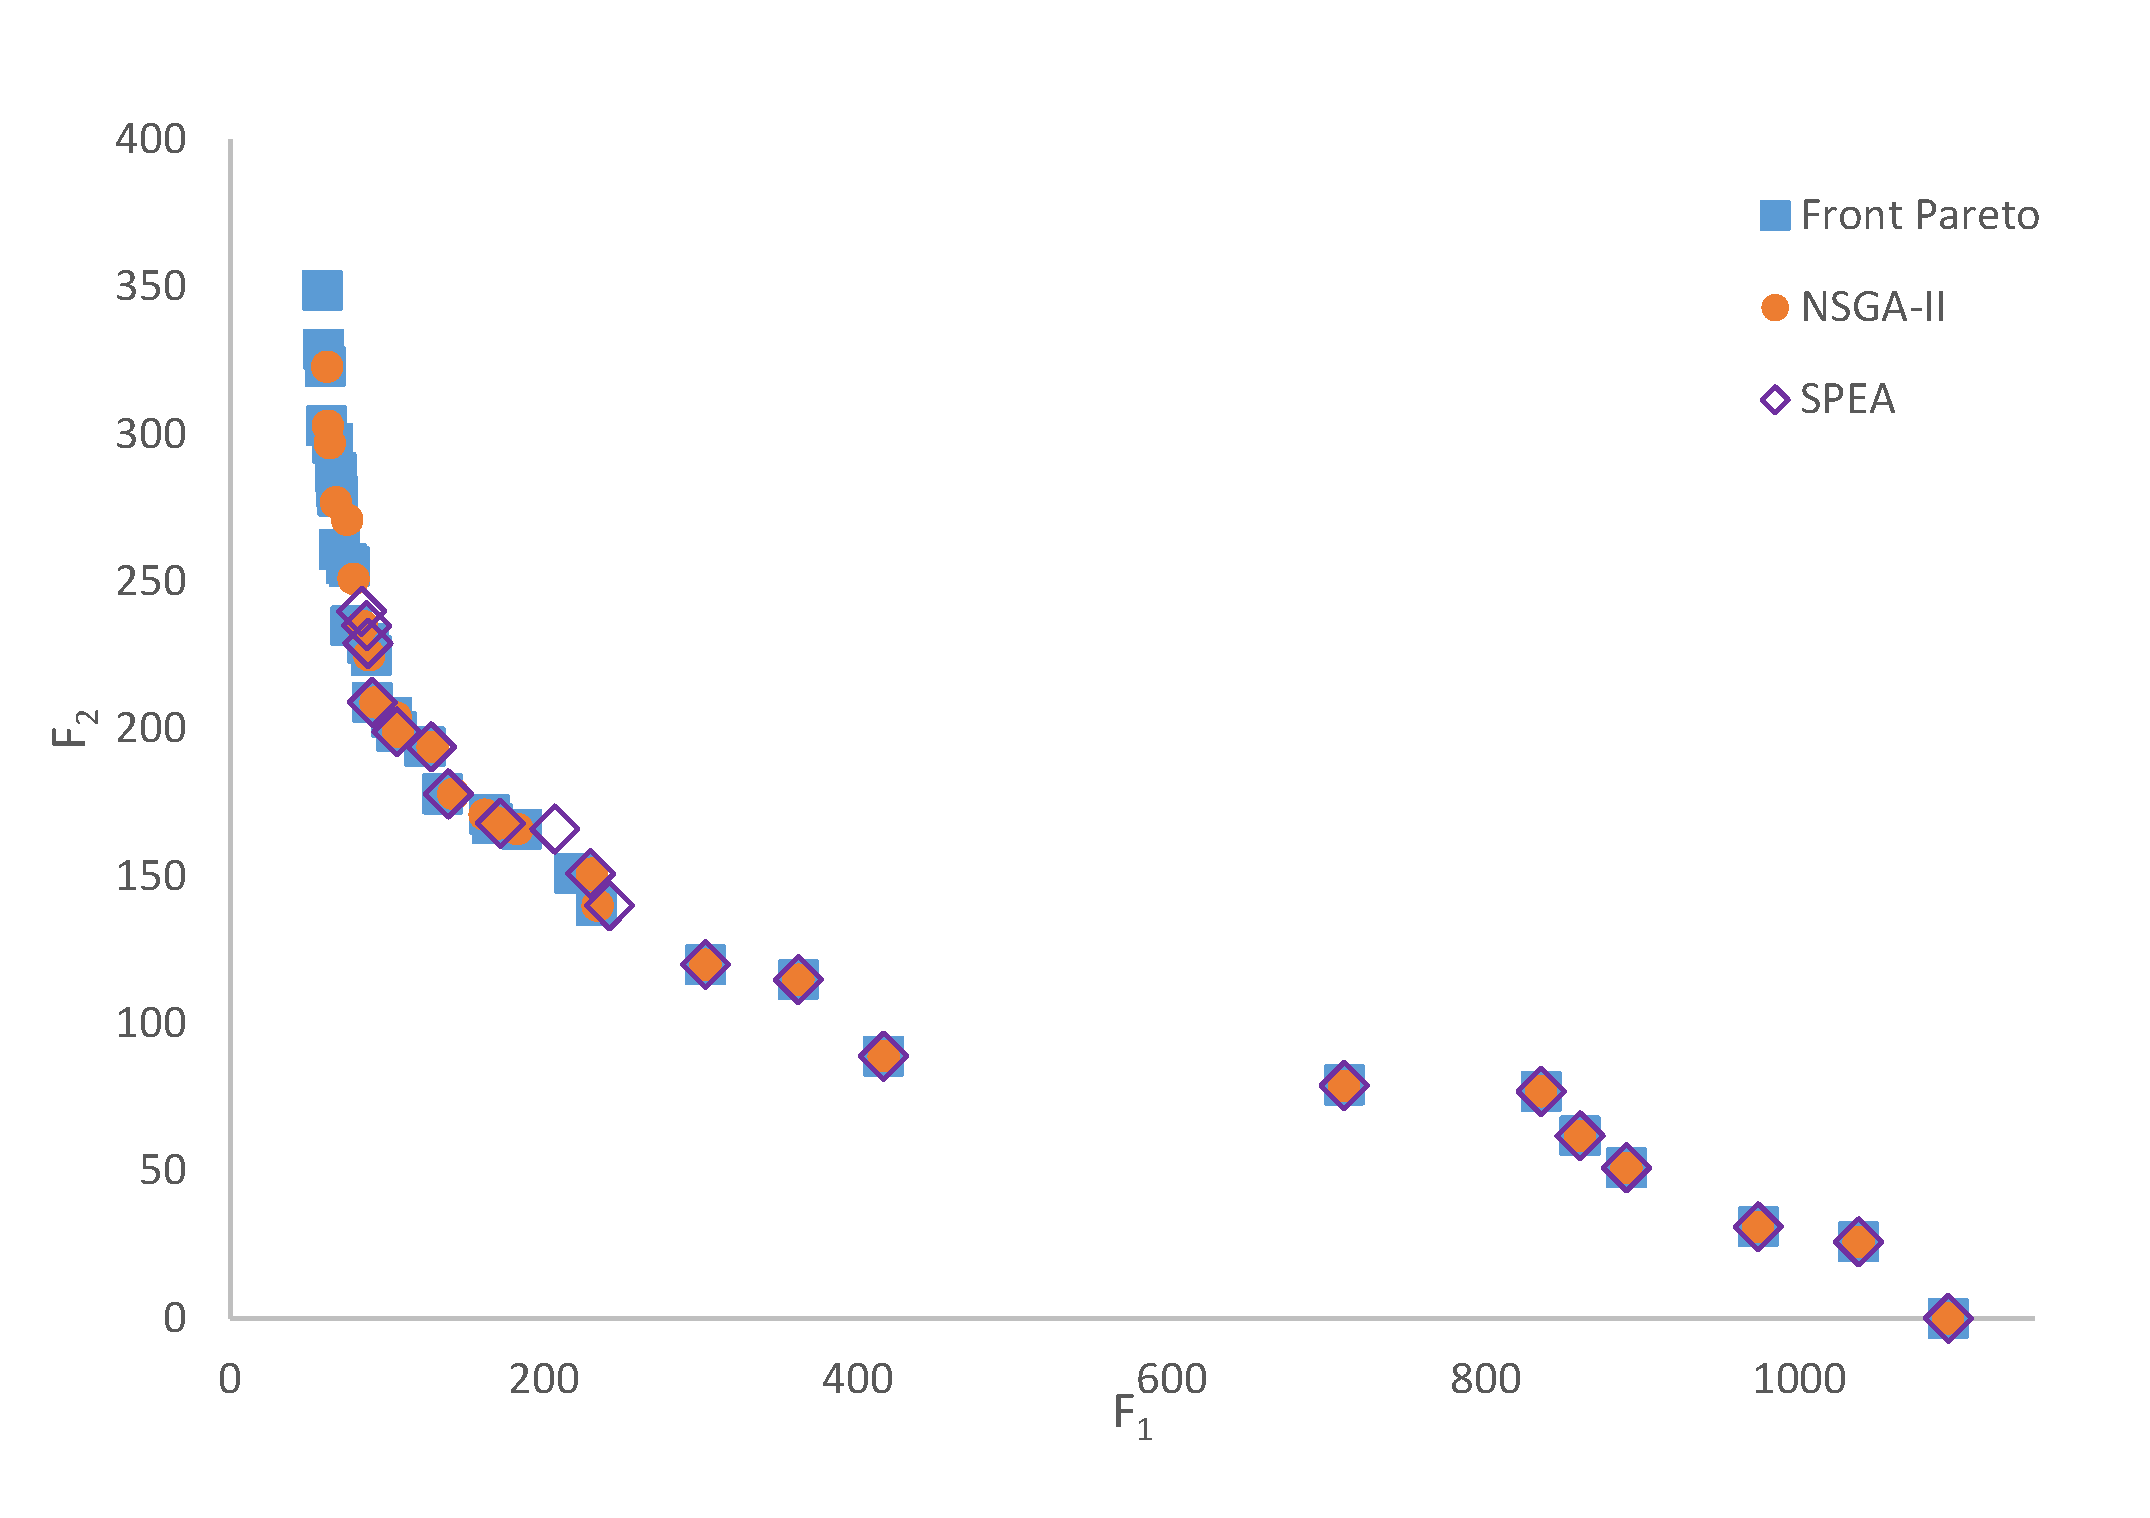
\includegraphics[width=0.5\textwidth]{small_pareto_1000}}
\caption{Rozwiązania niezdominowane otrzymane dla pierwszego przypadku testowego.}
    \label{fig:small_front}
\end{figure*}
Wraz z generowaniem nowych pokoleń znalezione rozwiązania niezdominowane coraz bardziej zbliżają się do frontu Pareto.

Obserwując wyniki symulacji oraz wartości metryk można zauważyć, że w pokoleniu 500. NSGA-II prezentuje się lepiej niemal we wszystkich aspektach: znalezione przez niego rozwiązania charakteryzują się mniejszym współczynnikiem błędu, wyznaczają dłuższy front oraz znajdują się bliżej frontu Pareto. Sytuacja wygląda inaczej jeśli chodzi o równomierność rozkładu ($SP$). W tym aspekcie lepiej wypadł algorytm SPEA.

Rozwiązania z 1000. generacji znajdują się zdecydowanie najbliżej rozwiązań optymalnych. Ciekawą obserwacją jest to, że w ostatnim pokoleniu wartość metryki $GD$ dla algorytmu SPEA jest gorsza niż wartość tej samej metryki dla algorytmu NSGA-II w pokoleniu 500. SPEA prezentuje się jednak lepiej, jeśli chodzi o wartość metryki definiującej współczynnik błędu - w porównaniu do liczby wszystkich rozwiązań niezdominowanych algorytm SPEA znalazł więcej rozwiązań leżących na froncie Pareto. W porównaniu do pokolenia 500. algorytm NSGA-II znacząco powiększył swoją przewagę, jeśli chodzi o długość wygenerowanego frontu.\newpage
\begin{figure*}\centering
\subfloat[Współczynnik błędu (ER)\label{fig:er_small}]
        {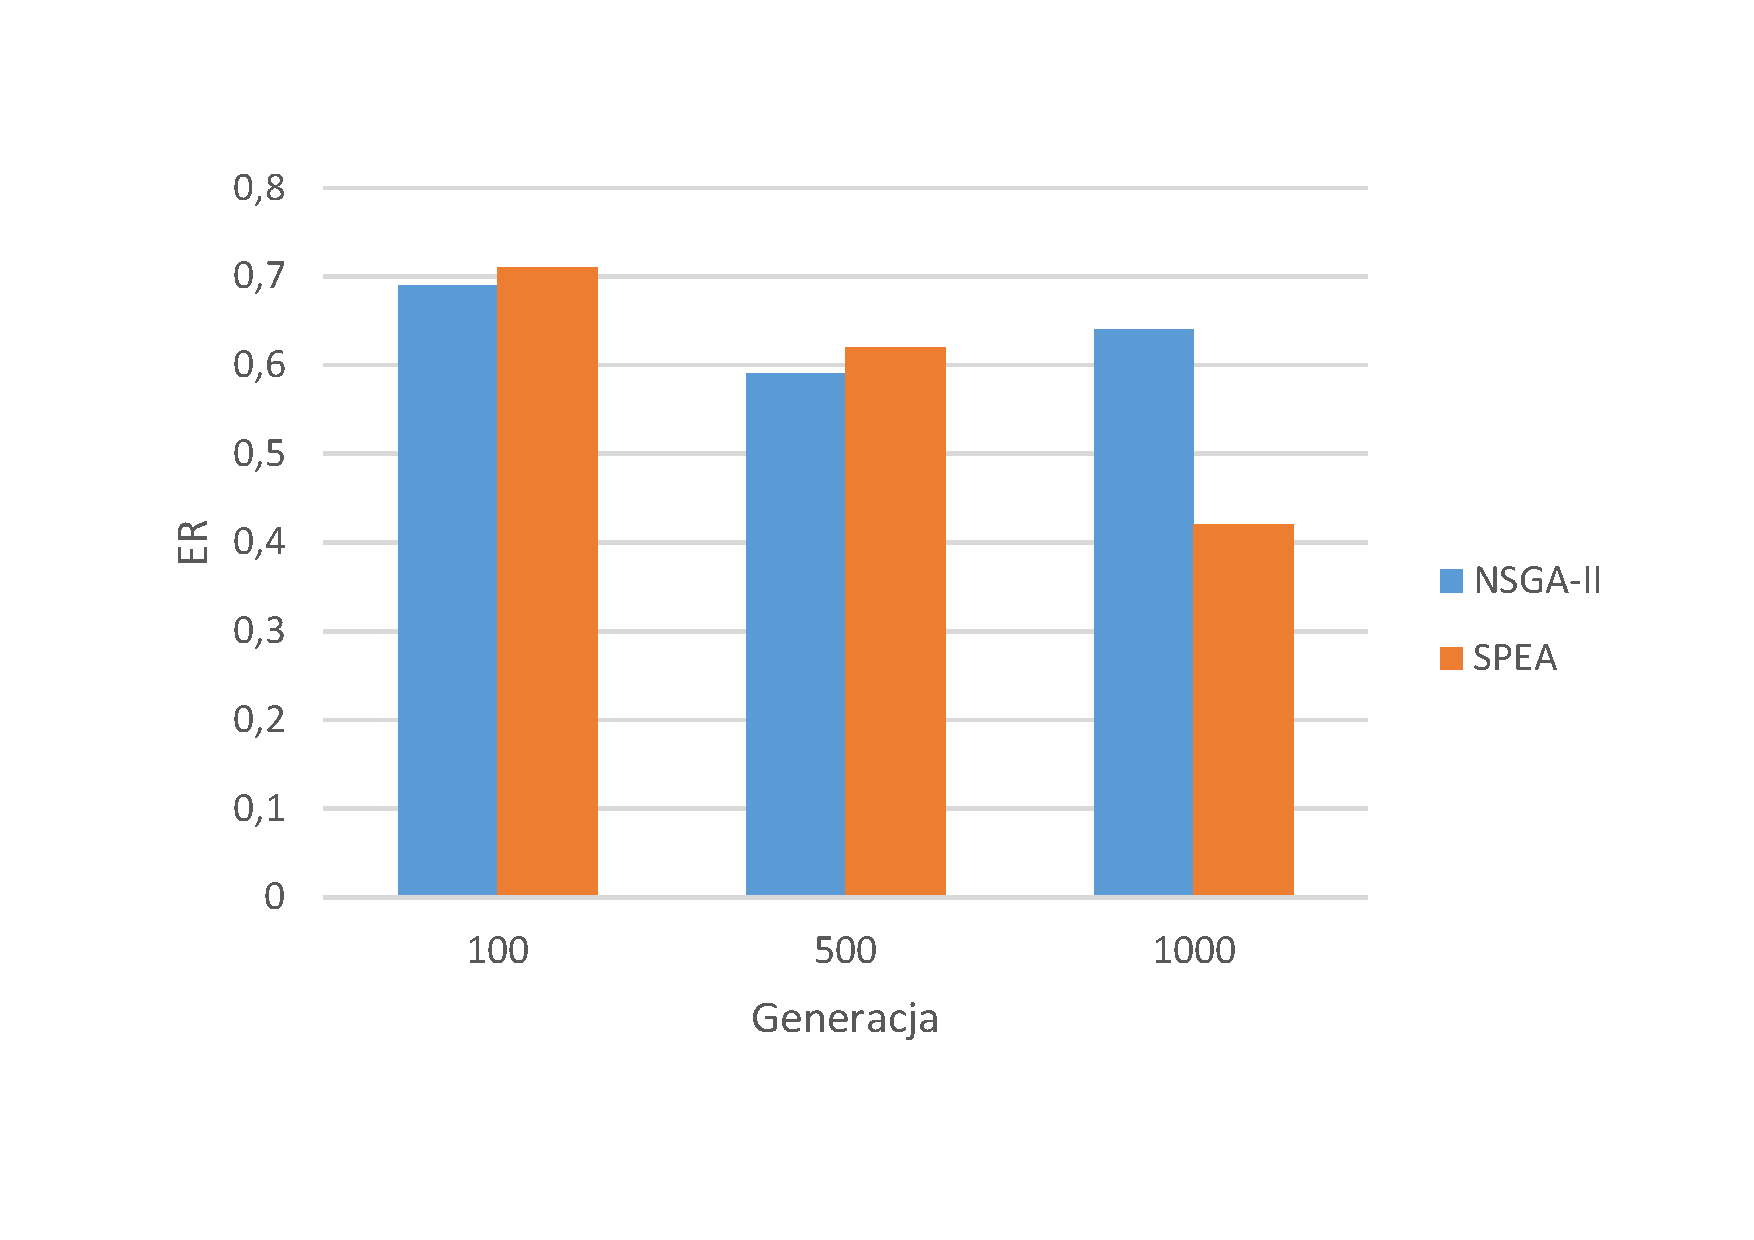
\includegraphics[width=0.5\textwidth]{er_small}}
    \hfill
\subfloat[Długość frontu (FE)\label{fig:fe_small}]
         {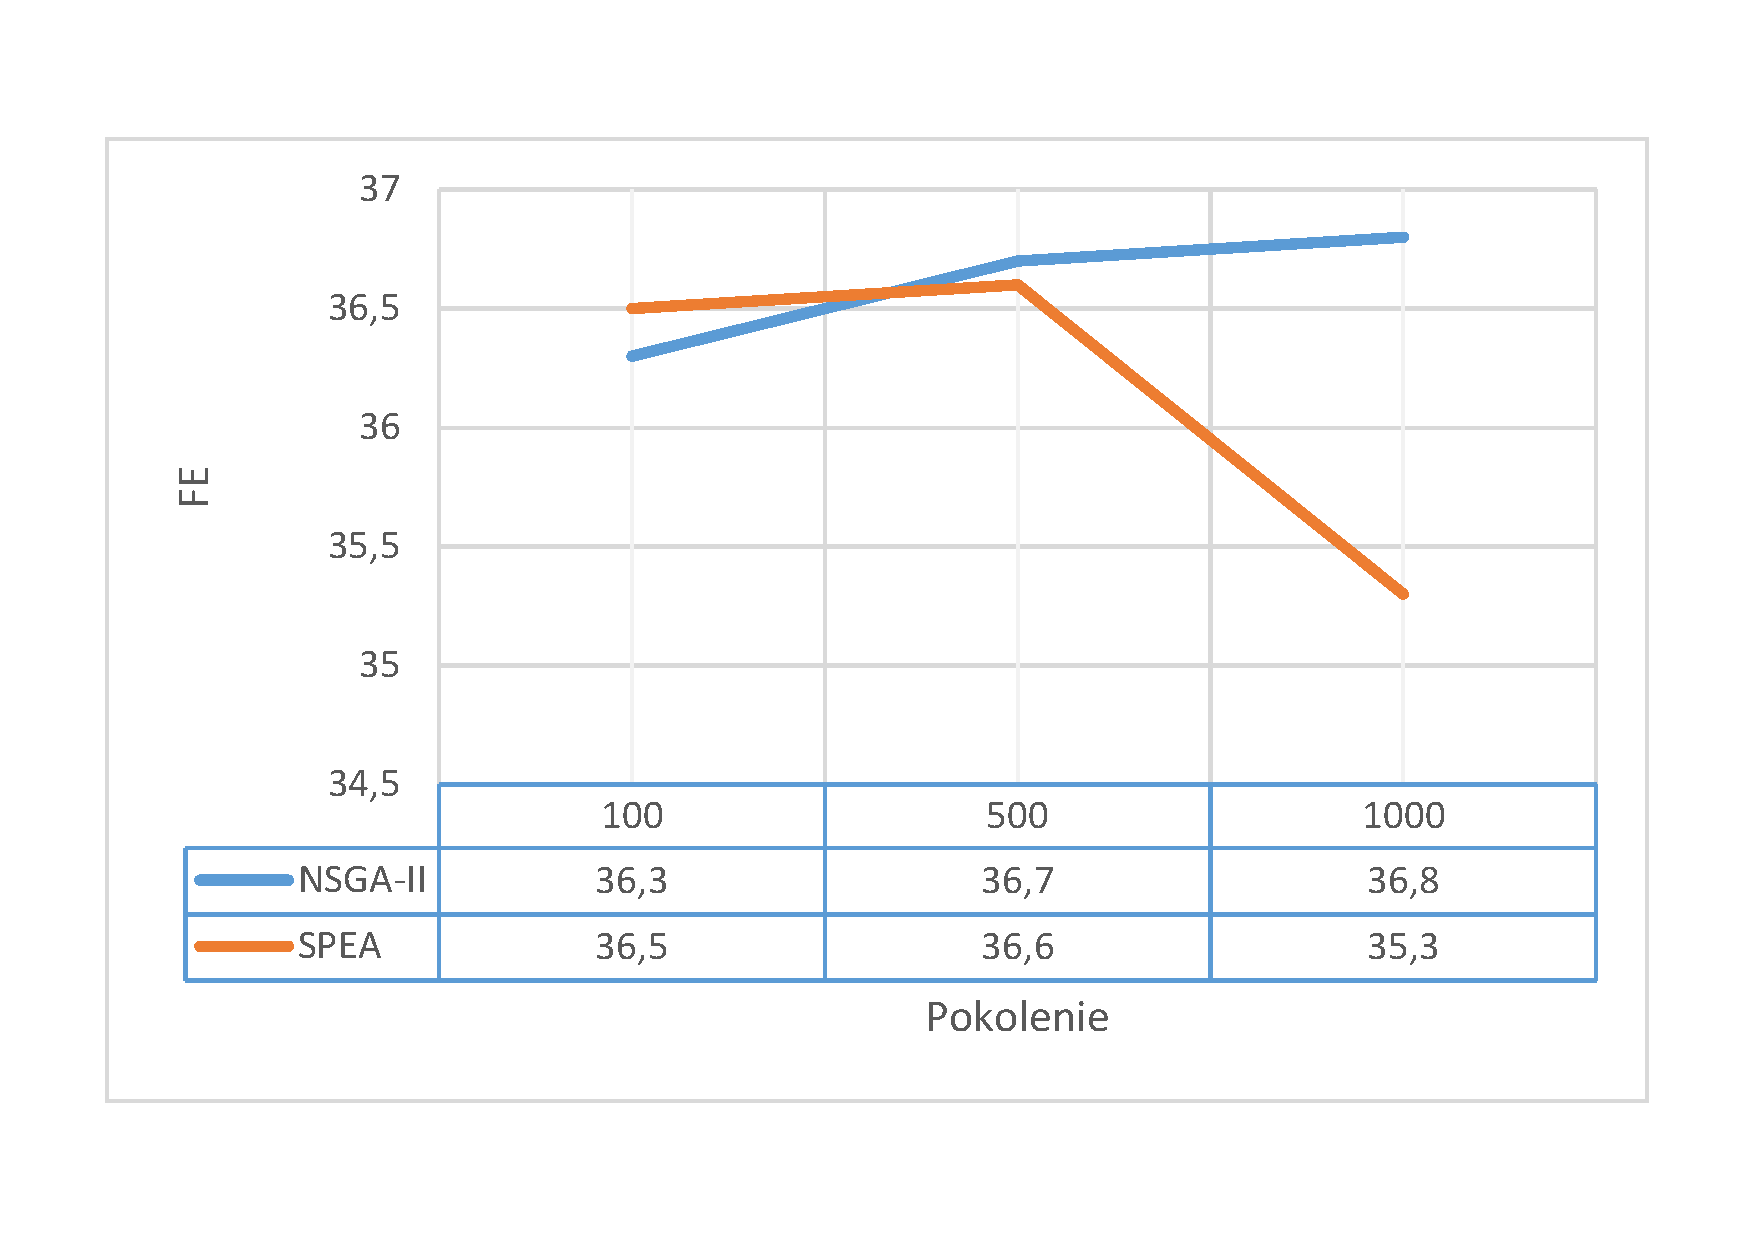
\includegraphics[width=0.5\textwidth]{fe_small}}

\subfloat[Jakość ogólna (GD)\label{fig:gd_small}]
         {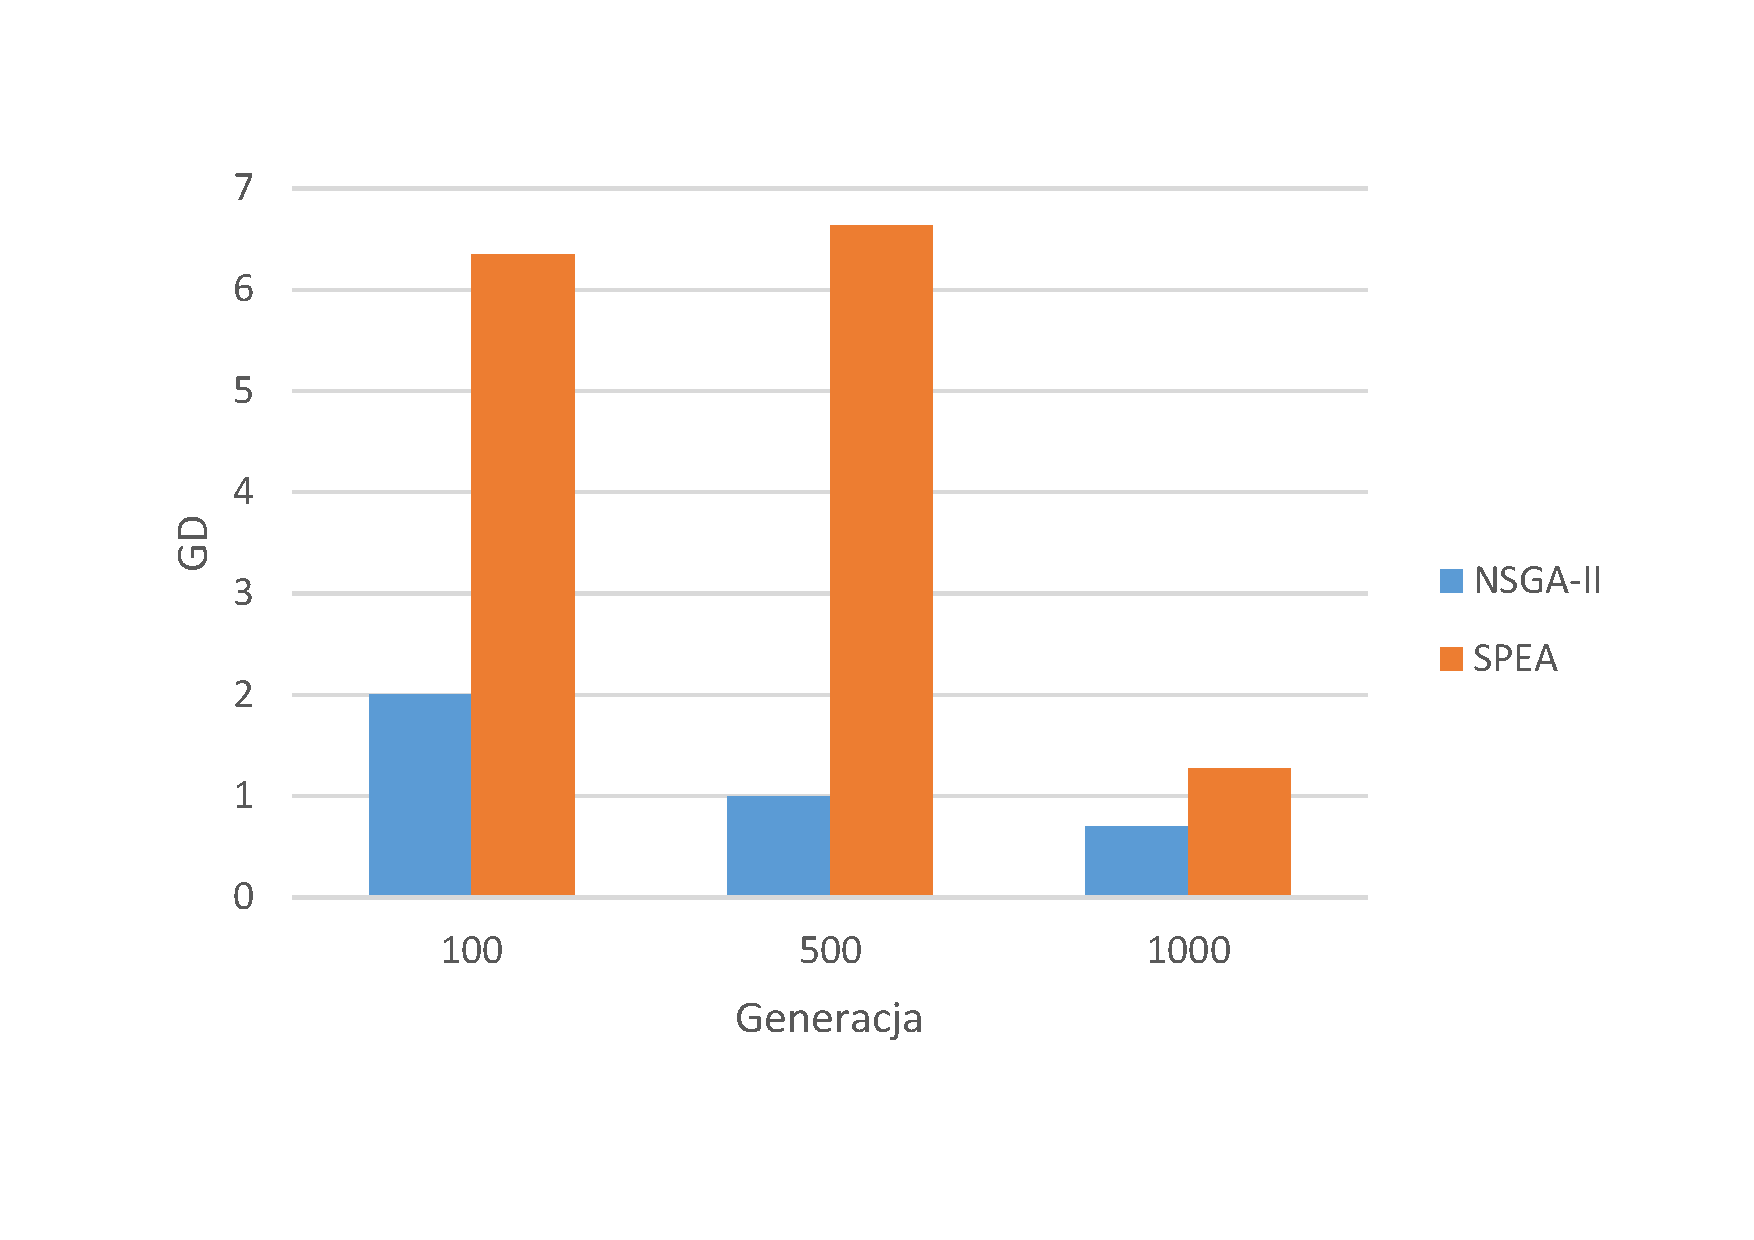
\includegraphics[width=0.5\textwidth]{gd_small}}
    \hfill
\subfloat[Równomierność rozkładu (SP)\label{fig:sp_small}]
        {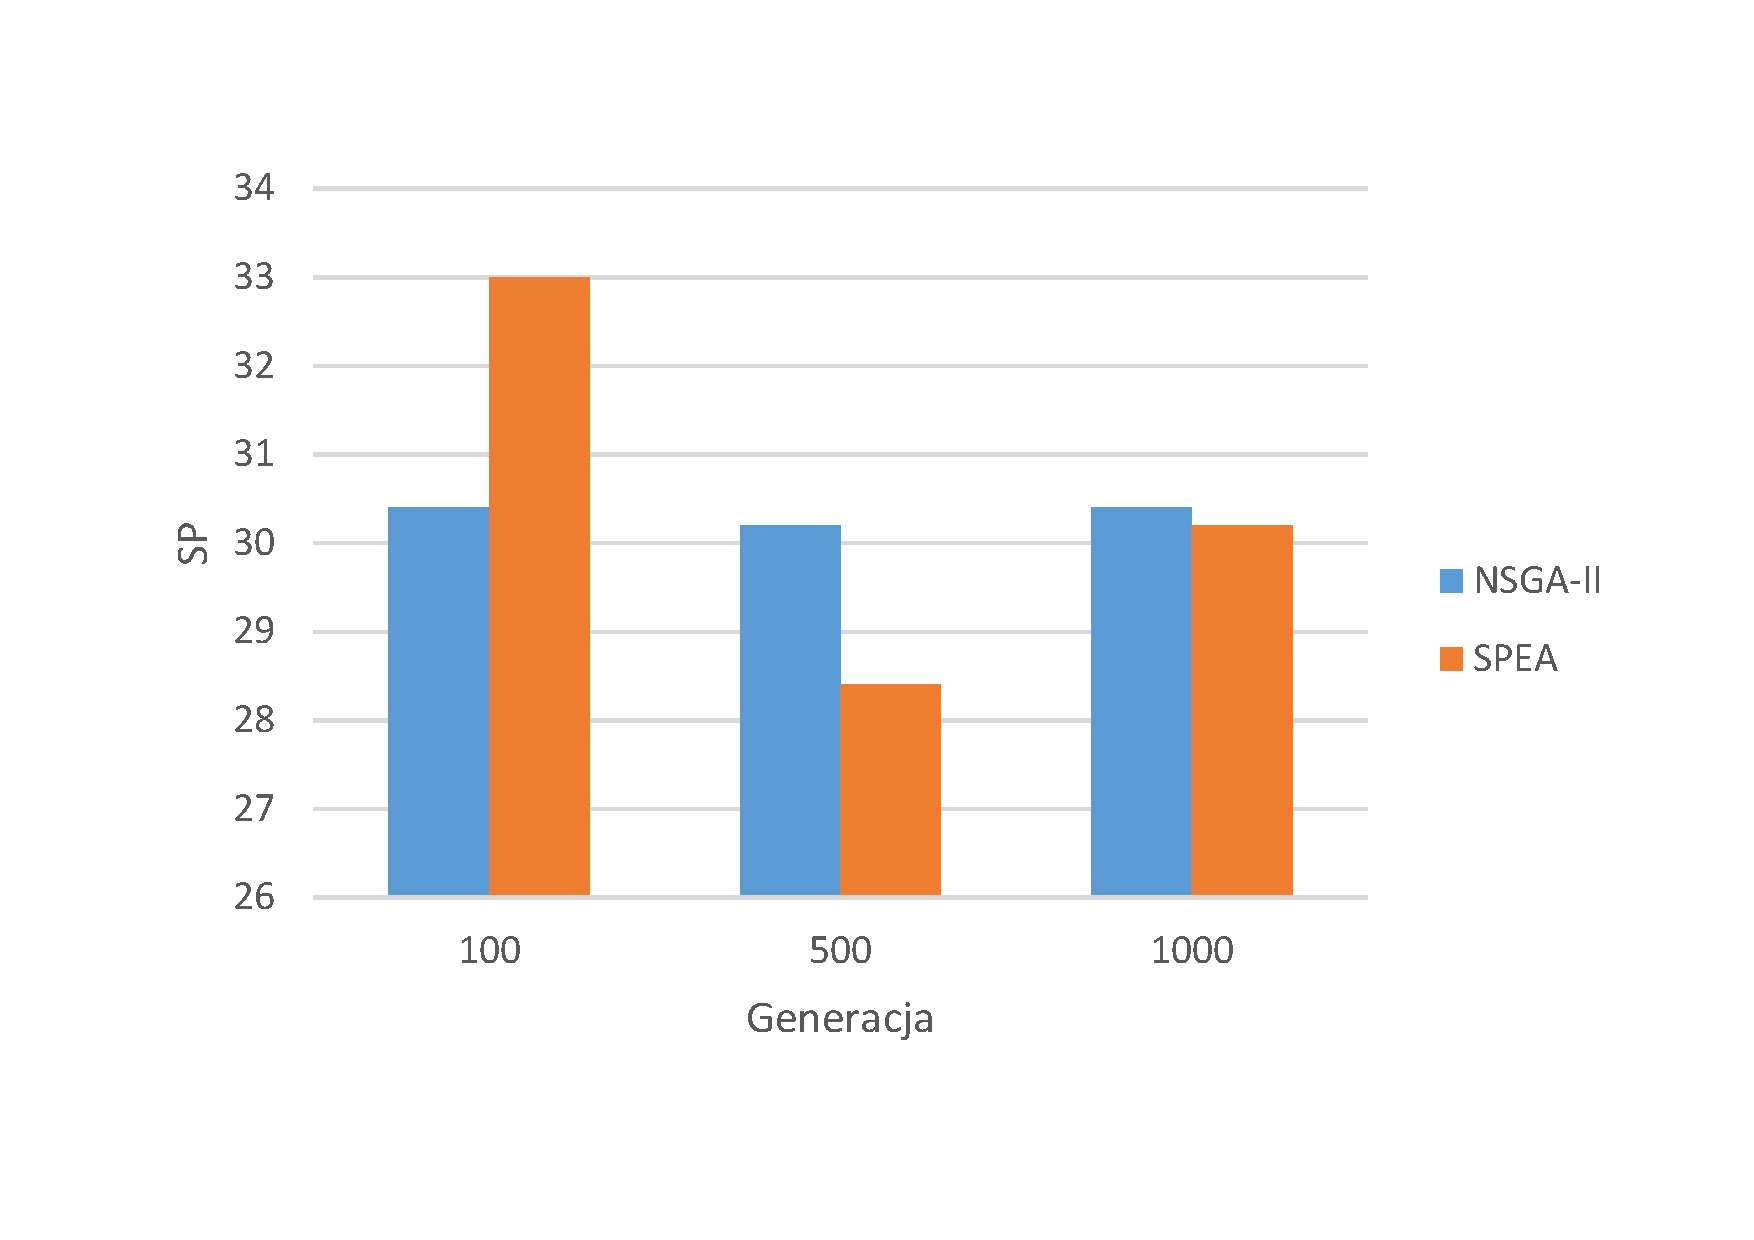
\includegraphics[width=0.5\textwidth]{sp_small}}
\caption{Wartość metryk charakteryzujących wyniki symulacji dla pierwszego przypadku testowego.}
    \label{fig:small_metrics}
\end{figure*}
Podsumowując, z pierwszym przypadkiem testowym oba algorytmy poradziły sobie dobrze. NSGA-II znalazł więcej rozwiązań niezdominowanych. Co więcej rozwiązania te znajdowały się bliżej frontu Pareto niż rozwiązania znalezione przez algorytm SPEA. Poza tym NSGA-II wygenerował znacząco dłuższy front.

Z drugiej strony algorytm SPEA znalazł więcej rozwiązań znajdujących się na froncie Pareto co określa metryka $ER$. Ponadto rozwiązania znalezione przez SPEA charakteryzowały się większą równomiernością rozkładu.\newpage
\subsubsection{Drugi przypadek testowy - obszar średni}
W celu zbadania działania wybranych algorytmów dla drugiego przypadku testowego \eqref{fig:medium_area} wygenerowano 2000 generacji. Ponadto odnotowano wyniki z 100, 500 oraz 1000 pokolenia.
\begin{figure}[H]
	\makebox[\textwidth]{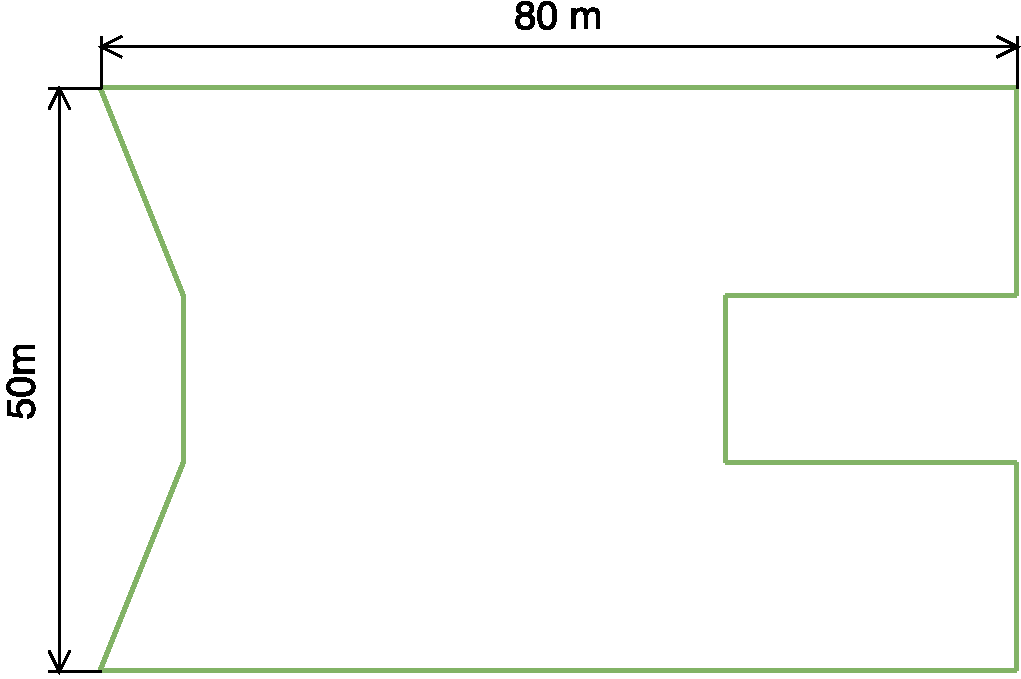
\includegraphics[ clip, scale=0.4]{medium_area}}
	\centering
	\caption{Drugi przypadek testowy - obszar średni.}
	\label{fig:medium_area}
\end{figure}
\begin{figure*}\centering
\subfloat[100 generacji\label{fig:medium_pareto_100}]
        {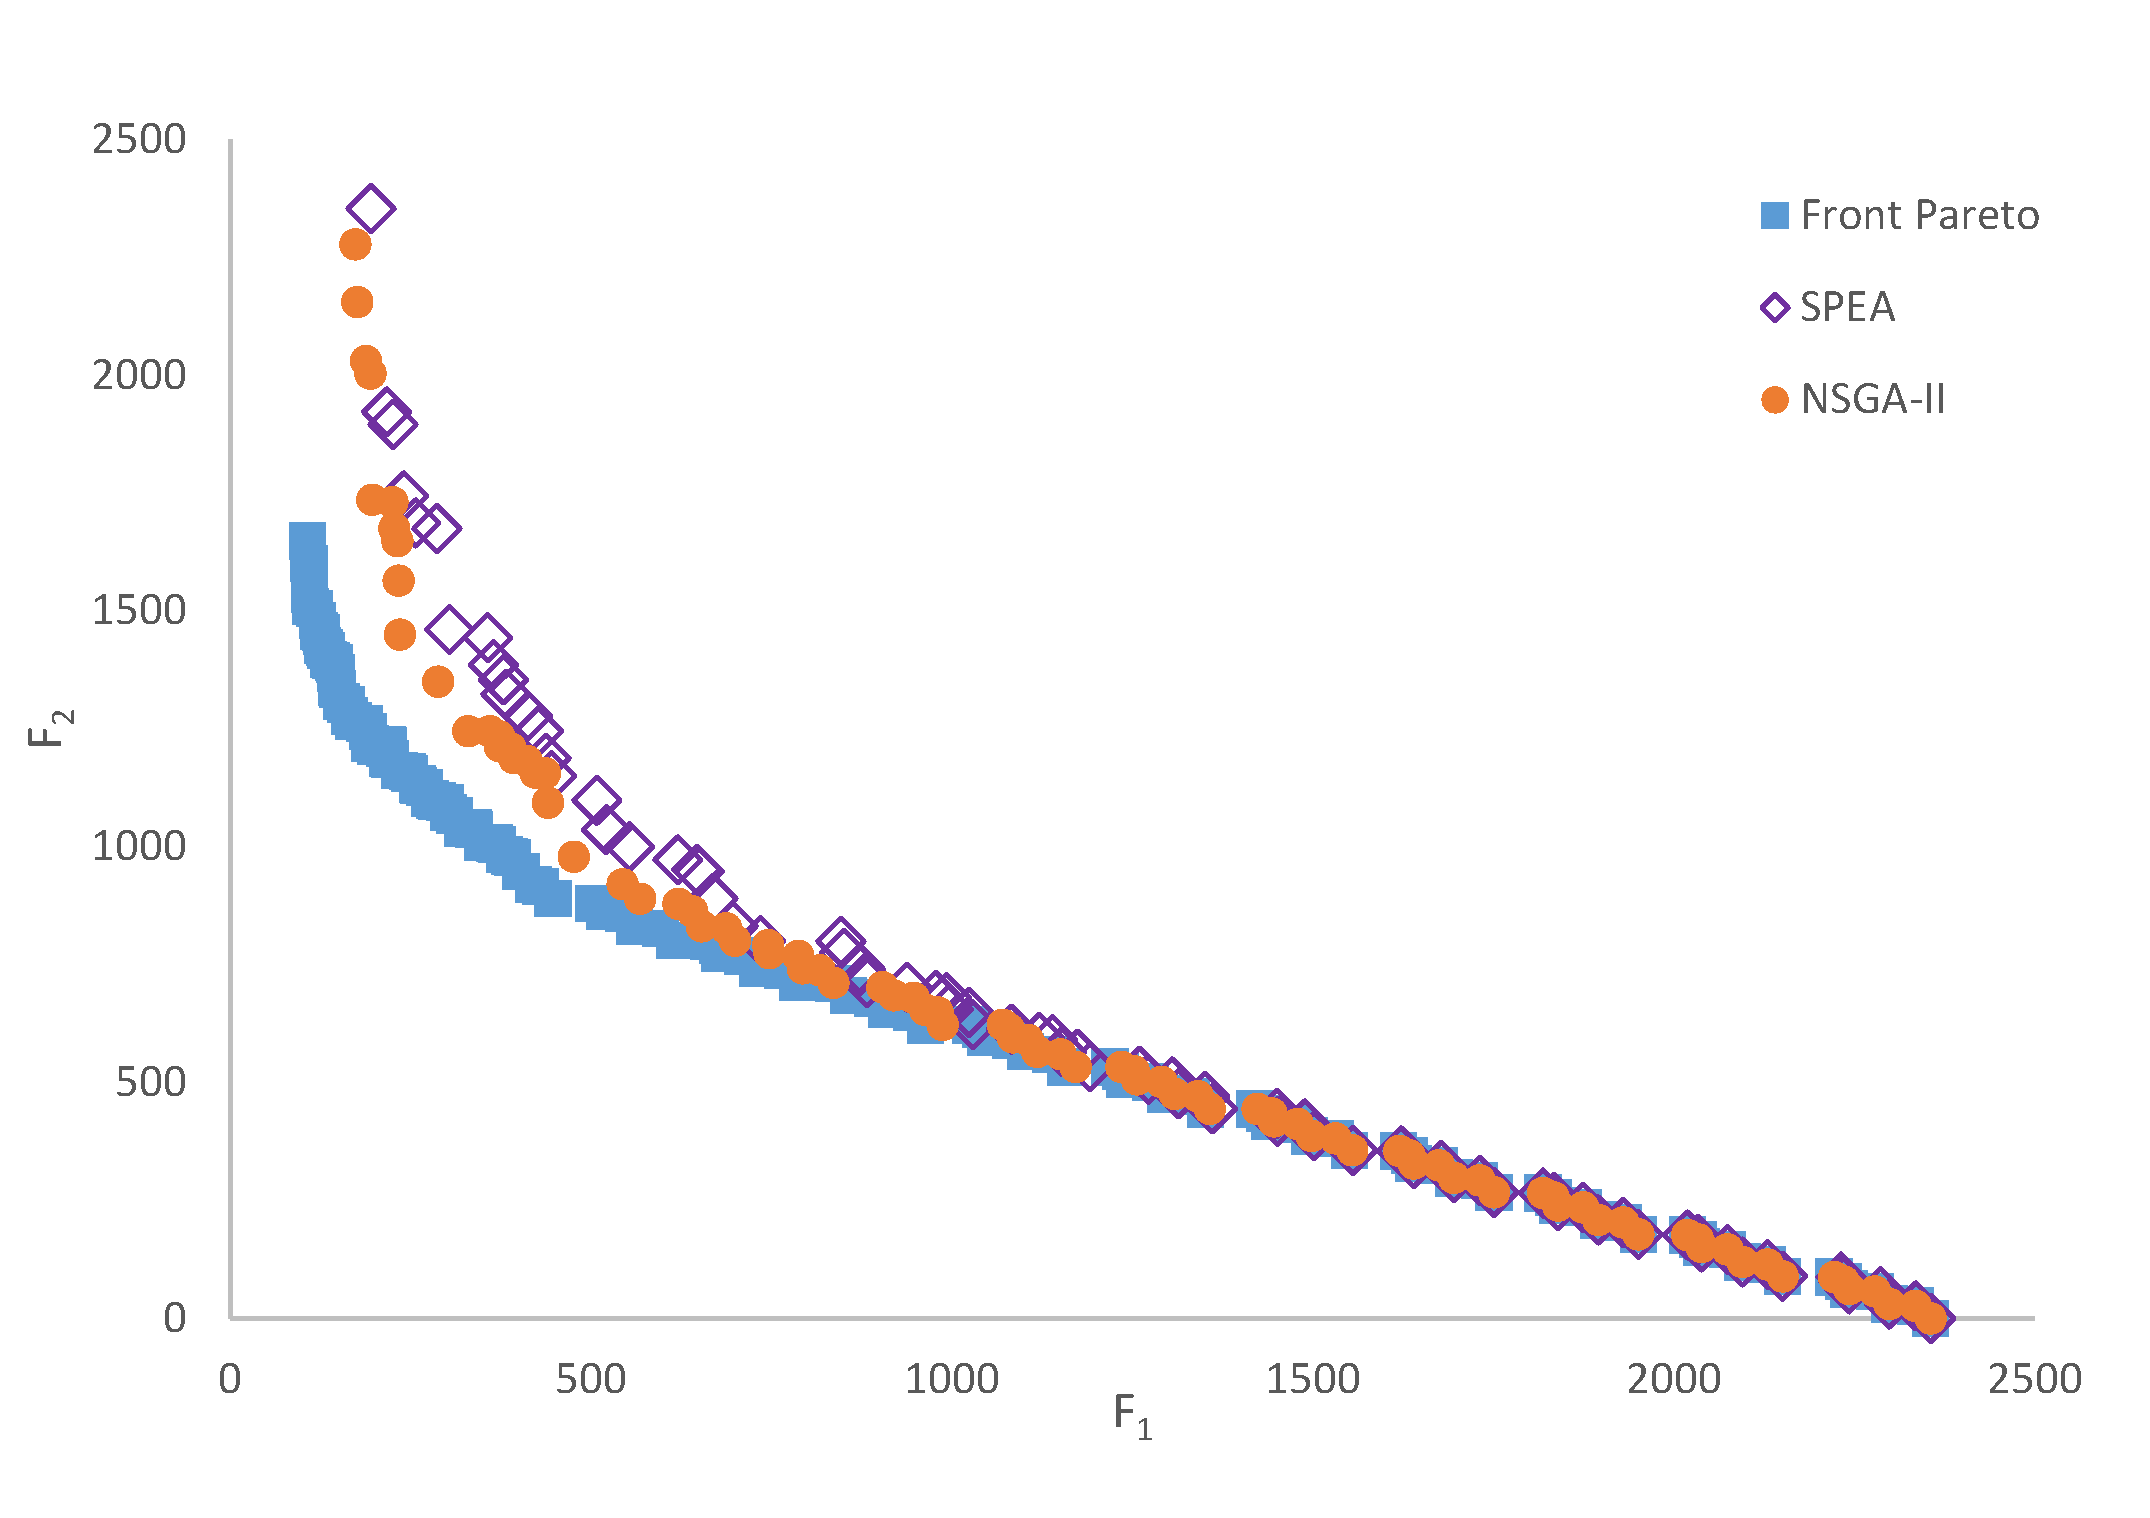
\includegraphics[width=0.5\textwidth]{medium_pareto_100}}
    \hfill
\subfloat[500 generacji\label{fig:medium_pareto_500}]
         {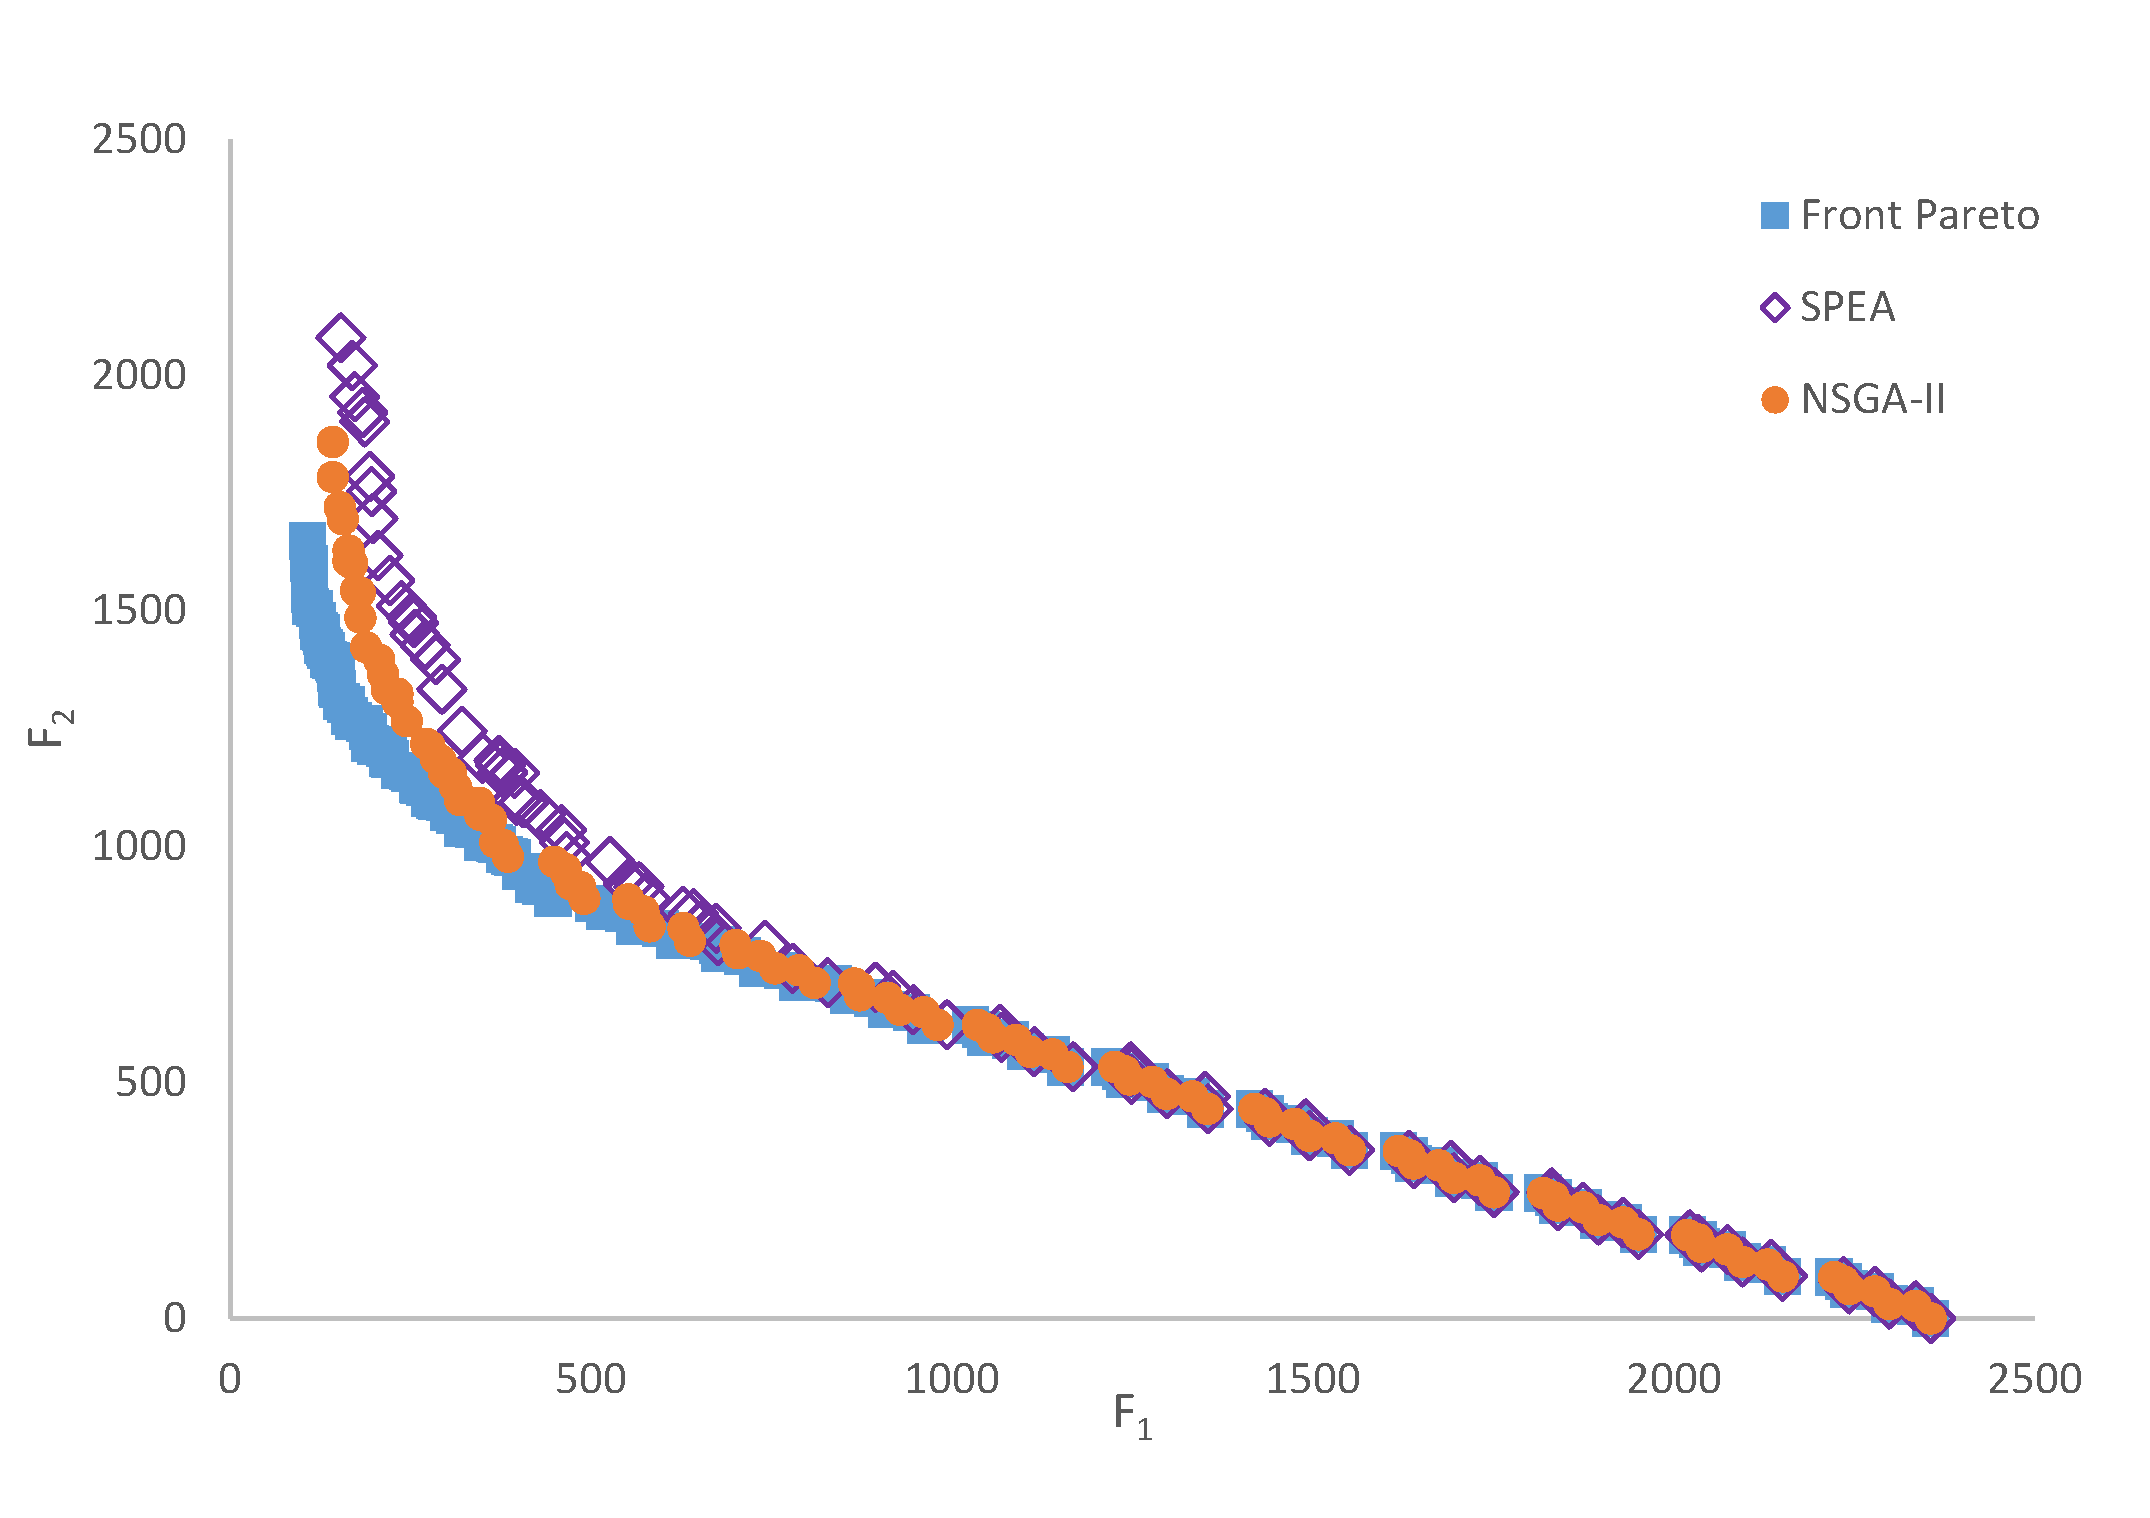
\includegraphics[width=0.5\textwidth]{medium_pareto_500}}
    \hfill
\subfloat[1000 generacji\label{fig:medium_pareto_1000}]
        {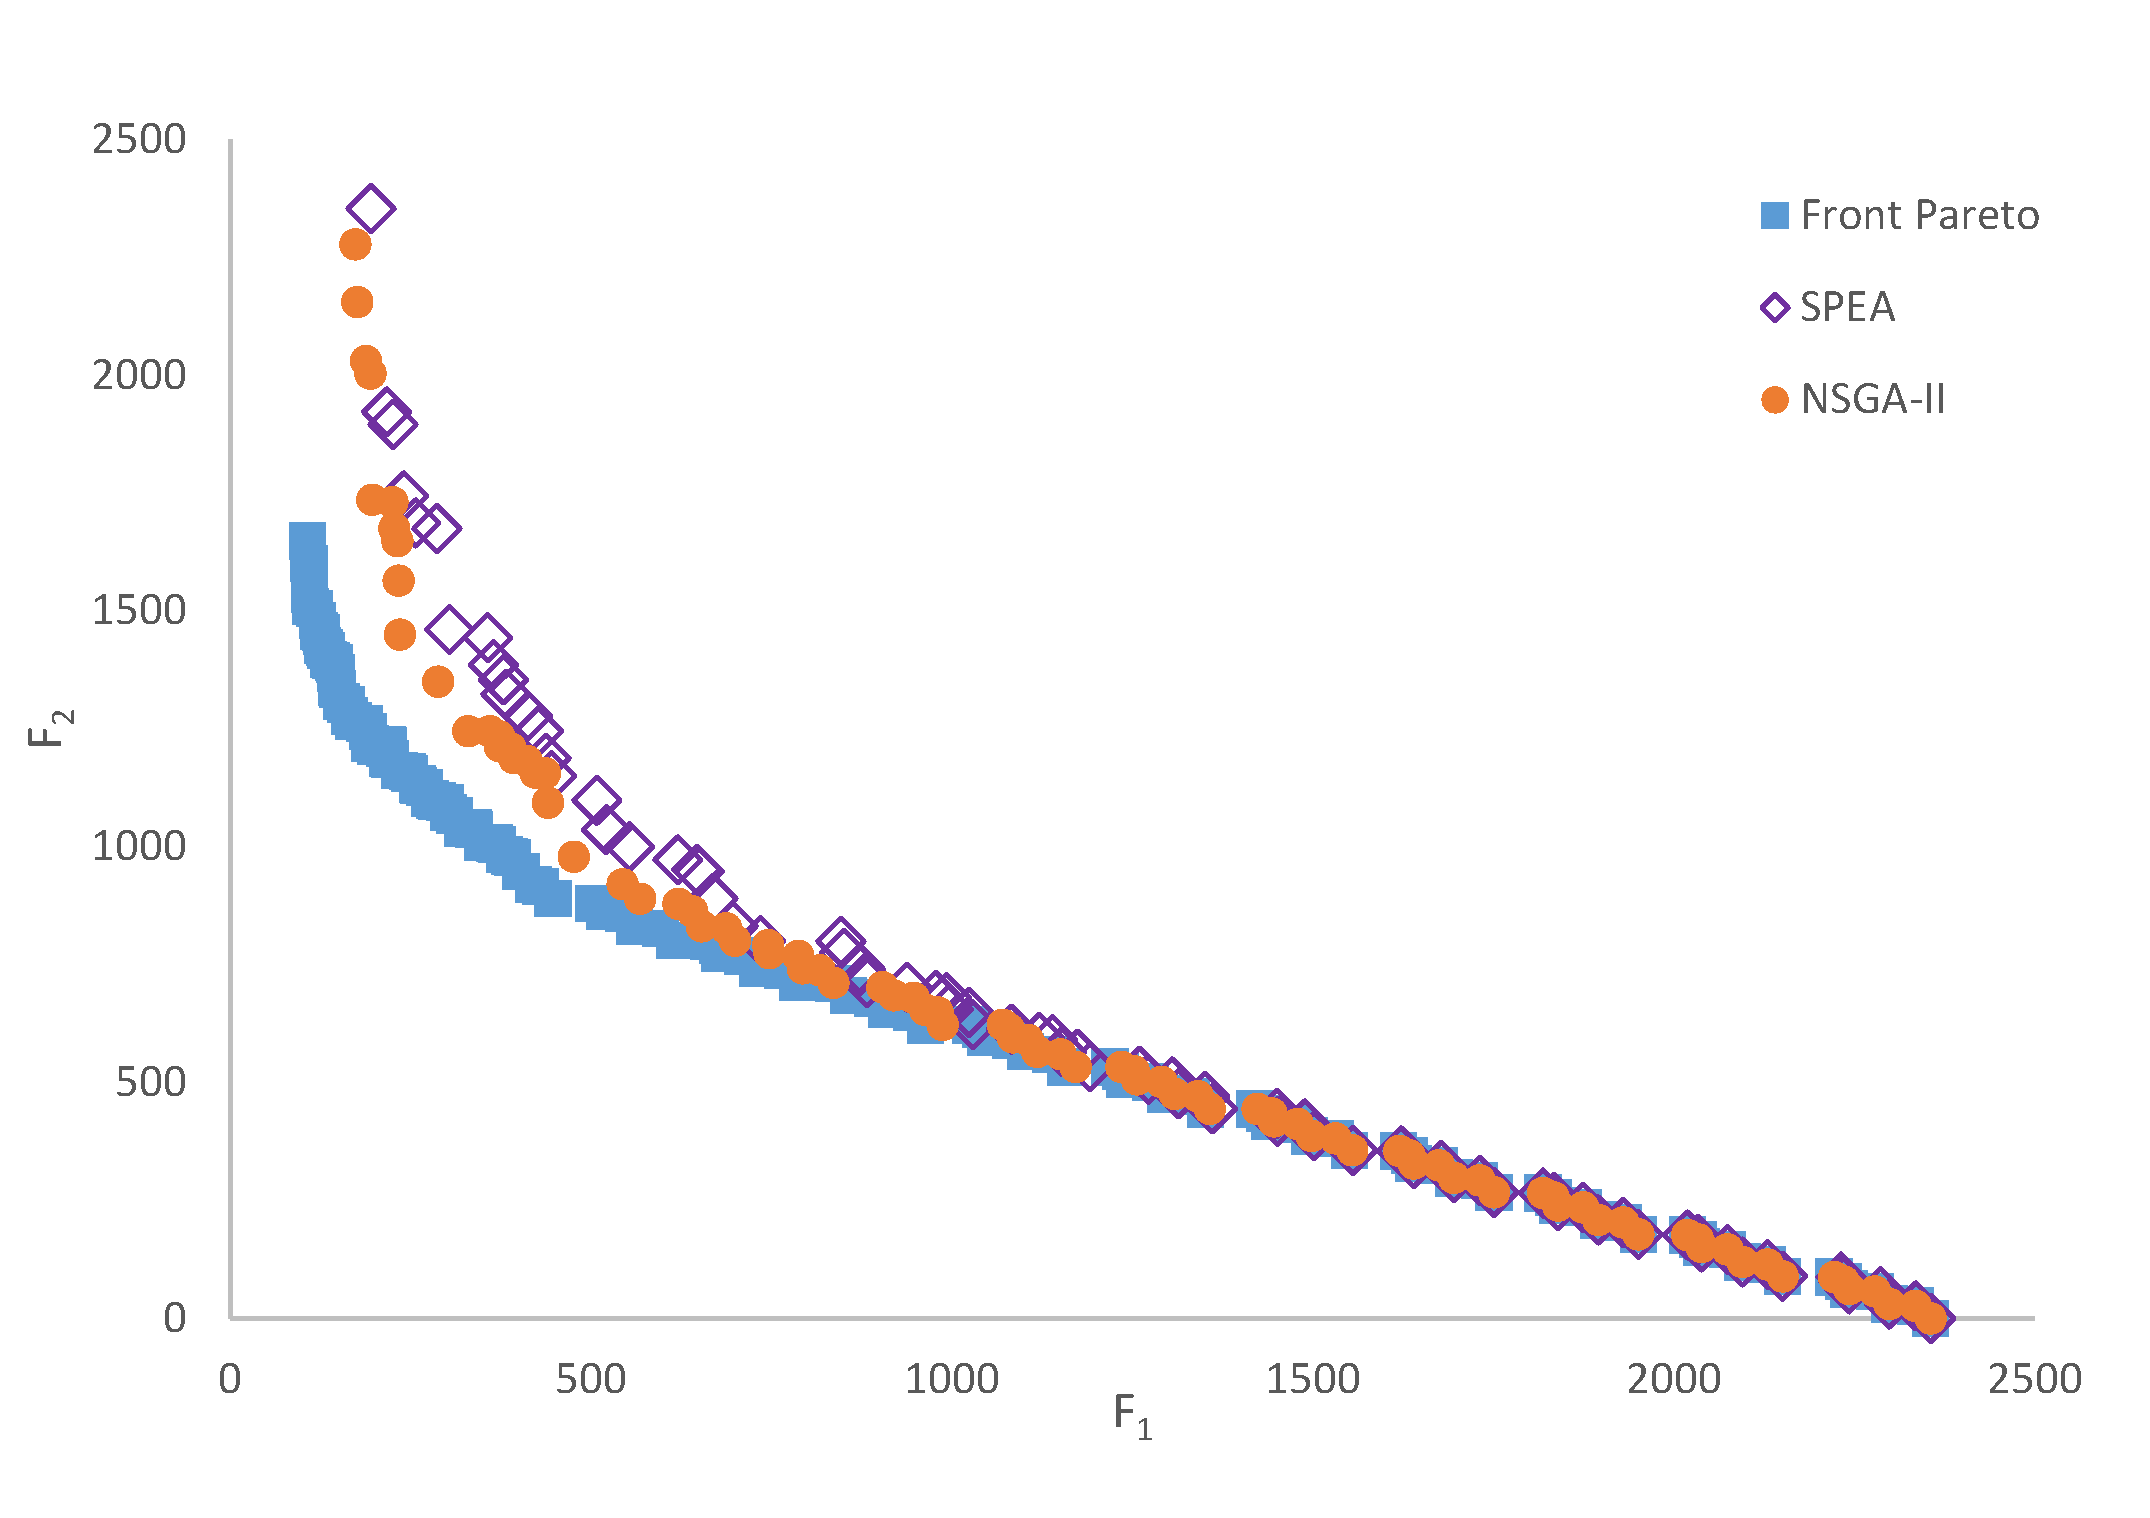
\includegraphics[width=0.5\textwidth]{medium_pareto_1000}}
\subfloat[2000 generacji\label{fig:medium_pareto_2000}]
        {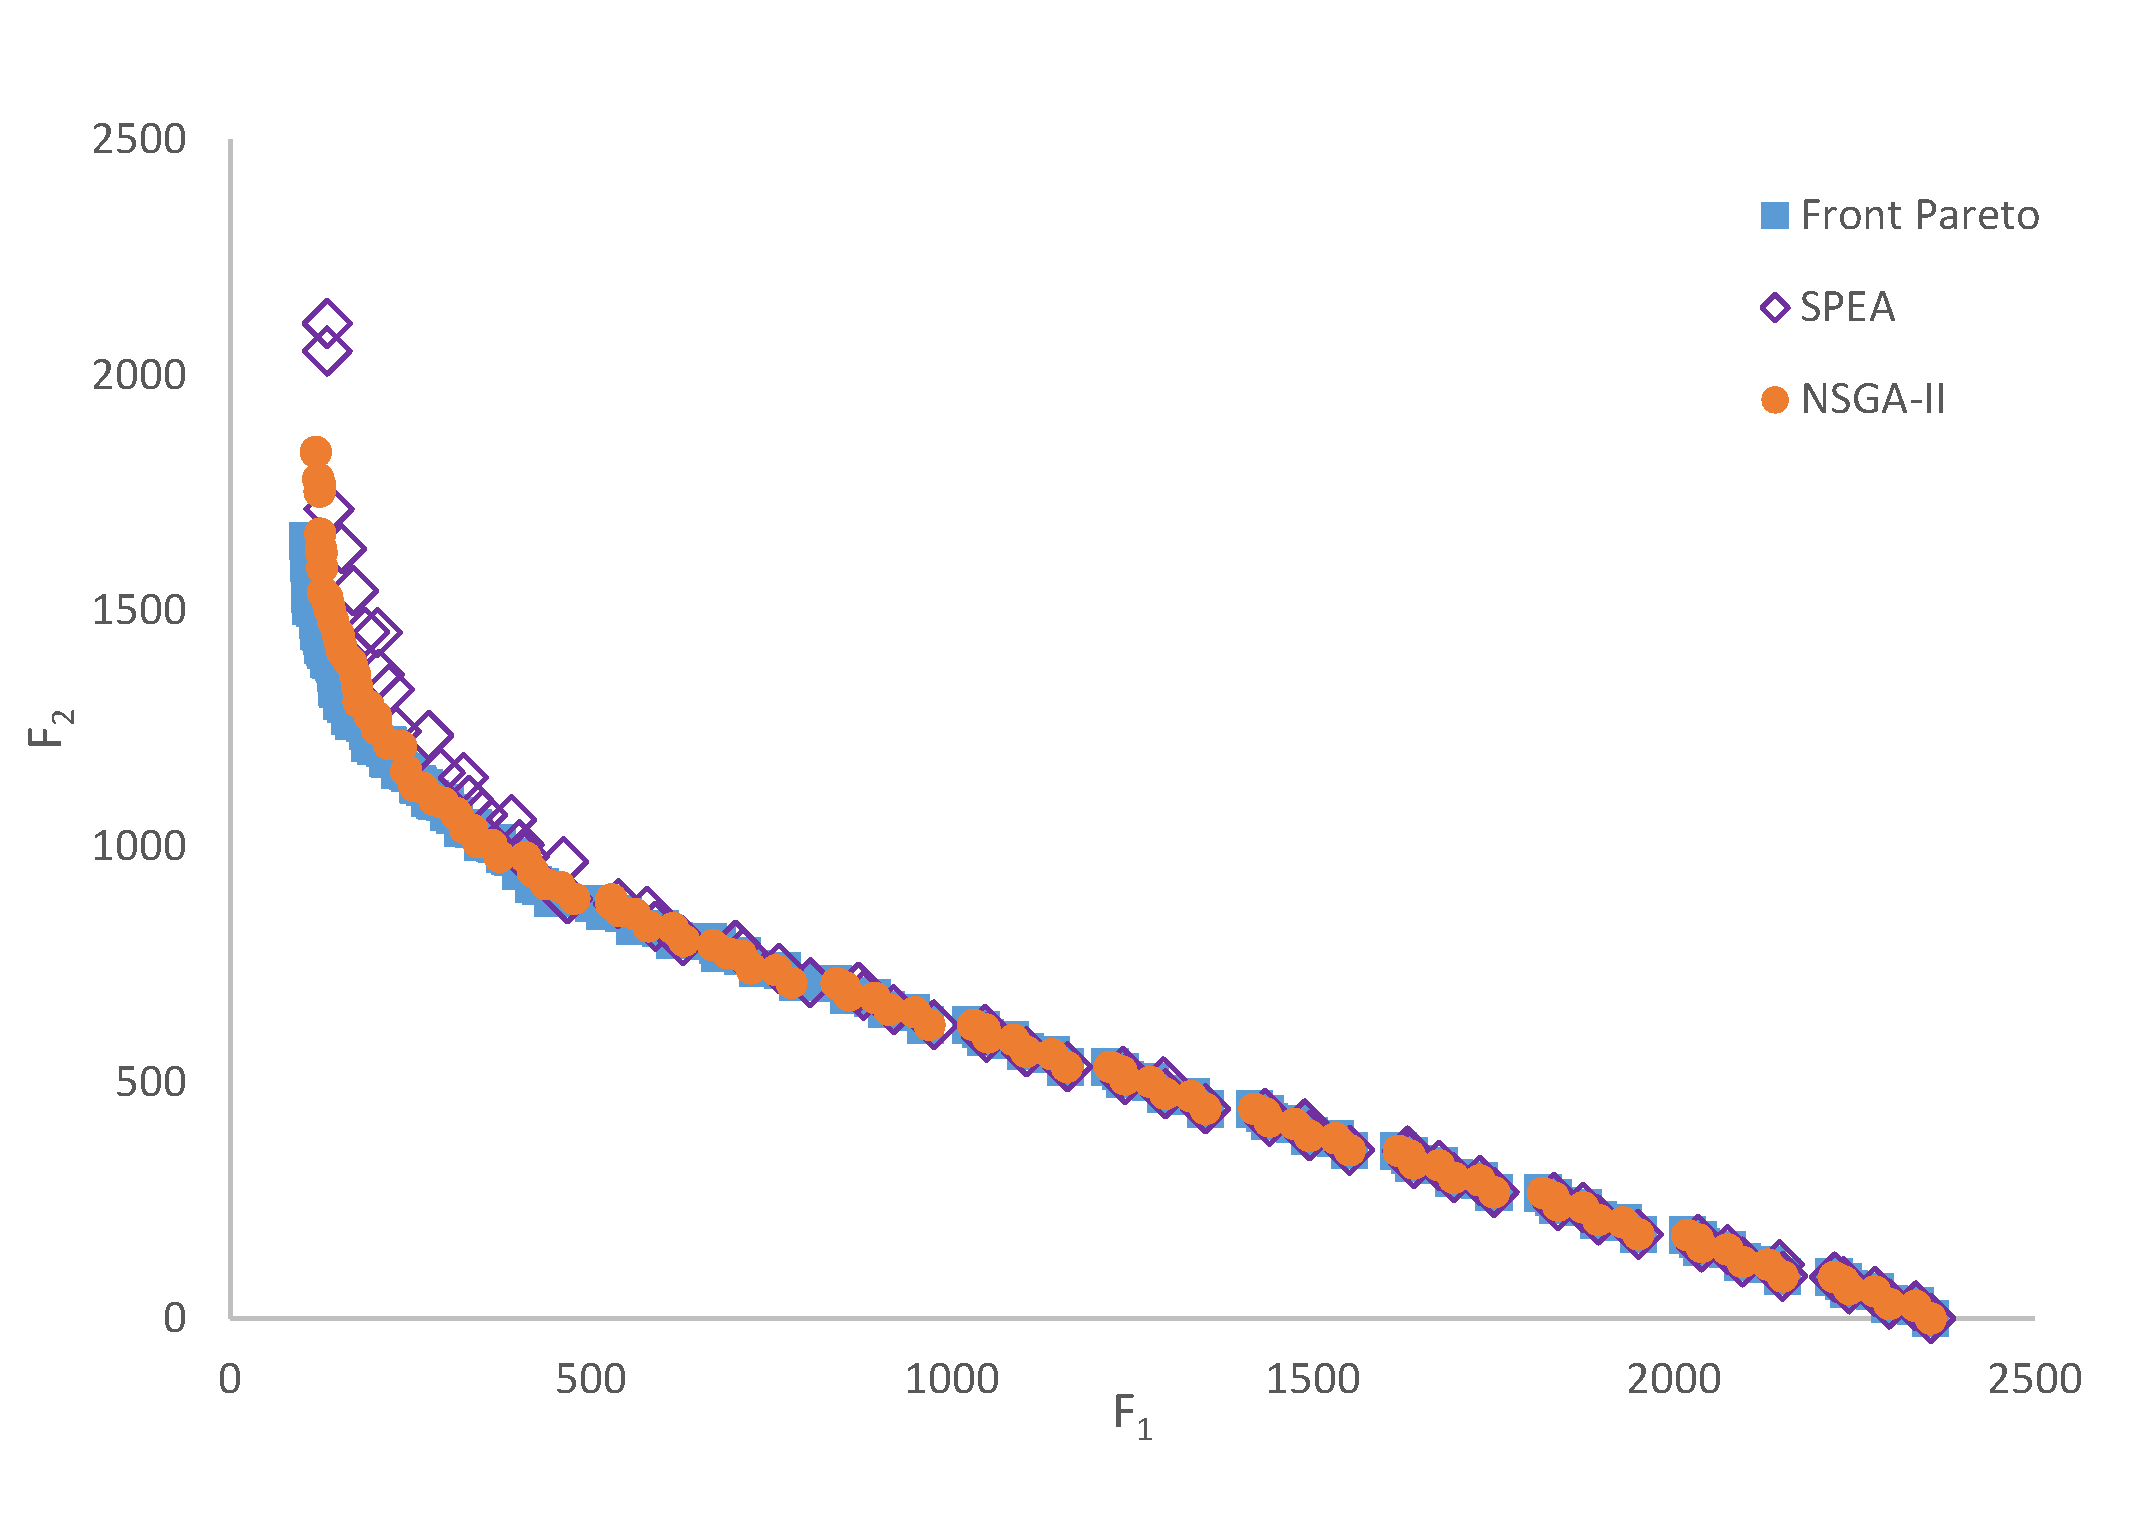
\includegraphics[width=0.5\textwidth]{medium_pareto_2000}}
\caption{Rozwiązania niezdominowane otrzymane dla drugiego przypadku testowego.}
    \label{fig:medium_front}
\end{figure*}
Podobnie jak w poprzednim przypadku algorytmy bardzo szybko znalazły rozwiązania leżące na froncie Pareto oraz charakteryzujące się małą wartością funkcji $F_{2}$ \eqref{fig:medium_front}.

Analizując przedstawione wykresy można łatwo zauważyć, że algorytm NSGA-II w każdym z przedstawionych pokoleń wygenerował rozwiązania lepsze od tych znalezionych przez SPEA.

Jest to najlepiej widoczne na wykresie prezentującym wyniku po 500. pokoleniu. Dla dużych wartości funkcji $F_{2}$, gdzie front Pareto jeszcze nie został osiągnięty, żadne rozwiązanie znalezione przez NSGA-II nie jest zdominowane przez jakiekolwiek rozwiązanie wygenerowane przez SPEA. Taka sytuacja utrzymała się, aż do końca symulacji.
Powyżej opisane obserwacje znajdują swoje odzwierciedlenie w wartościach metryk \eqref{fig:medium_metrics}. NSGA-II przez cały czas trwania symulacji znajdował rozwiązania charakteryzujące się lepszą wartością metryk $GD$ oraz $SP$. Co ciekawe SPEA wygenerował dłuższy front rozwiązań, co jednak nie przekłada się na całościową ocenę algorytmu.
\begin{figure*}\centering
\subfloat[Współczynnik błędu (ER)\label{fig:er_medium}]
        {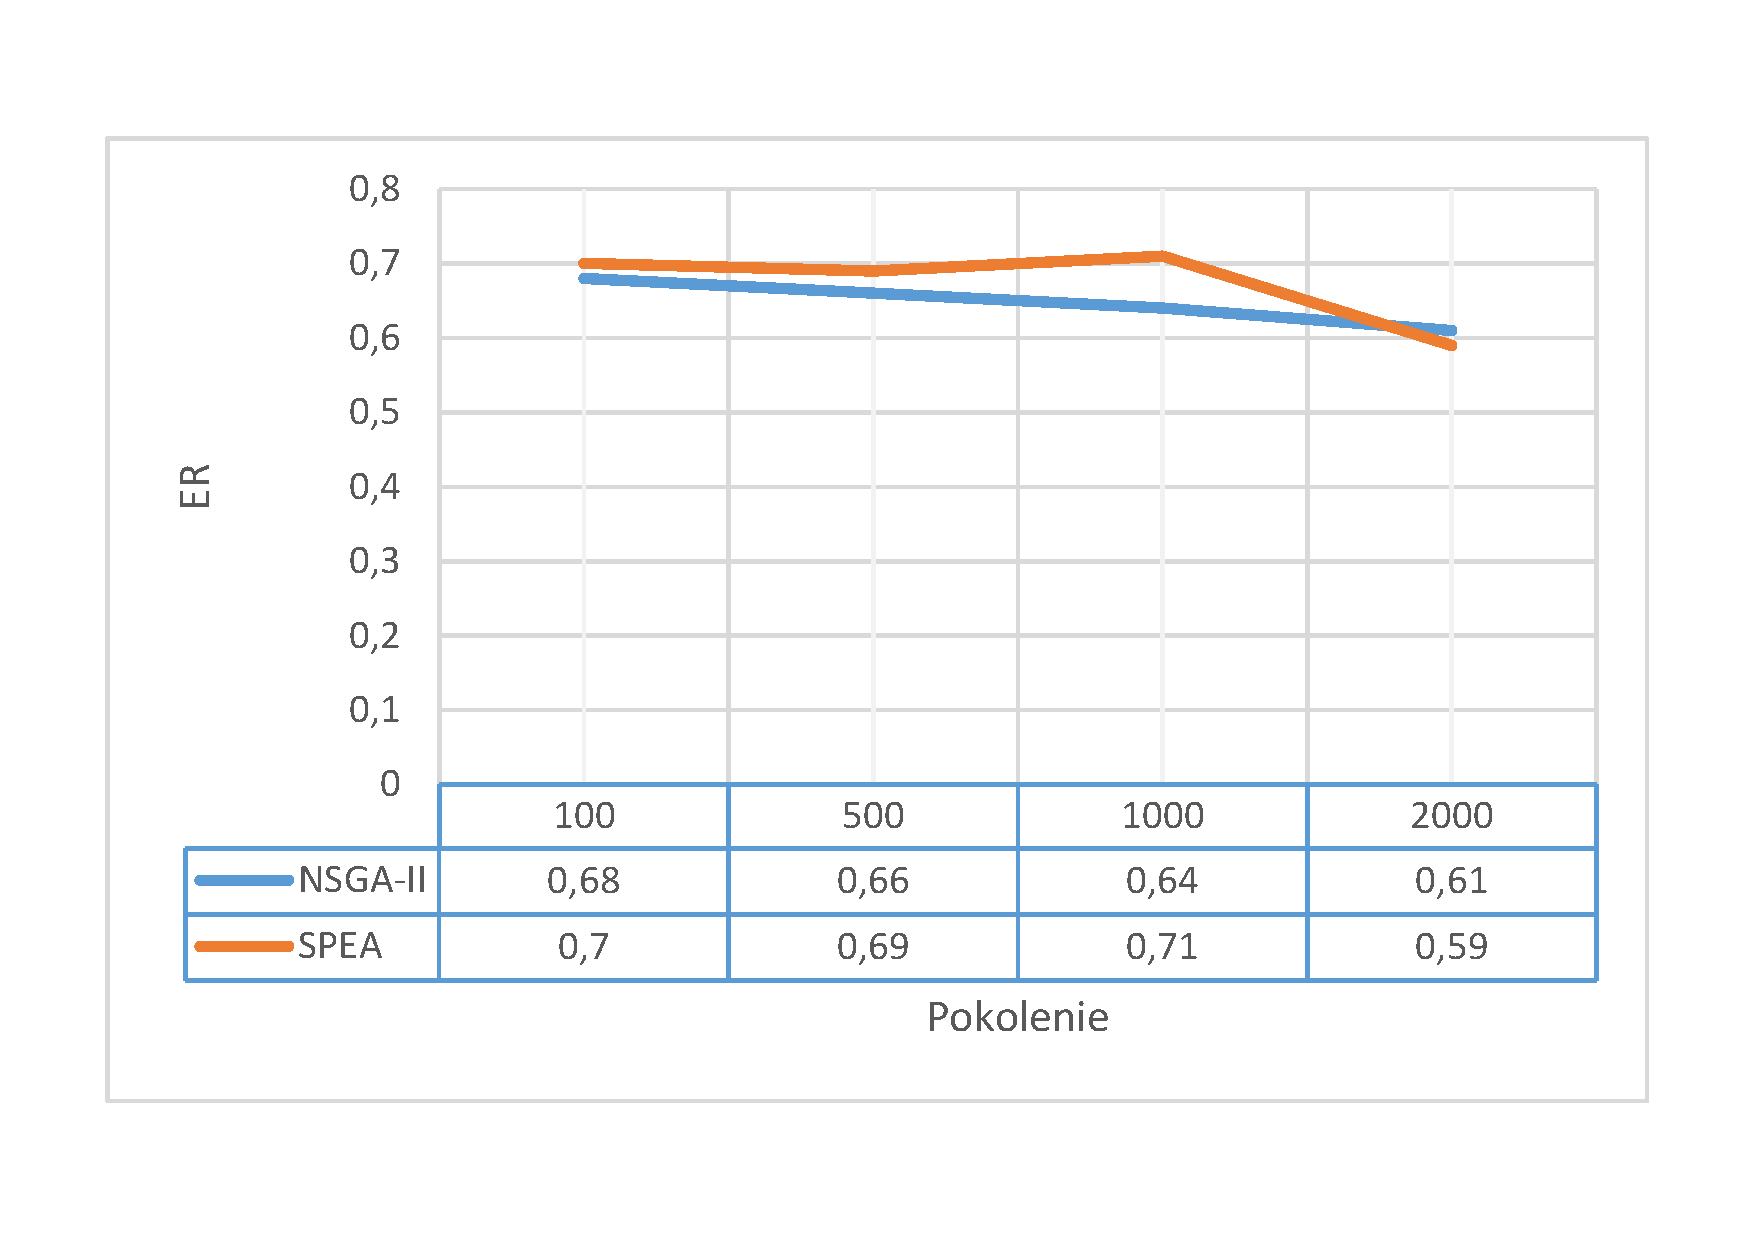
\includegraphics[width=0.5\textwidth]{er_medium}}
    \hfill
\subfloat[Długość frontu (FE)\label{fig:fe_medium}]
         {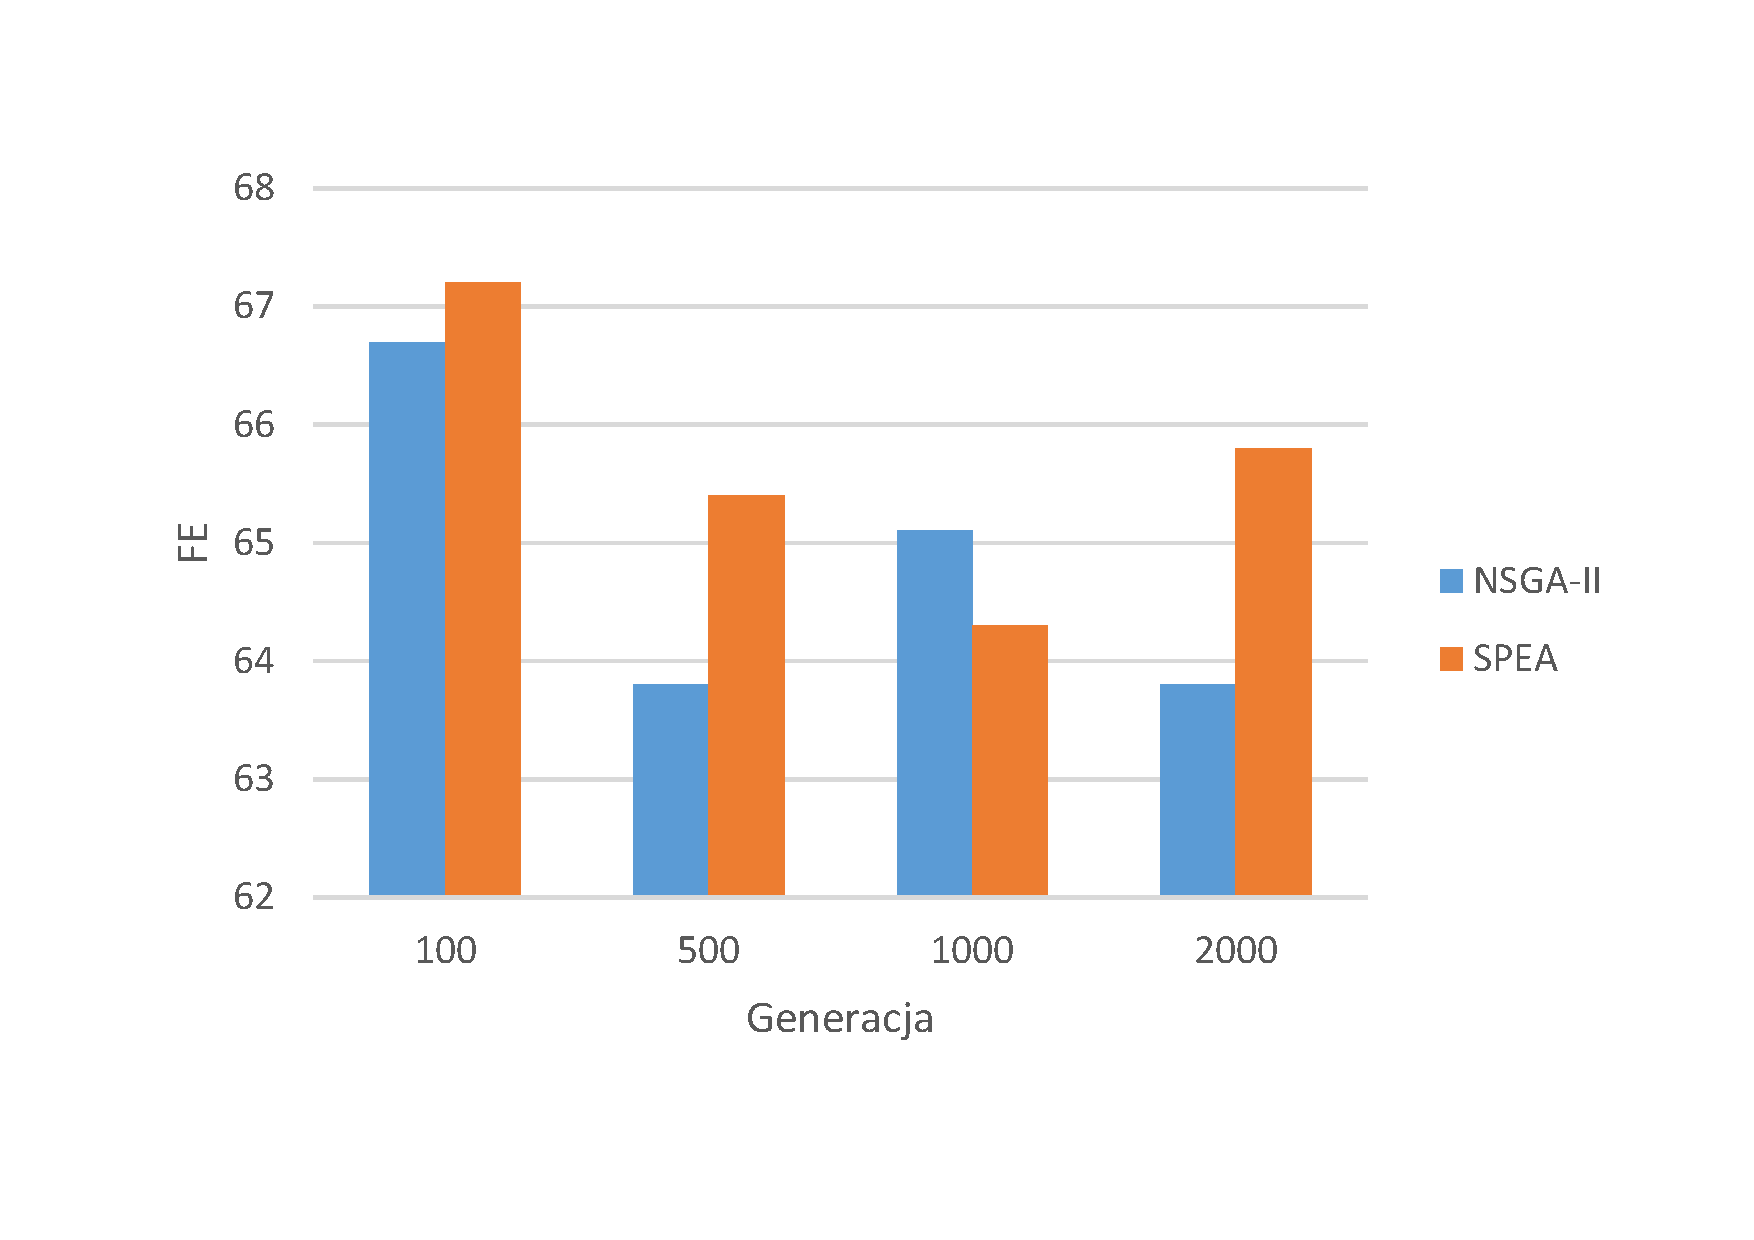
\includegraphics[width=0.5\textwidth]{fe_medium}}

\subfloat[Jakość ogólna (GD)\label{fig:gd_medium}]
         {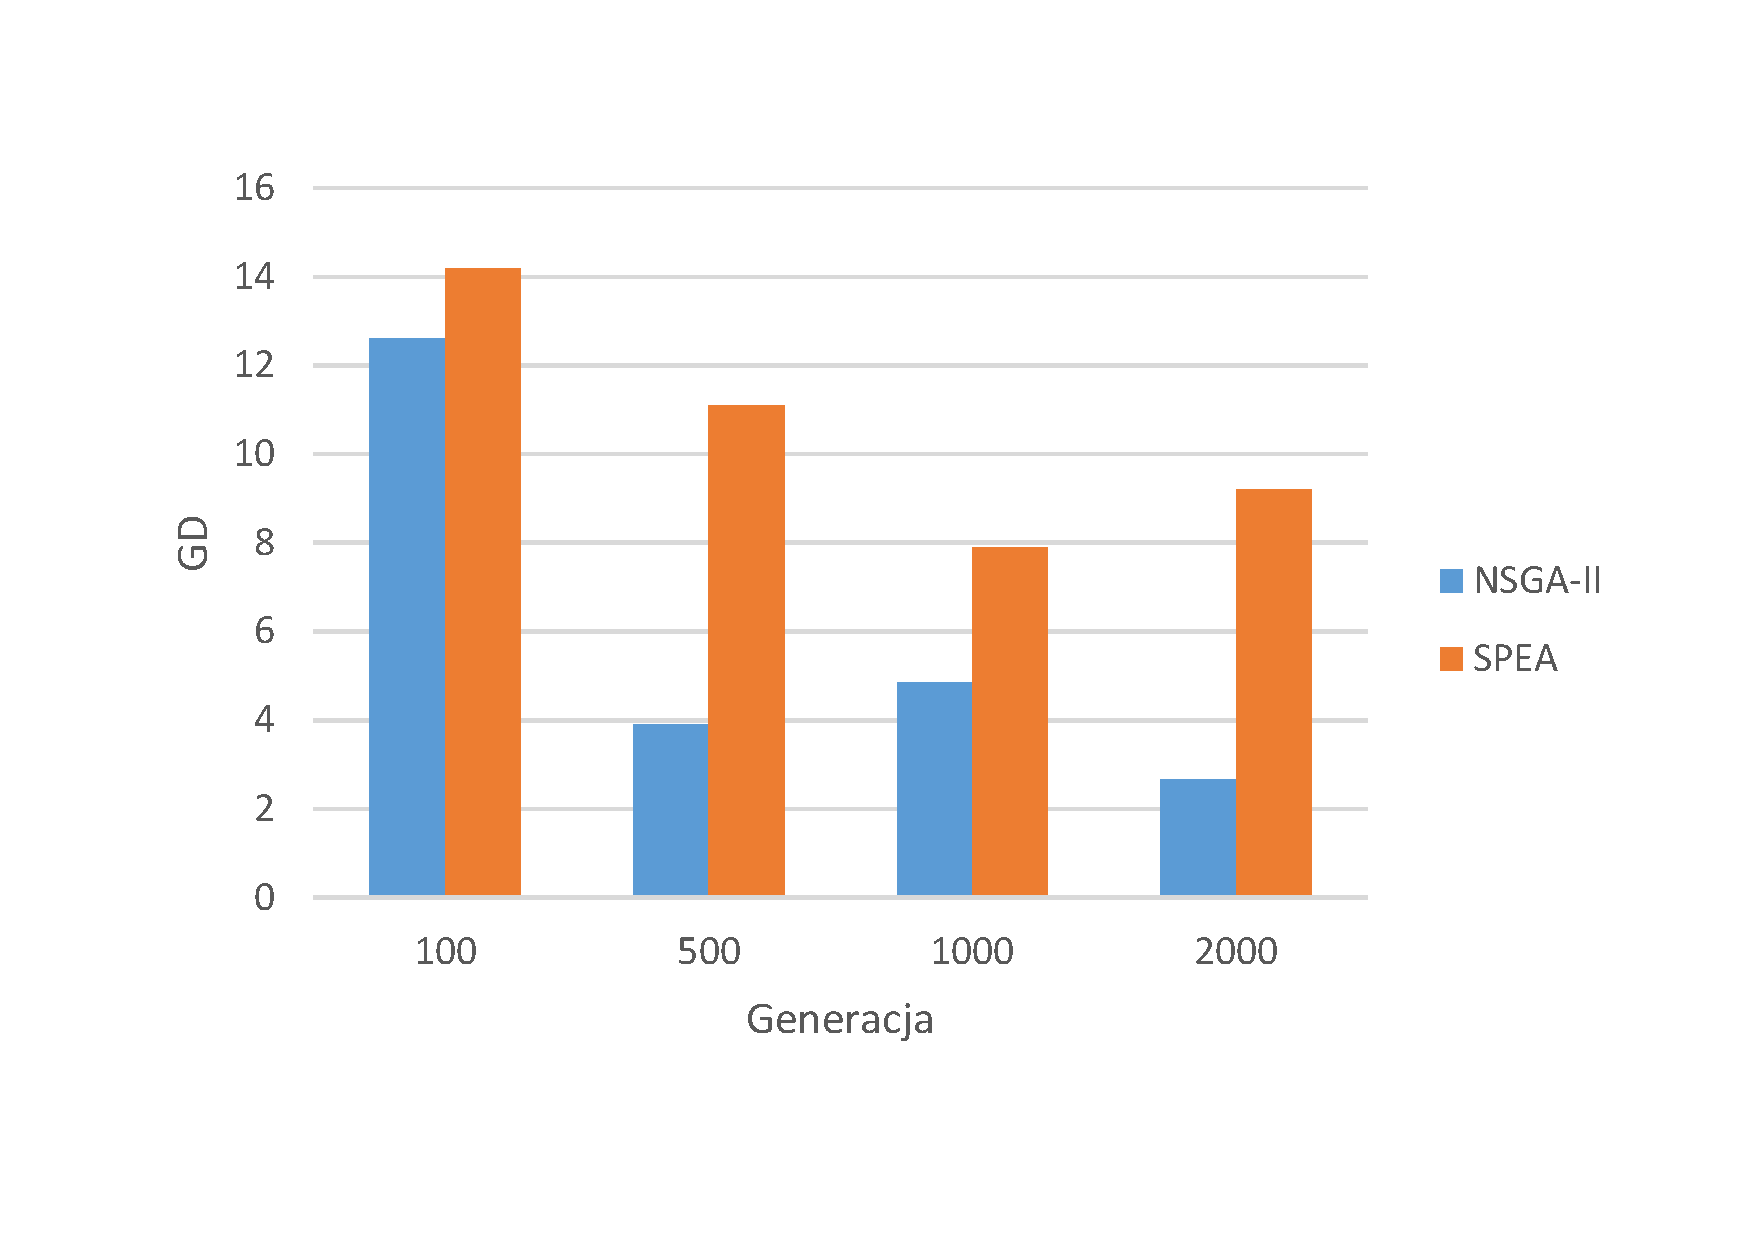
\includegraphics[width=0.5\textwidth]{gd_medium}}
    \hfill
\subfloat[Równomierność rozkładu (SP)\label{fig:sp_medium}]
        {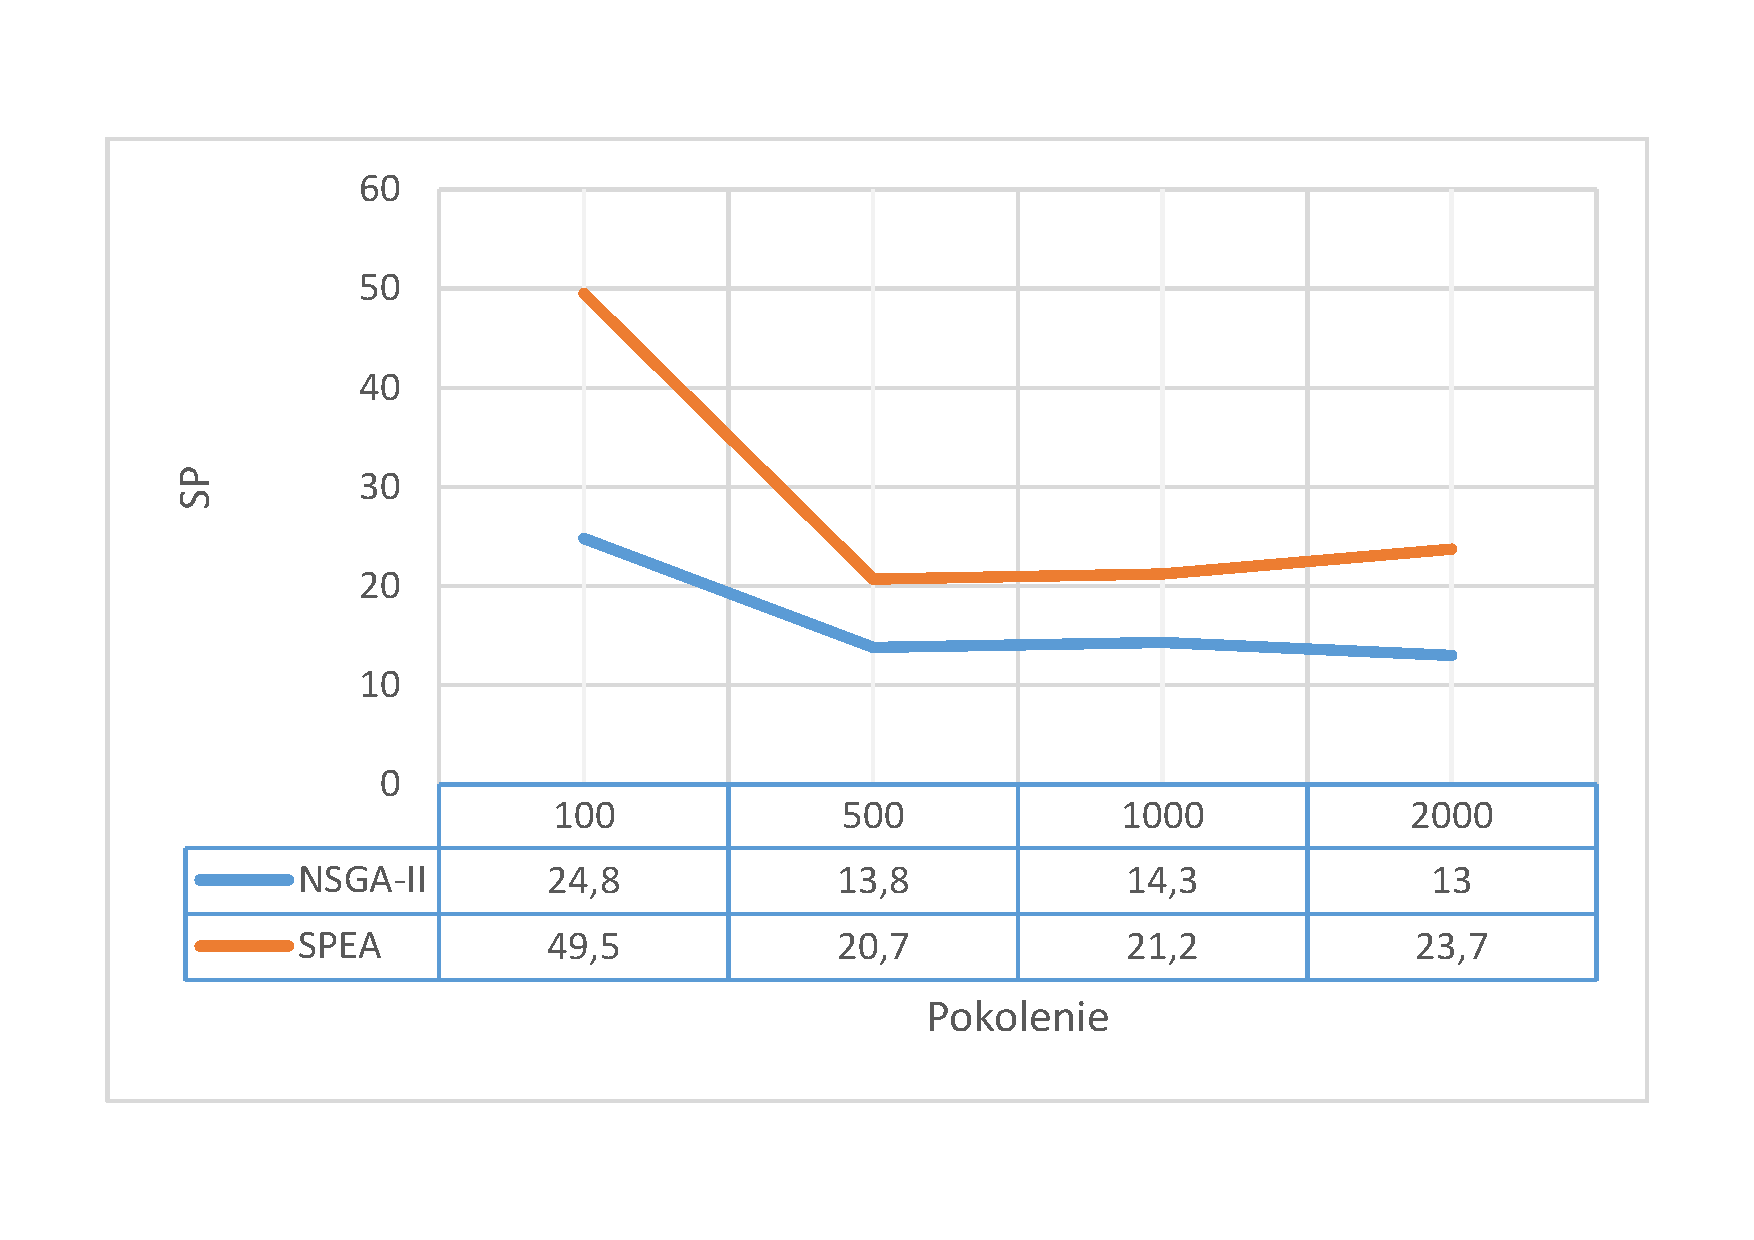
\includegraphics[width=0.5\textwidth]{sp_medium}}
\caption{Wartość metryk charakteryzujących wyniki symulacji dla drugiego przypadku testowego.}
    \label{fig:medium_metrics}
\end{figure*}

Podsumowując, z drugim przypadkiem testowym zdecydowanie lepiej poradził sobie algorytm NSGA-II.\newpage
\subsubsection{Trzeci przypadek testowy - obszar duży}
Dla trzeciego przypadku testowego \eqref{fig:big_area} algorytmy uruchomione zostały z ograniczeniem 5000 pokoleń. Ponadto, podobnie jak w poprzednich przypadkach, przeanalizowano dane wygenerowane również przy 100, 1000 oraz 2000 pokoleniu.
\begin{figure}[H]
	\makebox[\textwidth]{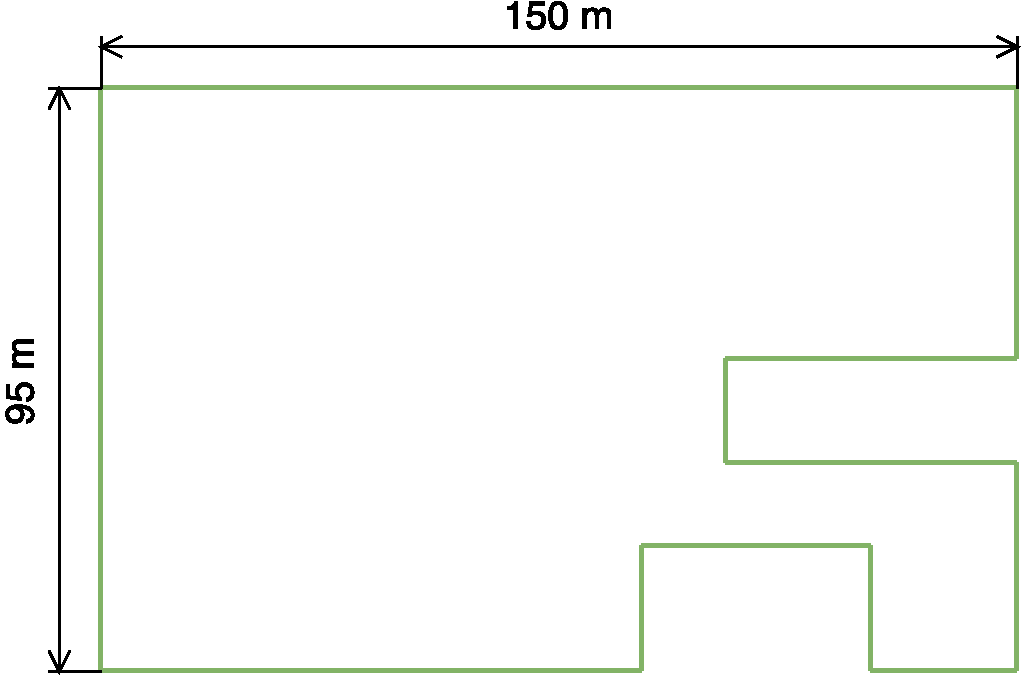
\includegraphics[ clip, scale=0.4]{big_area}}
	\centering
	\caption{Trzeci przypadek testowy - obszar duży.}
	\label{fig:big_area}
\end{figure}
\begin{figure*}\centering
\subfloat[100 generacji\label{fig:big_pareto_100}]
        {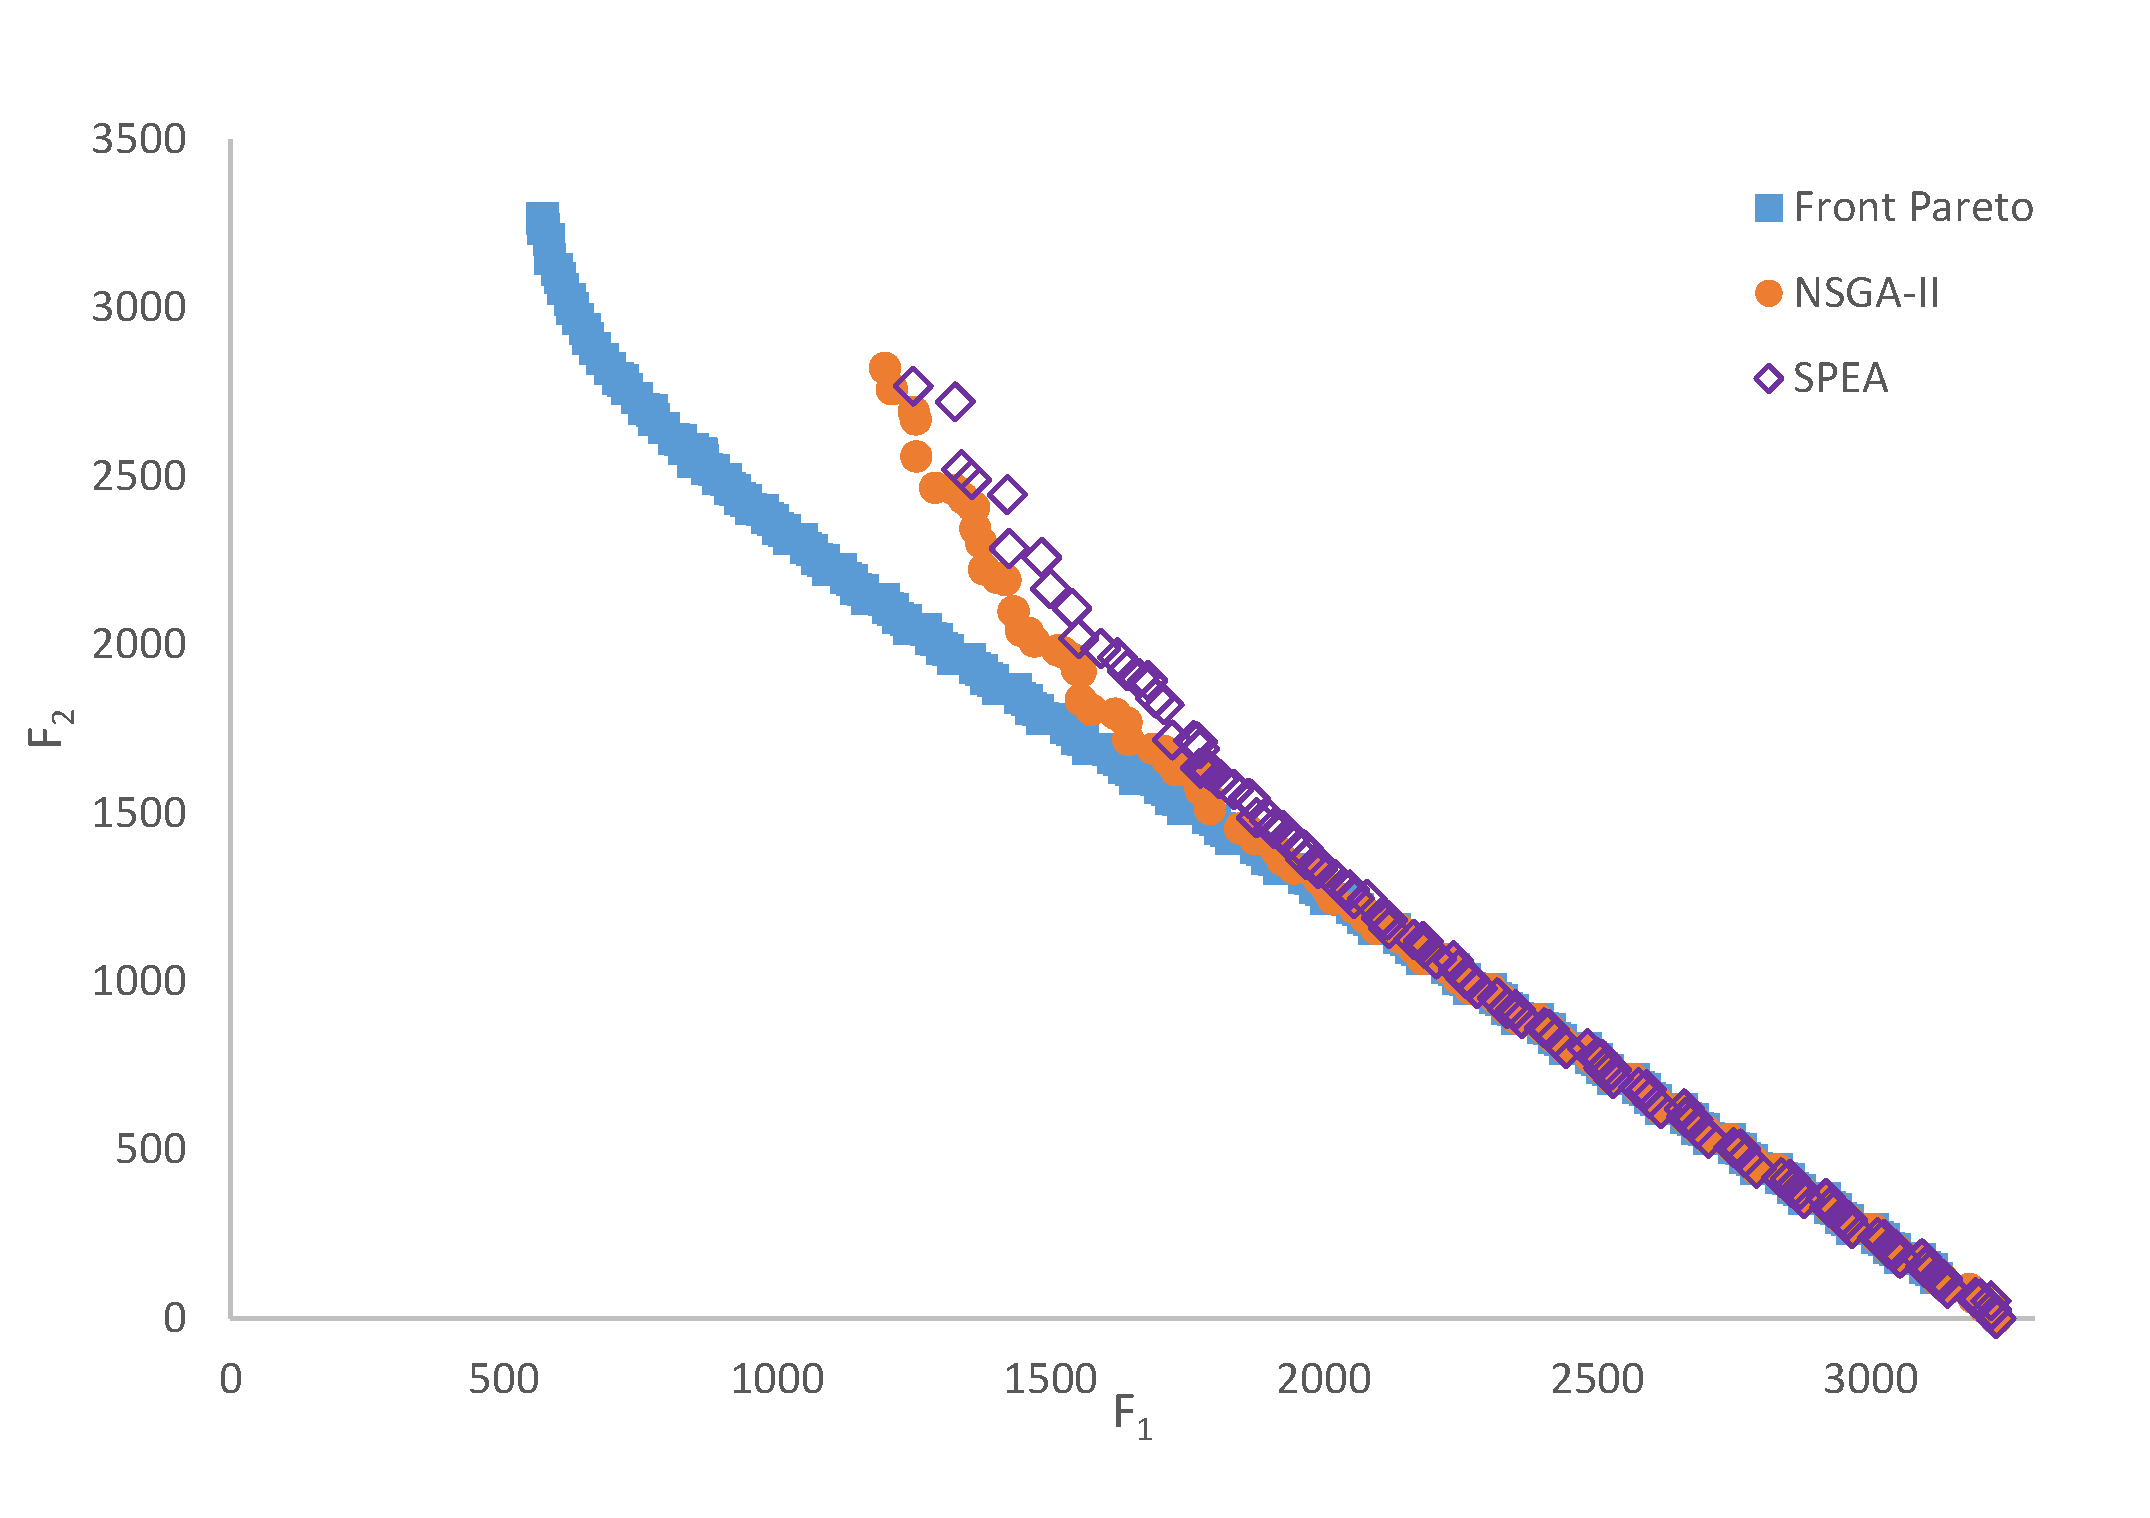
\includegraphics[width=0.5\textwidth]{big_pareto_100}}
    \hfill
\subfloat[1000 generacji\label{fig:big_pareto_1000}]
         {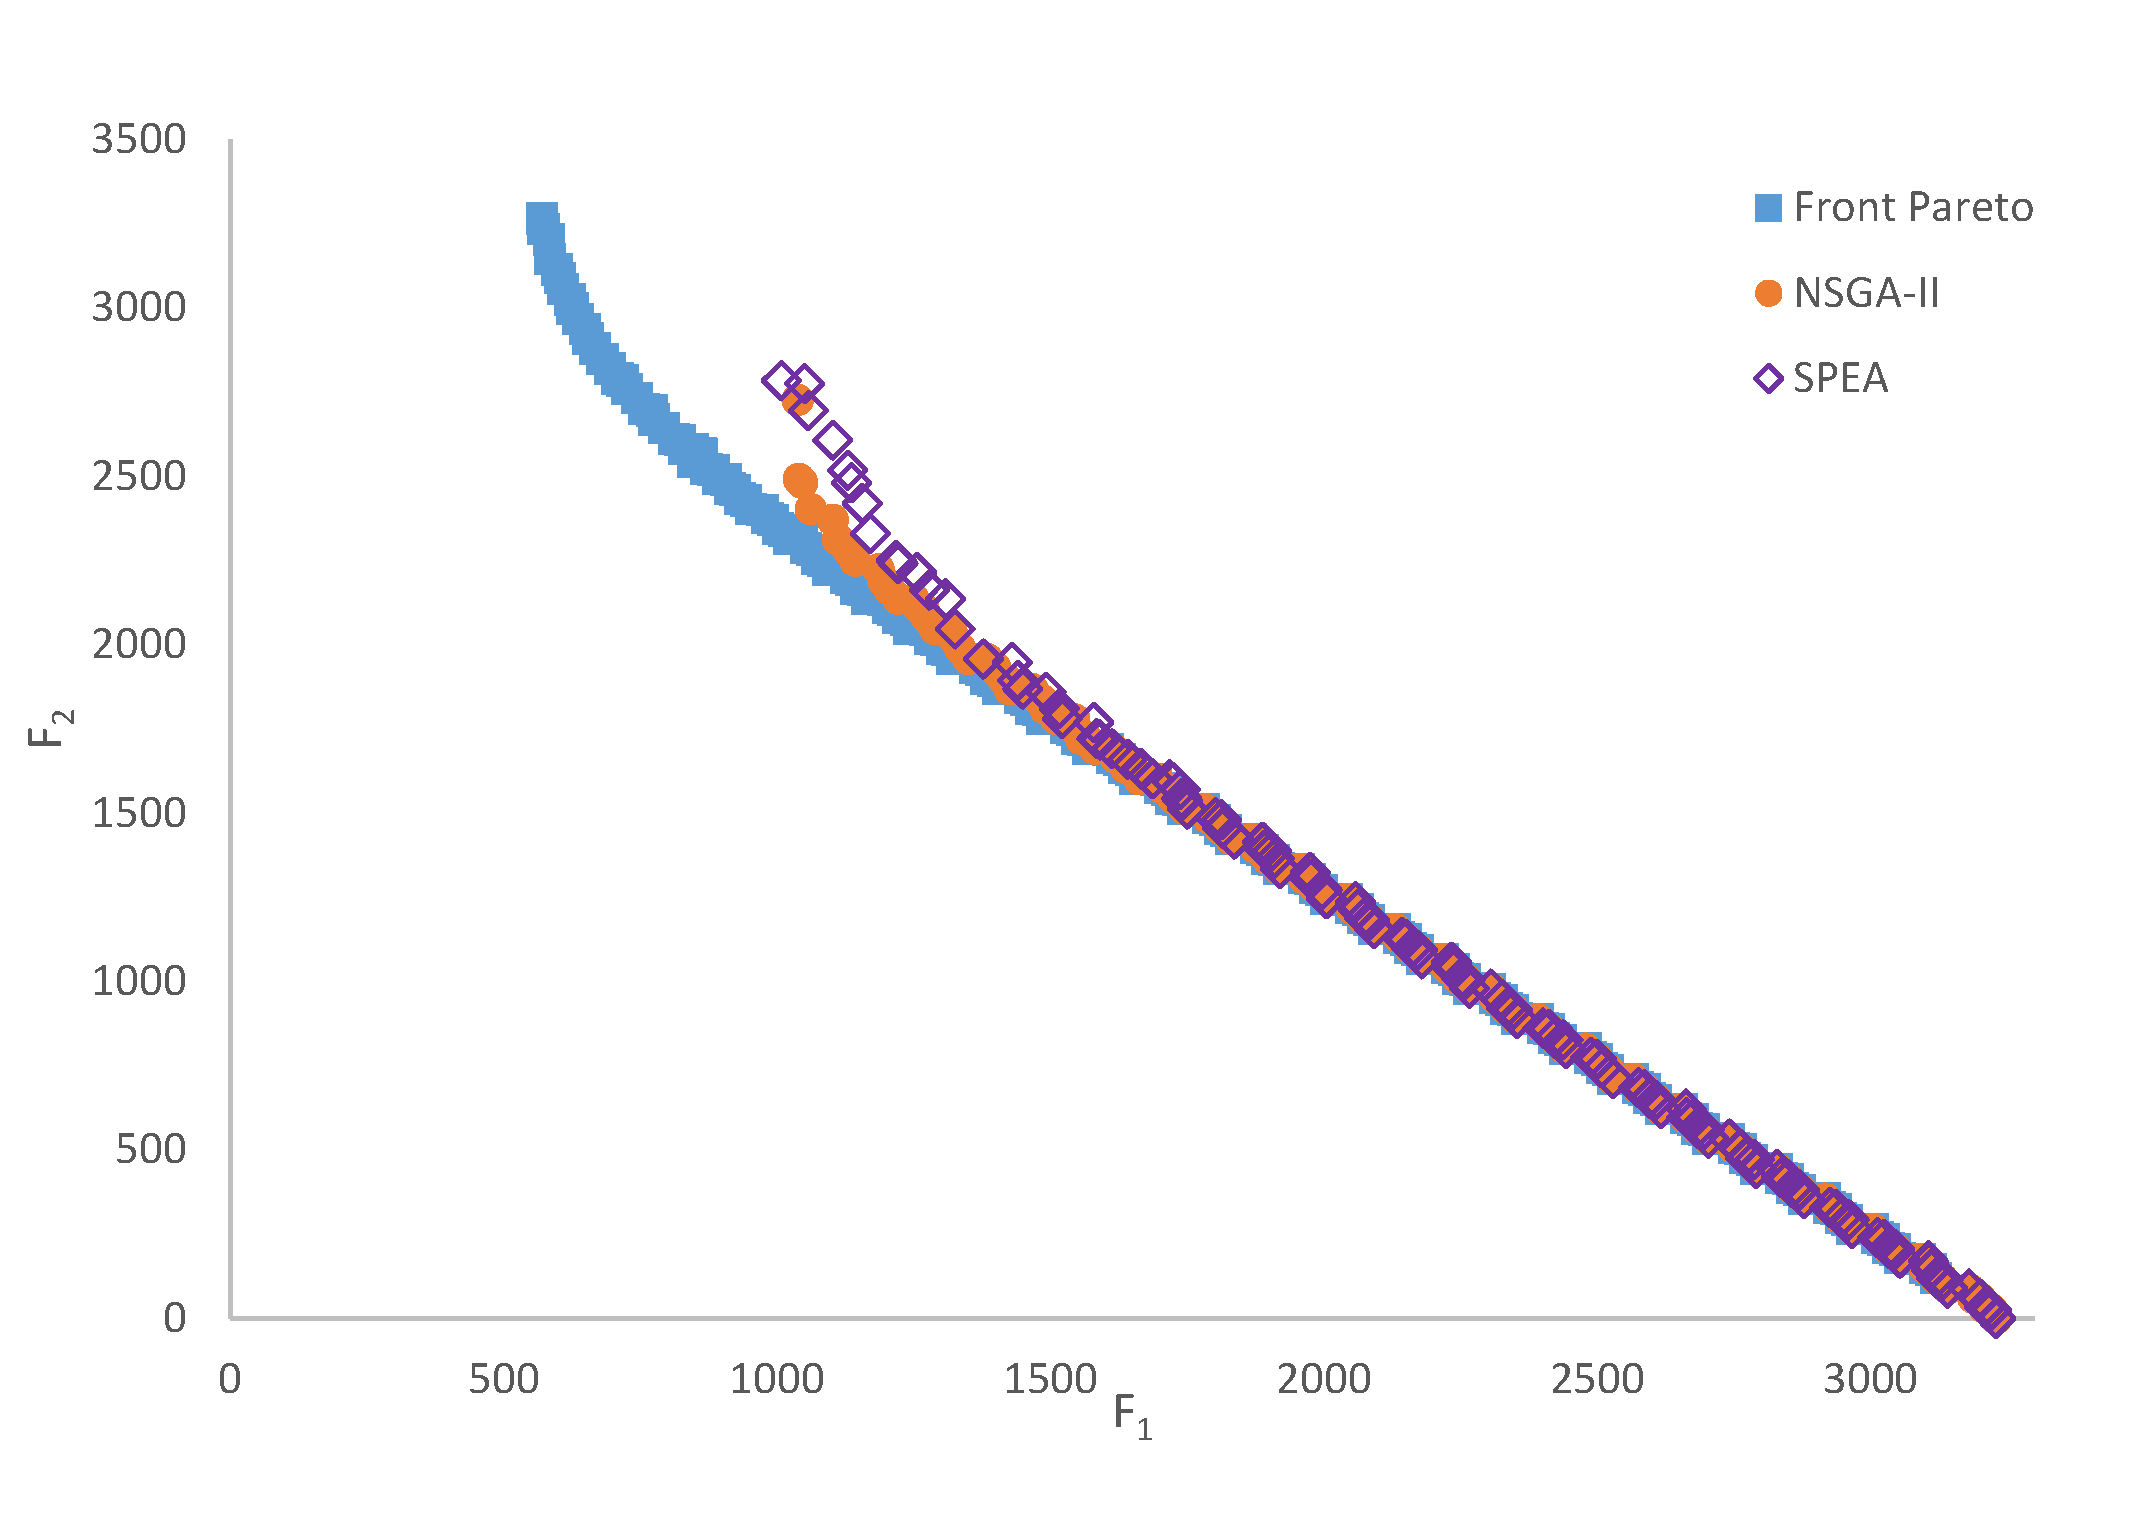
\includegraphics[width=0.5\textwidth]{big_pareto_1000}}
    \hfill
\subfloat[2000 generacji\label{fig:big_pareto_2000}]
        {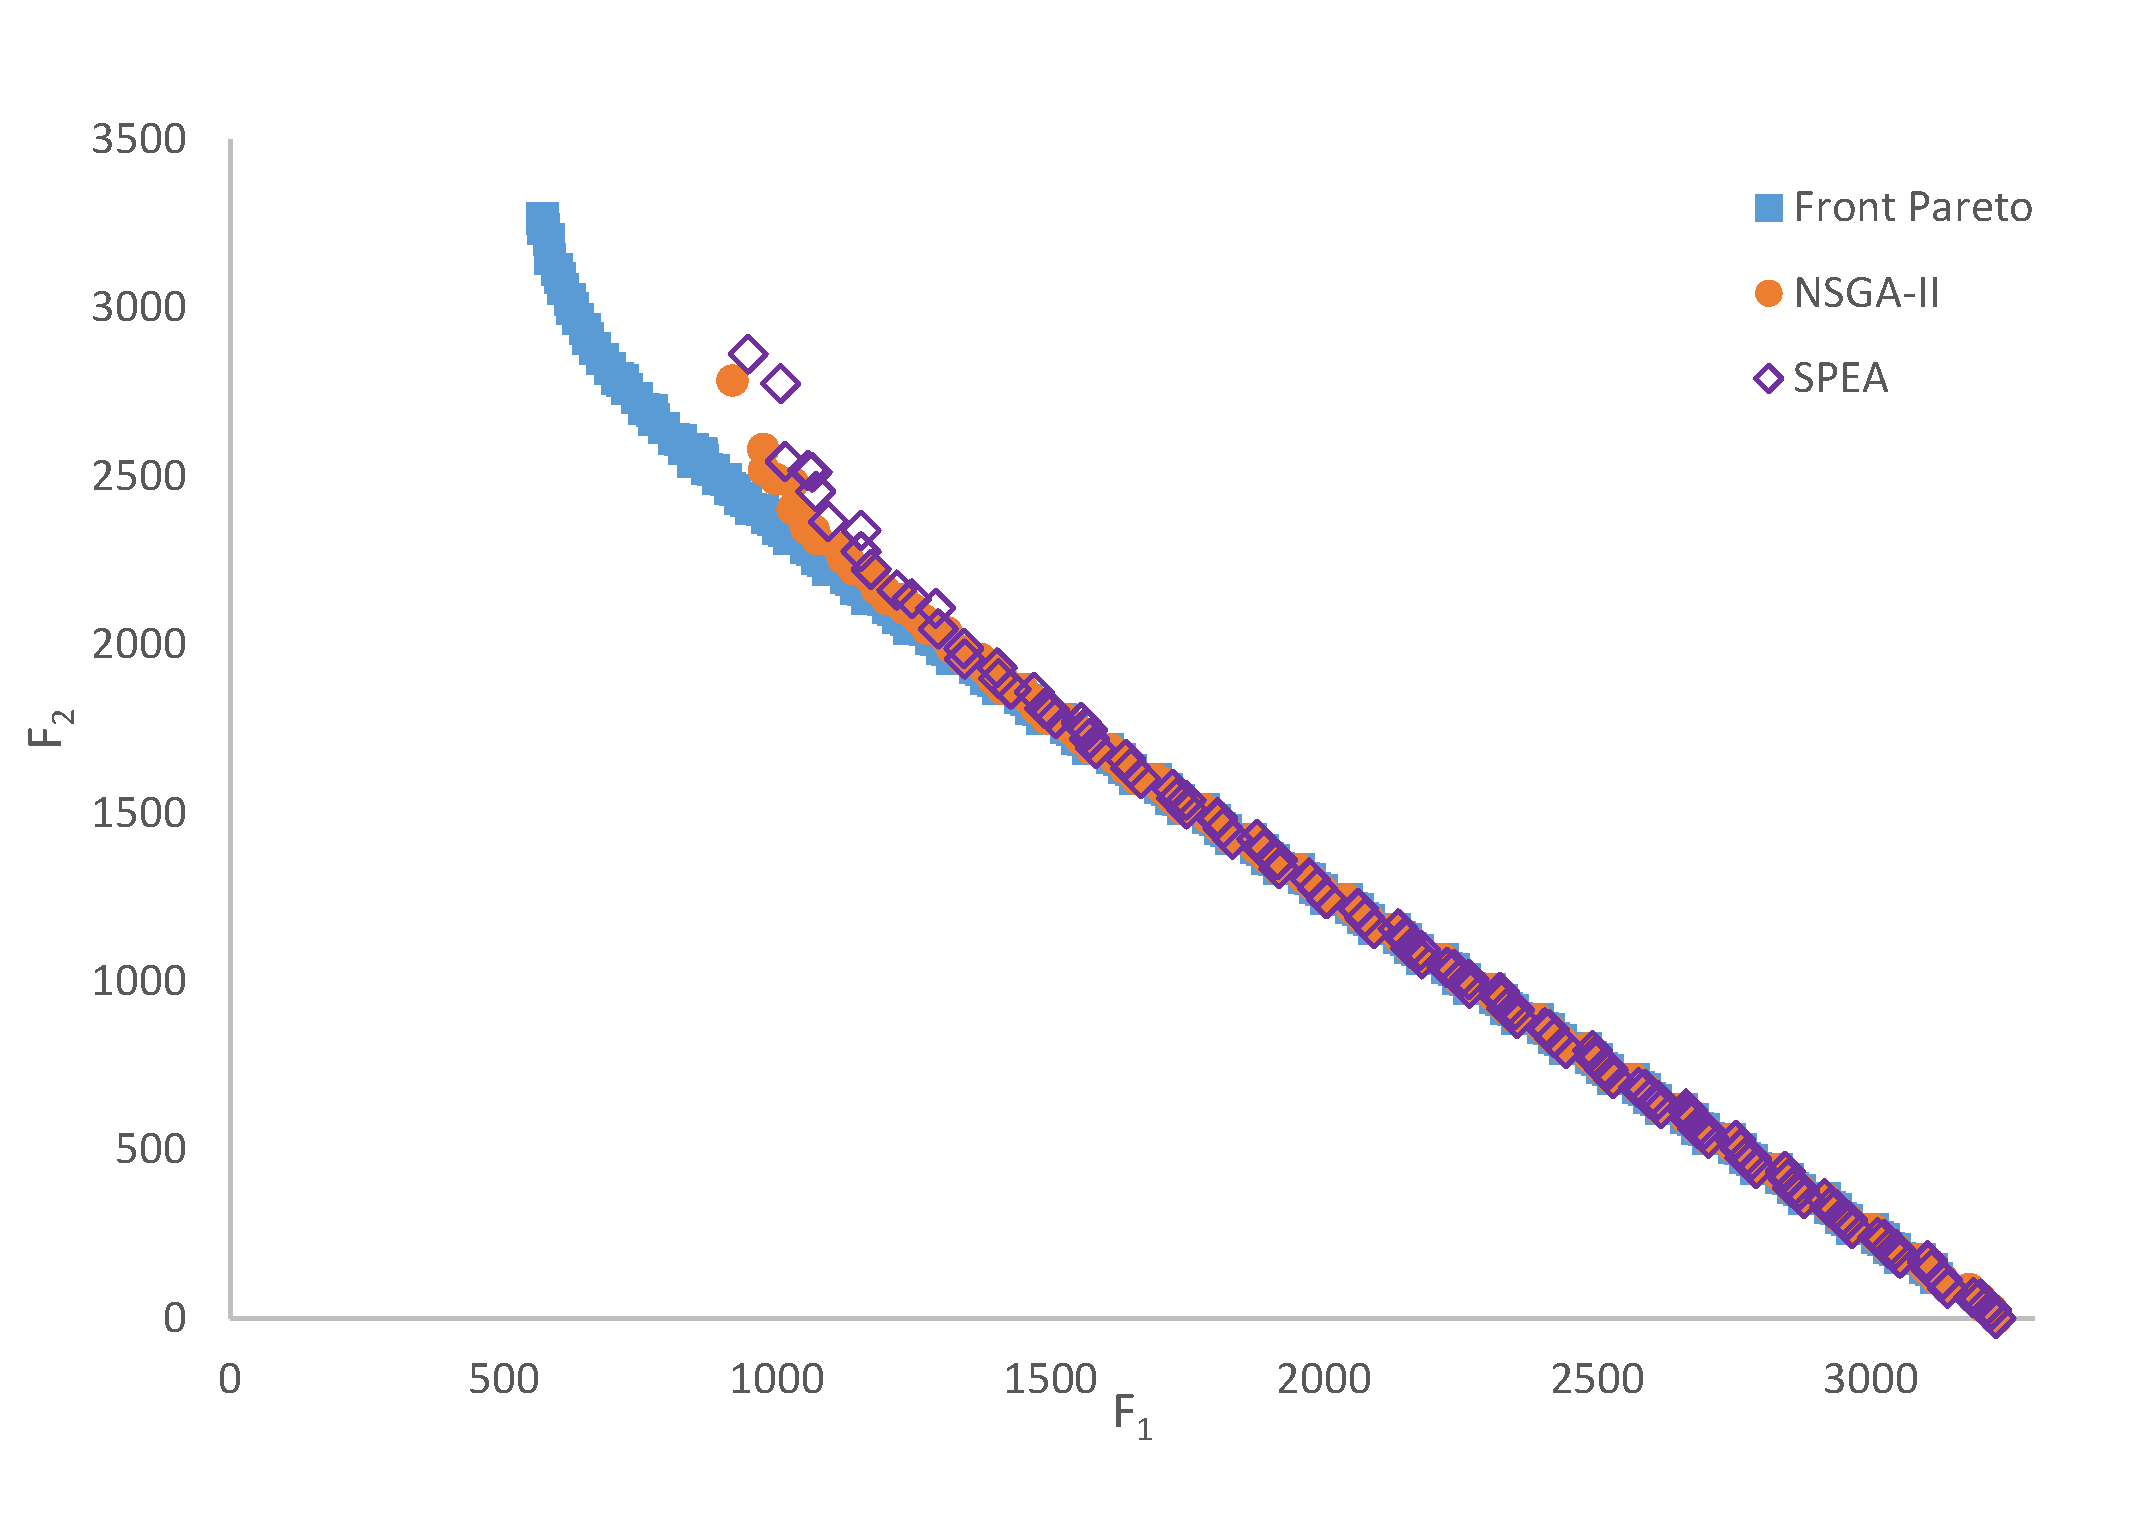
\includegraphics[width=0.5\textwidth]{big_pareto_2000}}
\subfloat[5000 generacji\label{fig:big_pareto_5000}]
        {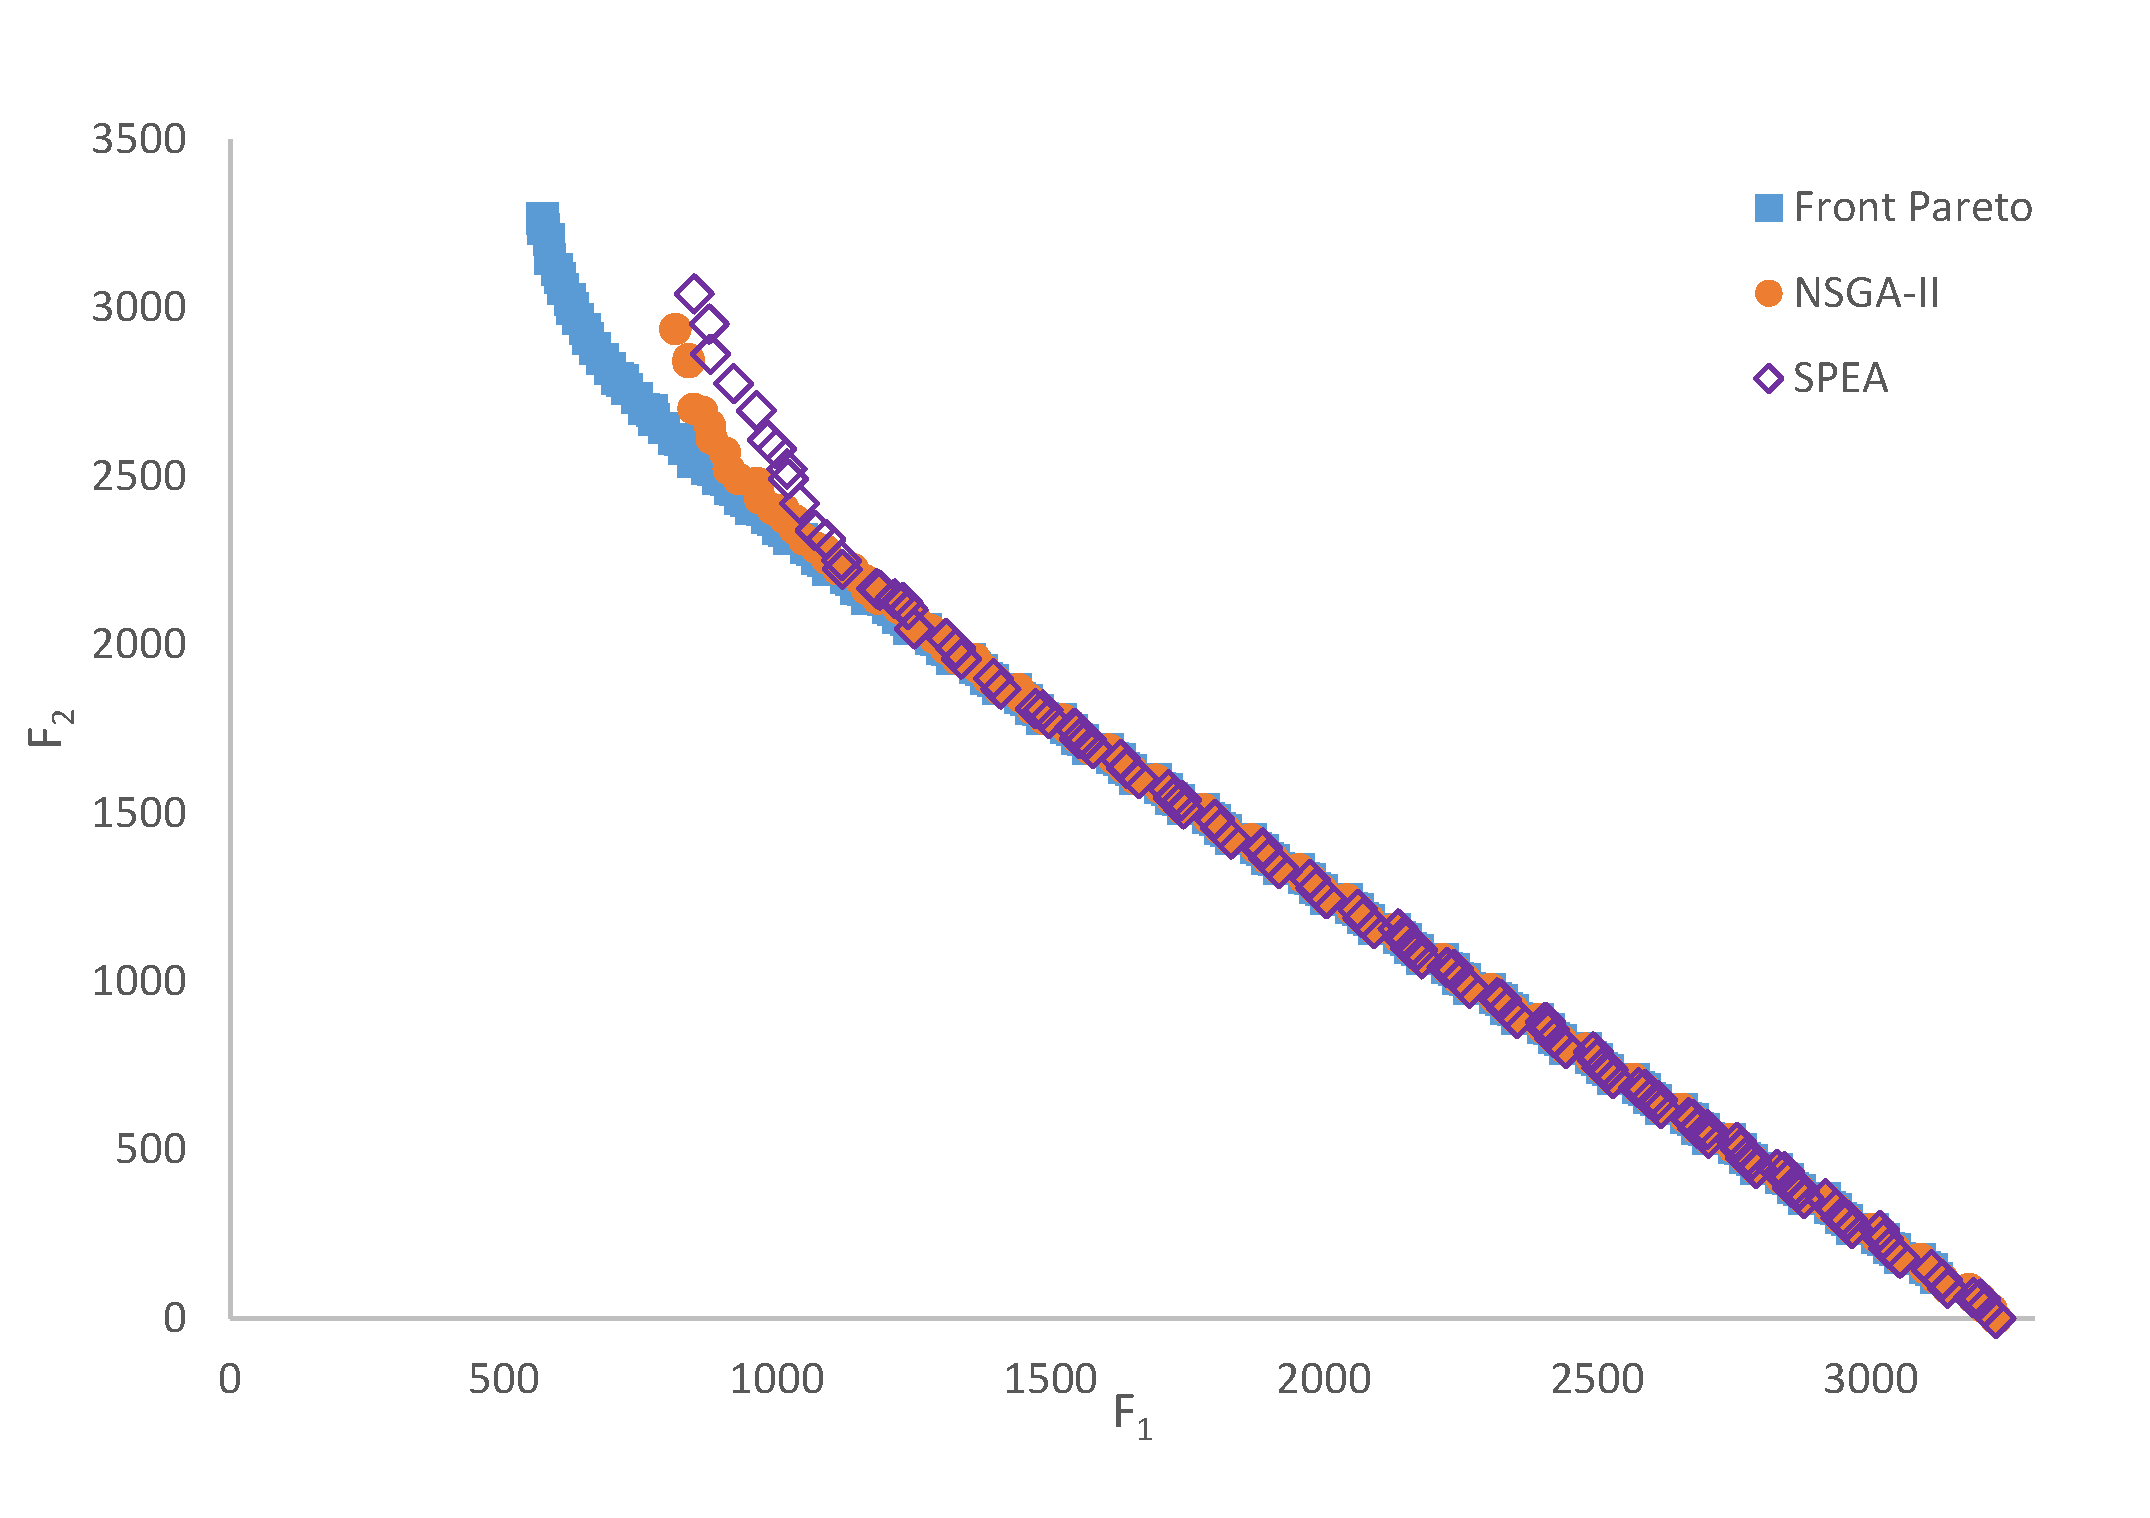
\includegraphics[width=0.5\textwidth]{big_pareto_5000}}
\caption{Rozwiązania niezdominowane otrzymane dla trzeciego przypadku testowego.}
    \label{fig:big_front}
\end{figure*}
Jak widać na przedstawionych wykresach  \eqref{fig:big_front} złożoność problemu wzrosła, co widać po zdecydowanie większym koszcie zraszaczy ($F_{2}$) potrzebnym do zminimalizowania obszaru nienawodnionego ($F_{1}$).

Podobnie jak w dwóch poprzednich przypadkach algorytmy nie miały problemu ze znalezieniem rozwiązań optymalnych wykorzystujących małą liczbę zraszaczy. Nie mniej jednak już od 100. pokolenia można zauważyć przewagę algorytmu NSGA-II \eqref{fig:big_metrics}, który znalazł rozwiązania charakteryzujące się lepszymi wartościami dla wszystkich zdefiniowanych metryk.
\begin{figure*}\centering
\subfloat[Współczynnik błędu (ER)\label{fig:er_big}]
        {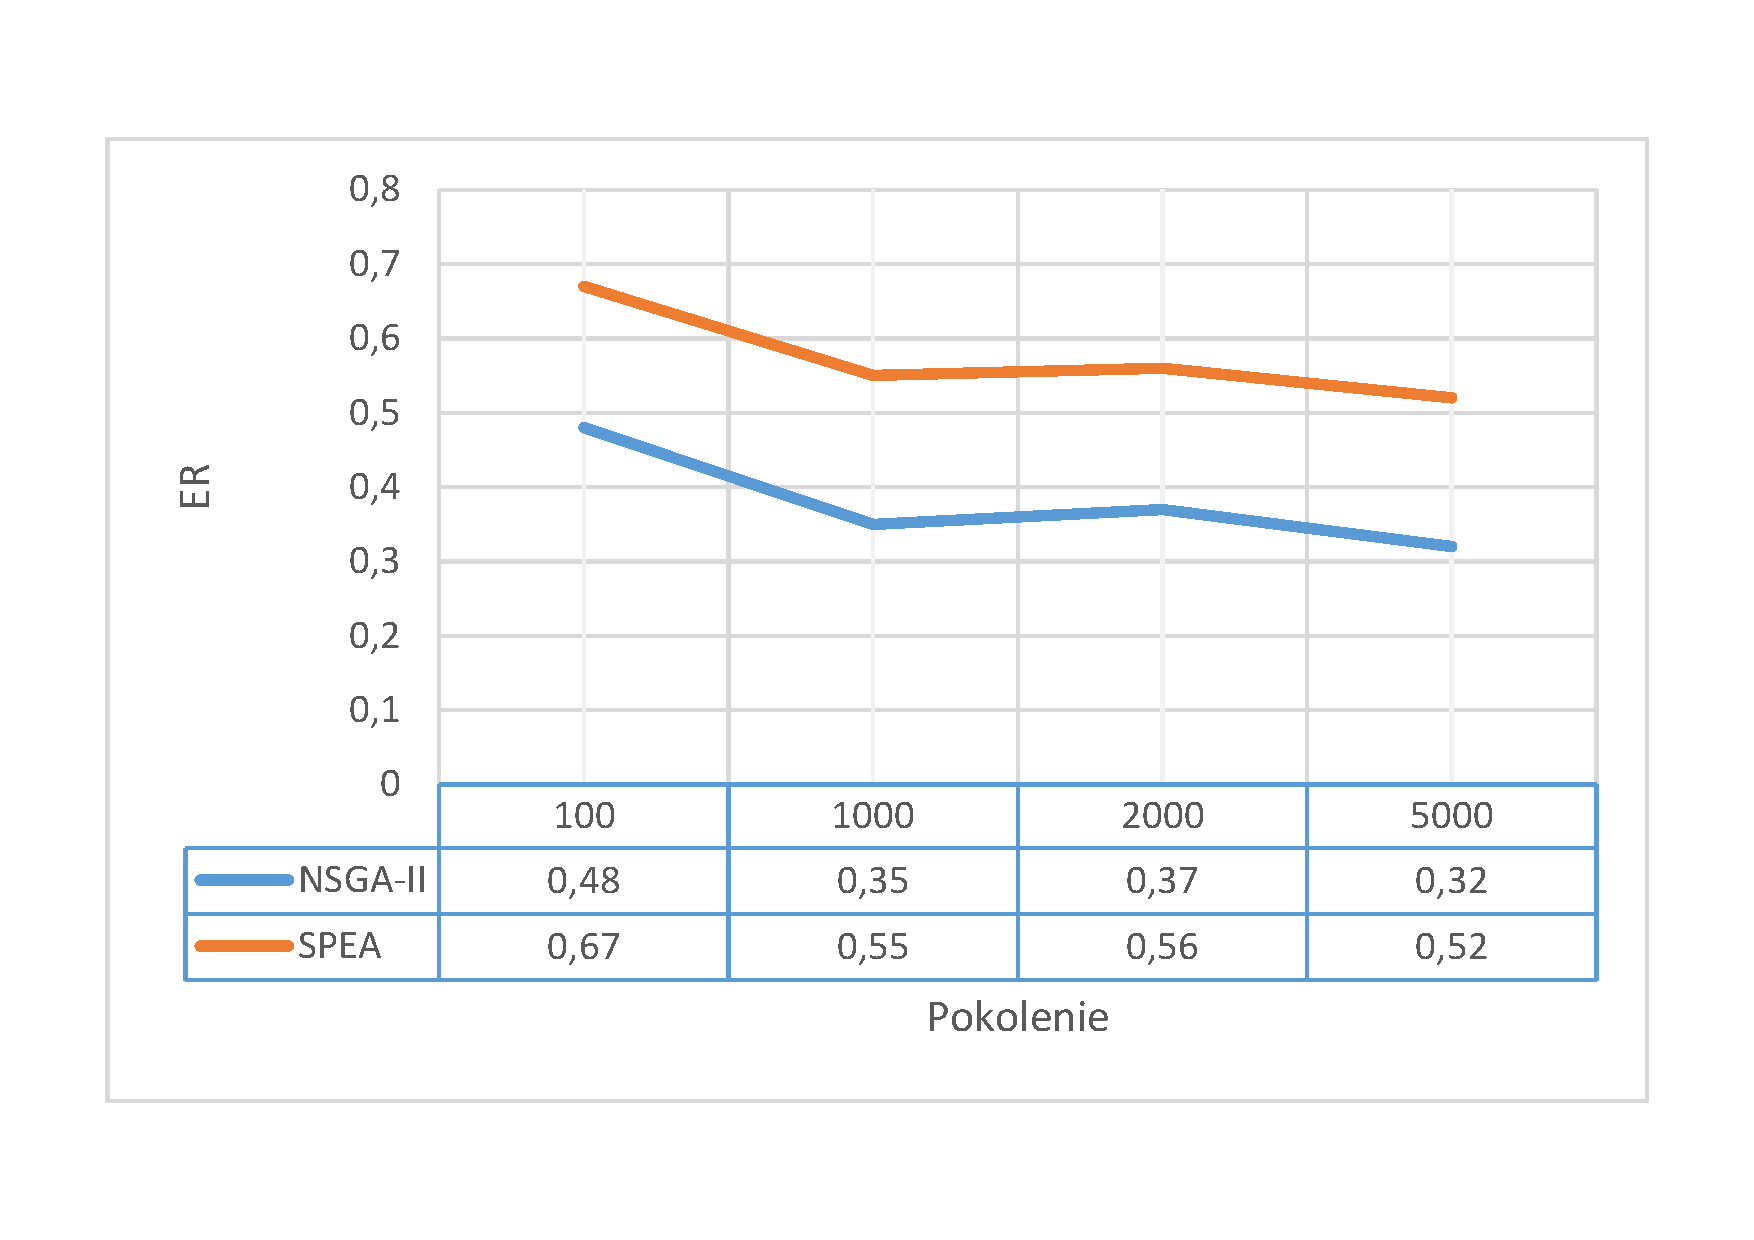
\includegraphics[width=0.5\textwidth]{er_big}}
    \hfill
\subfloat[Długość frontu (FE)\label{fig:fe_big}]
         {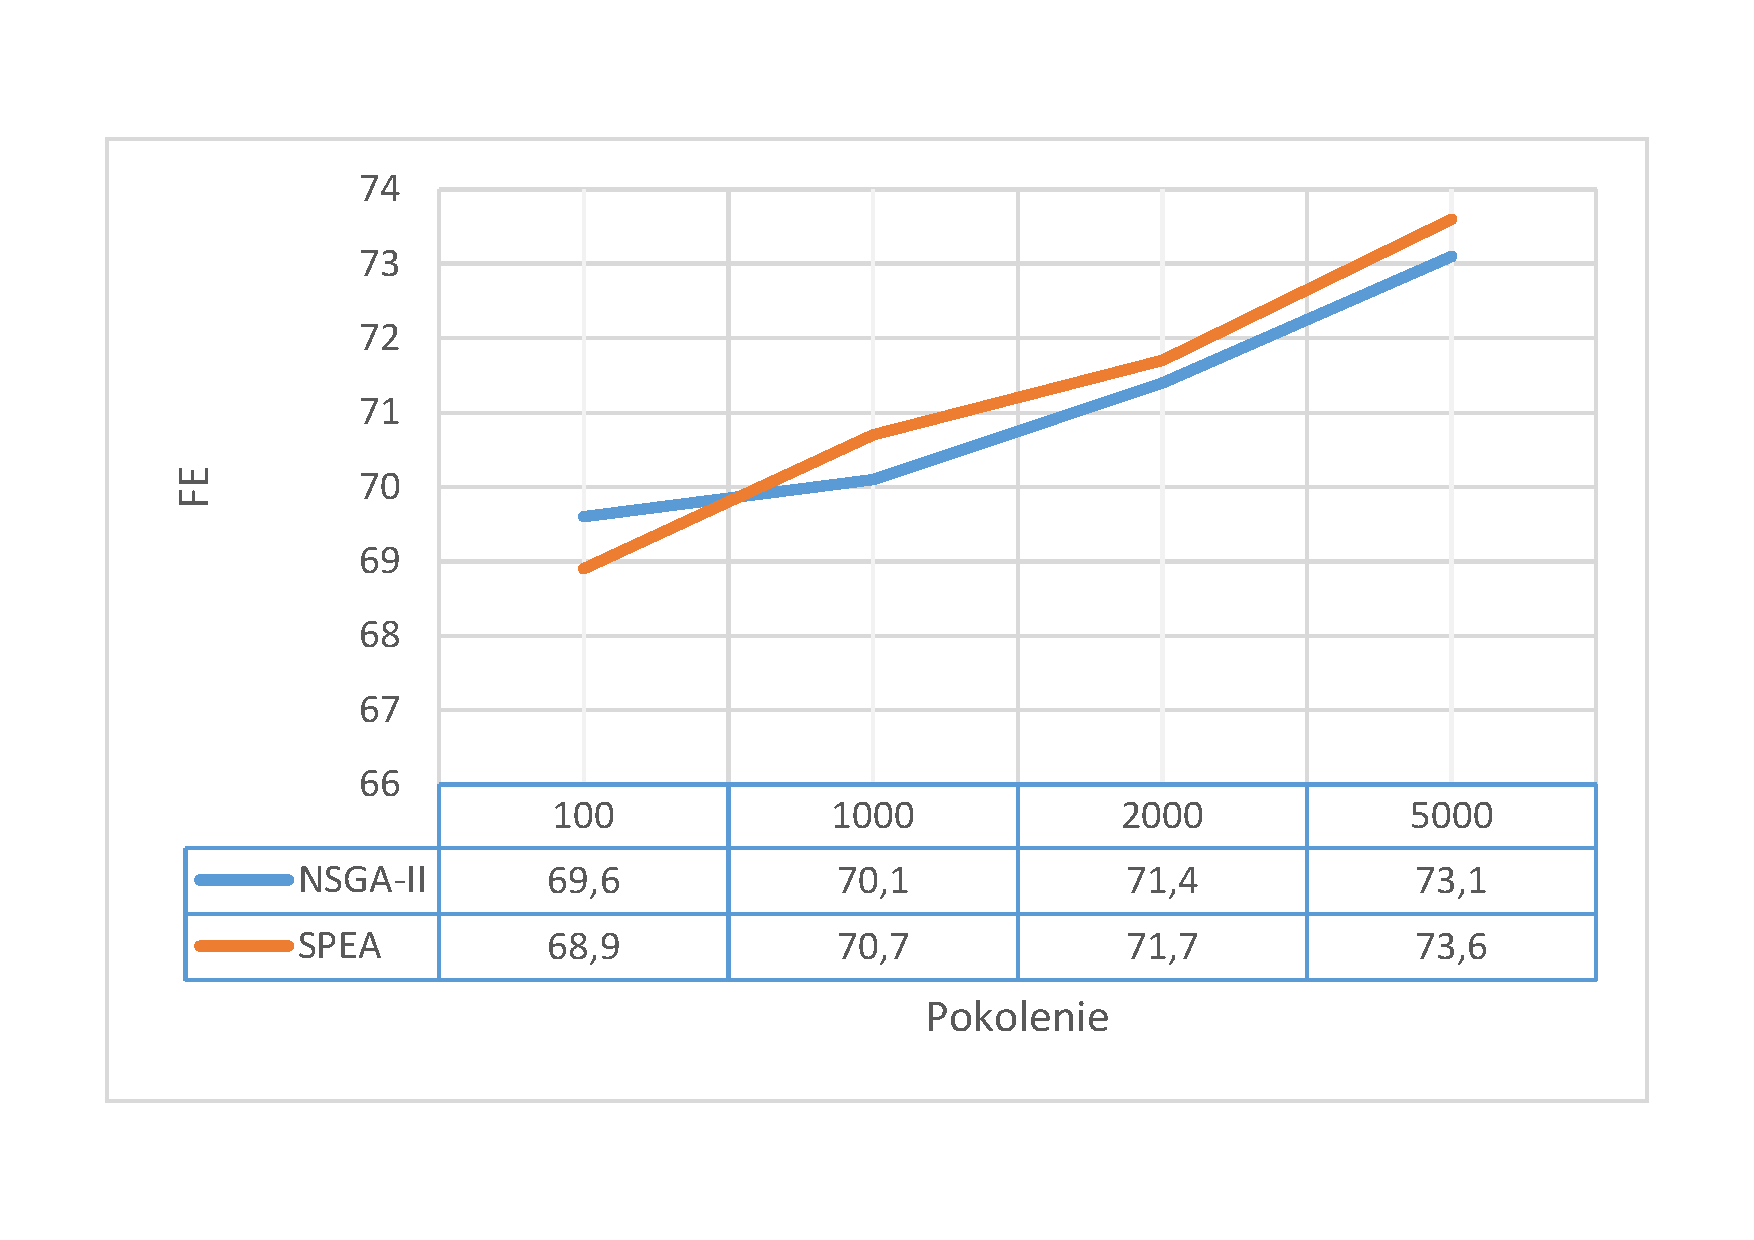
\includegraphics[width=0.5\textwidth]{fe_big}}

\subfloat[Jakość ogólna (GD)\label{fig:gd_big}]
         {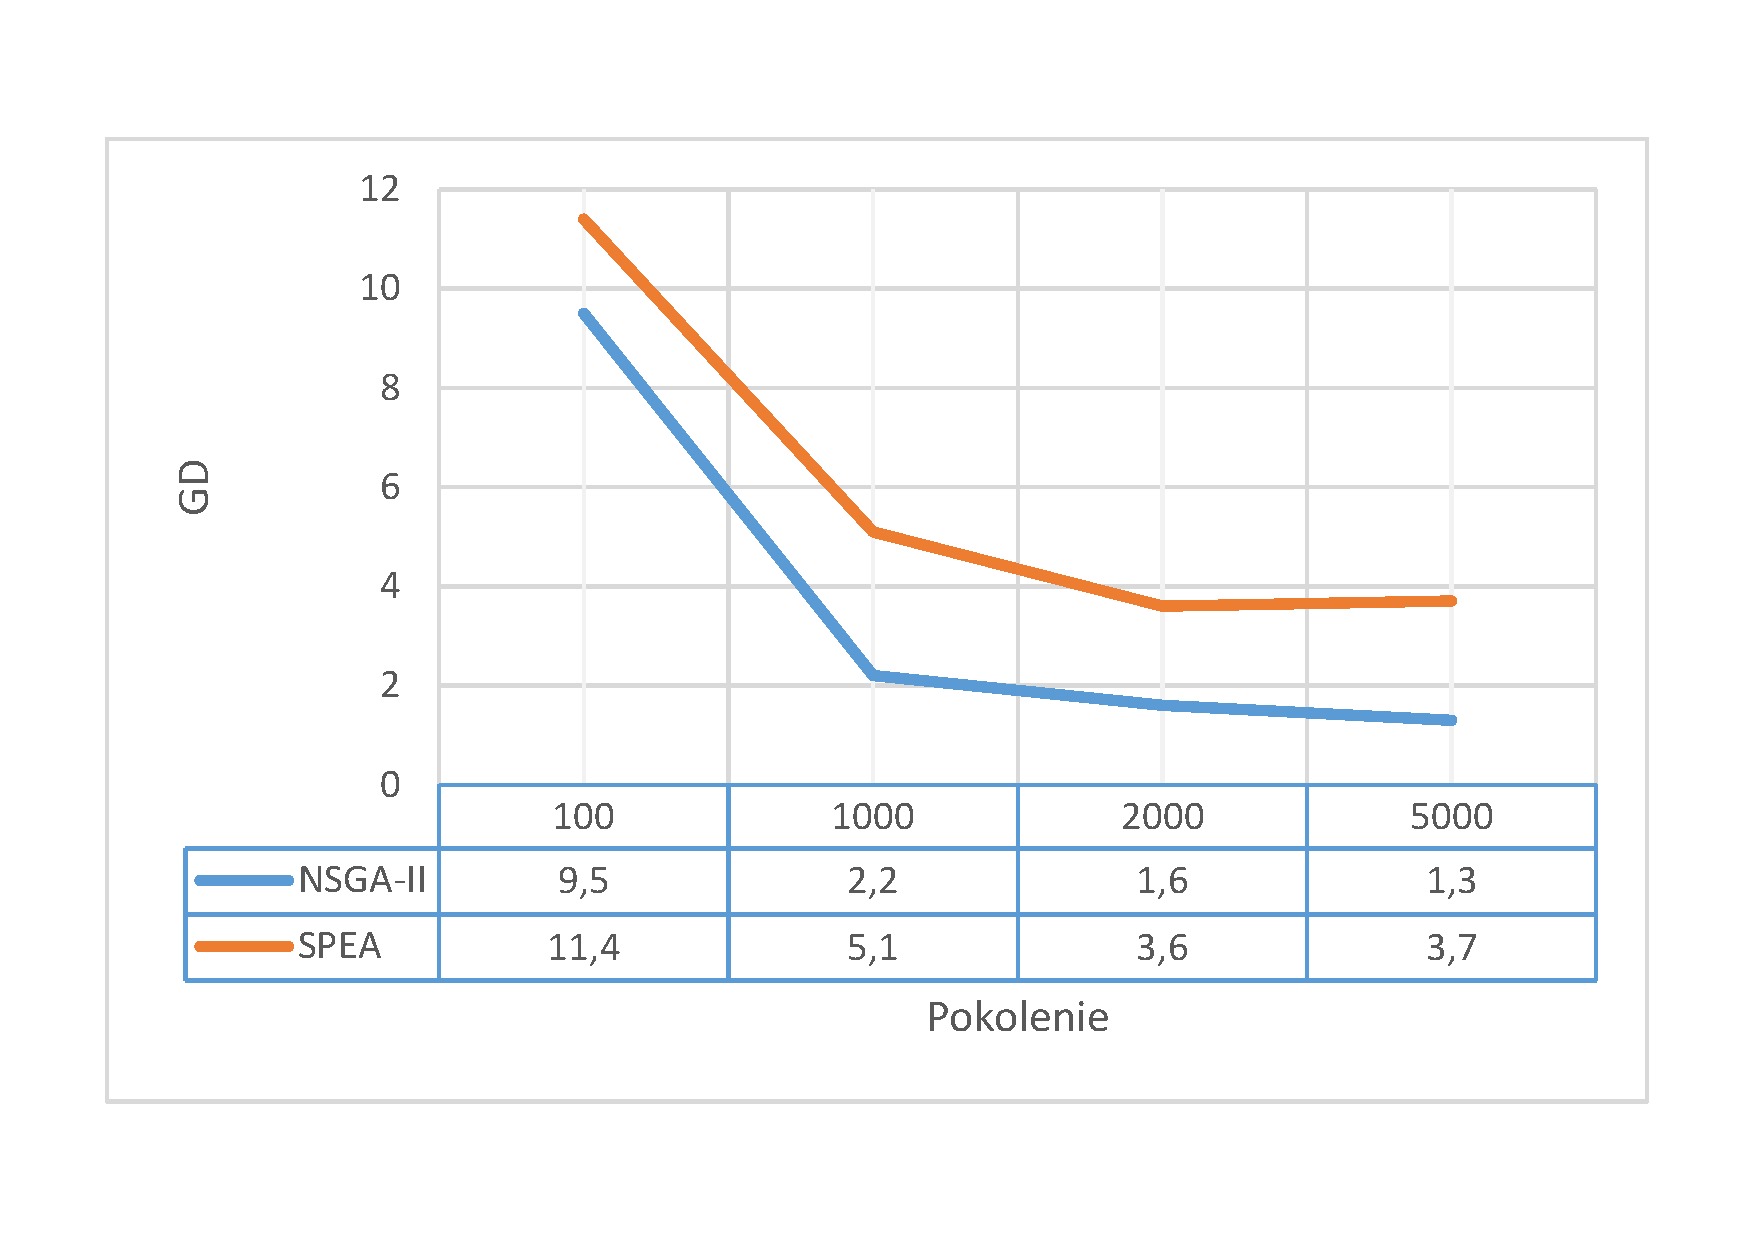
\includegraphics[width=0.5\textwidth]{gd_big}}
    \hfill
\subfloat[Równomierność rozkładu (SP)\label{fig:sp_big}]
        {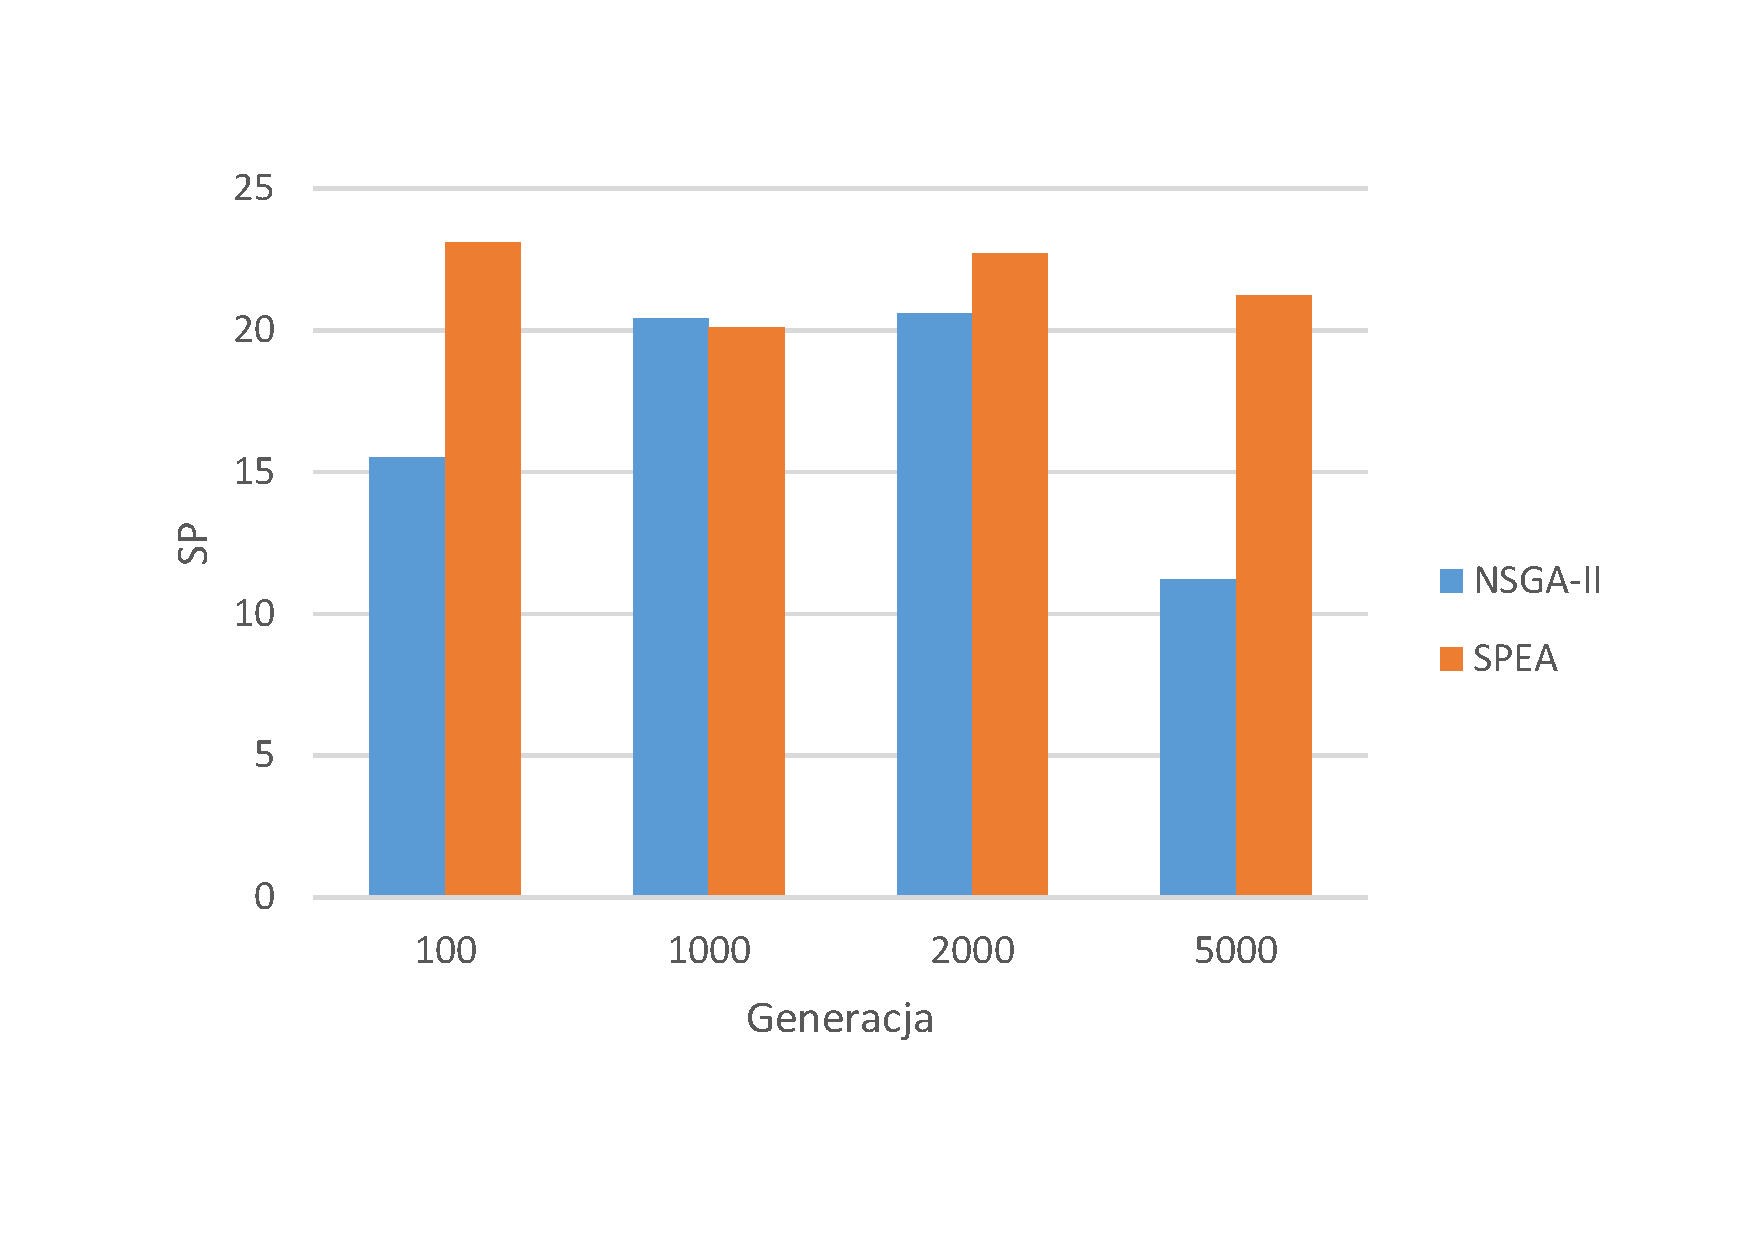
\includegraphics[width=0.5\textwidth]{sp_big}}
\caption{Wartość metryk charakteryzujących wyniki symulacji dla trzeciego przypadku testowego.}
    \label{fig:big_metrics}
\end{figure*}
W kolejnych pokoleniach sytuacja zmienia się jedynie dla metryki oceniającej długość wygenerowanego frontu. W tym przypadku lepiej wypada algorytm SPEA.

Podsumowując, podobnie jak w drugim przypadku testowym, algorytm NSGA-II wypadł lepiej od algorytmu SPEA. Patrząc na wykresy \eqref{fig:big_front} łatwo zauważyć zdecydowaną przewagę, na którą składają się rozwiązania znajdujące się bliżej frontu Pareto, mniejszy współczynnik błędu ($ER$) oraz lepsza równomierność rozkładu znalezionych rozwiązań. Algorytm SPEA charakteryzuje się jedynie generacją dłuższego frontu, co nie ma większego znaczenia w kontekście wyboru lepszego algorytmu.

\subsubsection{Czas działania}
Poza oceną algorytmów przy wykorzystaniu opisanych wcześniej metryk zdecydowano się również na sprawdzenie złożoności czasowej. Rezultaty zostały przedstawione na wykresie \eqref{fig:time}. Badanie wykonano na drugim przypadku testowym (obszar średni) dla 5000 generacji. Jak widać algorytm SPEA zakończył symulację niemal o połowę szybciej w porównaniu do NSGA-II. Z tego względu zdecydowano się rozszerzyć proces badawczy o dodatkową symulację sprawdzającą jakość zastosowanych algorytmów w zależności od czasu.
\begin{figure}[H]
	\makebox[\textwidth]{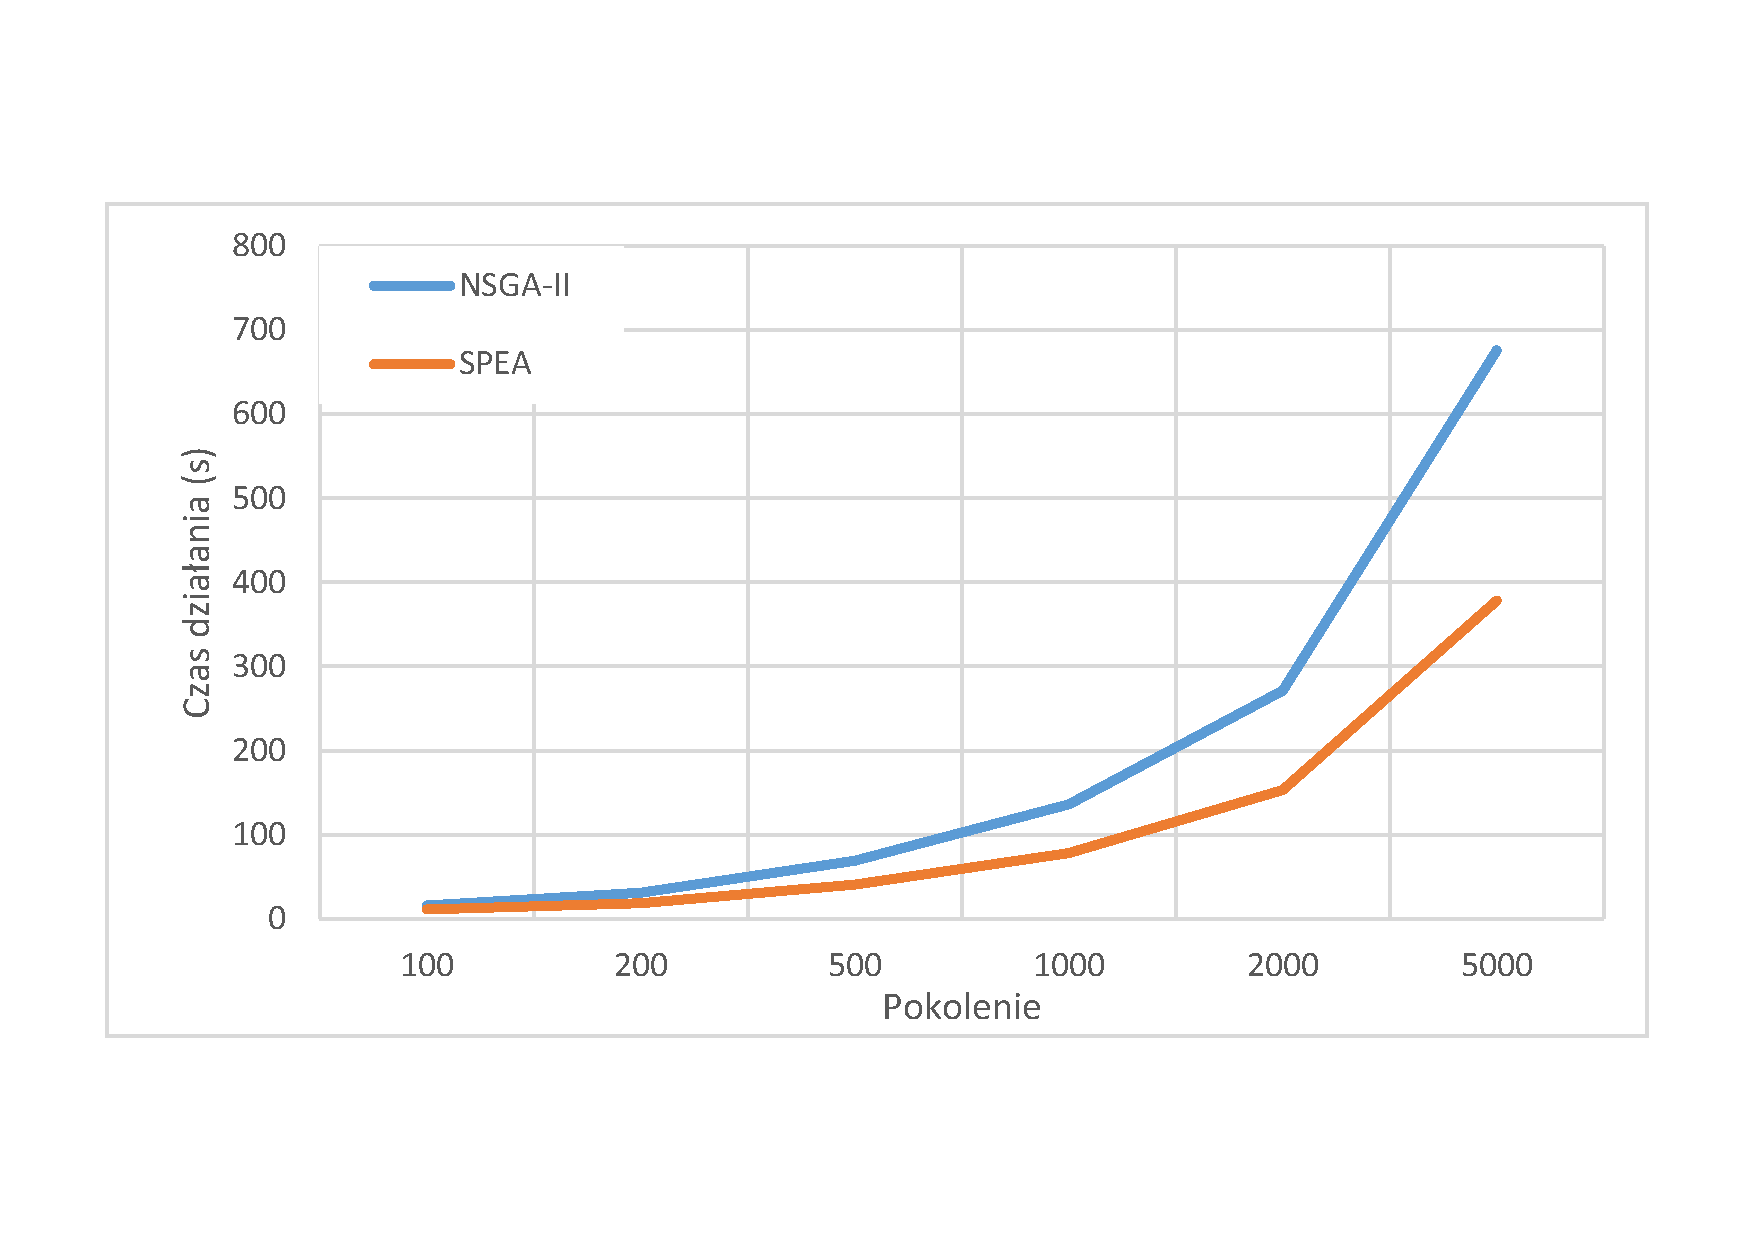
\includegraphics[ clip, scale=0.5]{time}}
	\centering
	\caption{Czasy potrzebne do wykonania symulacji}
	\label{fig:time}
\end{figure}
Pod uwagę wzięto trzeci przypadek testowy. Oba algorytmy pracowały przez godzinę. Na wykresach \eqref{fig:big_time_results} przedstawione zostały rezultaty przeprowadzonej symulacji
\begin{figure*}\centering
\subfloat[10 minut\label{fig:big_time_10}]
        {\includegraphics[width=0.5\textwidth]{big_time_10}}
    \hfill
\subfloat[20 minut\label{fig:big_time_20}]
         {\includegraphics[width=0.5\textwidth]{big_time_20}}

\subfloat[30 minut\label{fig:big_time_30}]
         {\includegraphics[width=0.5\textwidth]{big_time_30}}
    \hfill
\subfloat[40 minut\label{fig:big_time_40}]
        {\includegraphics[width=0.5\textwidth]{big_time_40}}
    \hfill
\subfloat[50 minut\label{fig:big_time_50}]
        {\includegraphics[width=0.5\textwidth]{big_time_50}}
    \hfill
\subfloat[60 minut\label{fig:big_time_60}]
        {\includegraphics[width=0.5\textwidth]{big_time_60}}
\caption{Rozwiązania niezdominowane otrzymane dla trzeciego przypadku testowego po określonym czasie.}
    \label{fig:big_time_results}
\end{figure*}
Po ocenie złożoności czasowej algorytmów, można było mieć nadzieję, że wyniki wygenerowane przez SPEA w wyniku dodatkowej symulacji będą lepsze od tych znalezionych przez algorytm NSGA-II. Sprawiałoby to, że SPEA stałby się atrakcyjniejszym wyborem w kontekście zastosowania w opracowanym systemie wspomagania decyzji. Stałoby się tak, ponieważ dla użytkownika większe znaczenie ma który algorytm w stosunkowo krótkim czasie zwróci lepsze rezultaty, a nie to jak te rezultaty będą wyglądać po ewaluacji 5000 pokoleń.
Jak widać na zamieszczonych wykresach oraz tabelach prezentujących poszczególne metryki \eqref{fig:big_time_metrics} powyższy scenariusz nie sprawdził się. Ponownie lepszym wyborem okazuje się algorytm NSGA-II. Przez cały czas trwania symulacji wyniki generowane przez NSGA-II charakteryzowały się mniejszym współczynnikiem błędu, były rozłożone na dłuższym froncie oraz co najważniejsze, po 60 minutach pracy wszystkie rozwiązania leżały na froncie Pareto, na co wskazuje metryka $GD$. Ponadto cechowały się lepszą równomiernością rozkładu.
\begin{figure*}\centering
\subfloat[Współczynnik błędu (ER)\label{fig:times_er}]
        {\includegraphics[width=0.5\textwidth]{times_er}}
    \hfill
\subfloat[Długość frontu (FE)\label{fig:times_fe}]
         {\includegraphics[width=0.5\textwidth]{times_fe}}

\subfloat[Jakość ogólna (GD)\label{fig:times_gd}]
         {\includegraphics[width=0.5\textwidth]{times_gd}}
    \hfill
\subfloat[Równomierność rozkładu (SP)\label{fig:times_sp}]
        {\includegraphics[width=0.5\textwidth]{times_sp}}
\caption{Wartość metryk charakteryzujących wyniki symulacji dla trzeciego przypadku testowego po określonym czasie.}
    \label{fig:big_time_metrics}
\end{figure*}
\subsection{Podsumowanie badań}
Po analizie rezultatów przeprowadzonych badań jednoznacznie okazało się, że lepszym wyborem przy rozwiązywaniu zdefiniowanego w pracy problemu jest algorytm NSGA-II. We wszystkich przypadkach testowych radził sobie lepiej lub równie dobrze co algorytm SPEA.

Pierwszy przypadek testowy reprezentował najprostszy scenariusz. Algorytmy miały za zadanie rozwiązać problem optymalizacyjny na małym obszarze roboczym, przez co złożoność problemu była zdecydowanie mniejsza w porównaniu do kolejnych przypadków. Oba algorytmy w stosunkowo krótkim czasie znalazły rozwiązania leżące na froncie Pareto lub w jego bliskim sąsiedztwie. Rozwiązania znalezione przez NSGA-II cechowały się lepszą jakością ogólną, równomiernością rozkładu oraz rozciągały się na dłuższym froncie. Rozwiązania algorytmu SPEA charakteryzowały się natomiast mniejszym współczynnikiem błędu. Jak widać algorytm NSGA-II okazał się lepszy w kontekście trzech metryk na cztery. Należy tutaj jednak zwrócić uwagę, że różnice pomiędzy algorytmami dla małego obszaru nie były tak znaczące jak w pozostałych przypadkach. Co więcej jak wykazało badanie złożoności czasowej algorytm SPEA potrzebuje niemal o połowę czasu mniej na ewaluację 1000 generacji. Biorąc to pod uwagę, dla problemów opartych na małym obszarze kiedy algorytmy nie mają problemów ze znalezieniem dobrych rozwiązań, lepszym wyborem może okazać się algorytm SPEA, właśnie ze względu na czas działania oraz porównywalną do NSGA-II jakość znalezionych rozwiązań.

Dla drugiego przypadku testowego został wybrany obszar mający reprezentować scenariusz o średnim stopniu trudności. Jak widać po załączonych wykresach oraz tabelach wraz ze wzrostem złożoności problemu rośnie przewaga algorytmu NSGA-II. Rozwiązania znajdowane w poszczególnych pokoleniach przez NSGA-II znajdowały się zdecydowanie bliżej frontu Pareto oraz cechowały się lepszą równomiernością rozkładu. Co prawda SPEA wygenerował rozwiązania rozciągające się na dłuższym froncie, a więc w praktyce zapewniające większą różnorodność. Należy jednak zwrócić tutaj uwagę, że jedynie rozwiązania znalezione dla małych wartości funkcji $F_{2}$ są równie dobre co odpowiedniki znalezione przez NSGA-II. Dla większych wartości $F_{2}$ ($> 800$), wszystkie rozwiązania SPEA są zdominowane przez rozwiązania NSGA-II.

Ostatni przypadek testowy był reprezentowany przez największy obszar. W tym przypadku żadnemu algorytmowi przez 5000 generacji nie udało się znaleźć rozwiązań rozciągających się na całej długości frontu Pareto. Podobnie jak w poprzednim przypadku dłuższy front wygenerował algorytm SPEA. Nie przekłada się to jednak na ogólną jakość rozwiązań. NSGA-II znalazł rozwiązania cechujące się lepszym wartościami dla wszystkich pozostałych metryk.

Po porównaniu algorytmów w kontekście różnych przypadków testowych zdecydowano się dodatkowo na zbadanie ich złożoności czasowej. Badanie wykonano dla drugiego przypadku testowego. Jednoznacznym zwycięzcą porównania okazał się algorytm SPEA, który zakończył ewaluację 5000 pokoleń w czasie o połowę krótszym od algorytmu NSGA-II.

Biorąc pod uwagę poprzednie wyniki oraz te obrazujące czas działania zdecydowano się sprawdzić czy SPEA jest w stanie wygenerować równie dobre wyniki co NSGA-II, biorąc pod uwagę, nie liczbę populacji, lecz złożoność czasową. Metryka taka jest bowiem bardziej naturalnym wyborem jeśli chodzi o systemy wspomagania decyzji. Użytkownika bowiem nie będzie obchodziło po ilu generacjach dany algorytm znalazł rozwiązania leżące na froncie Pareto, lecz jak szybko udało się to zrobić.

Dodatkową symulację przeprowadzona na trzecim przypadku testowym. Jak się okazało mimo mniejszej złożoności czasowej algorytm SPEA przez godzinę pracy nie był w stanie wygenerować rozwiązań lepszych niż NSGA-II. Co więcej po 60 minutowej symulacji wszystkie rozwiązania znalezione przez NSGA-II znajdowały się na froncie Pareto, co dobrze obrazują metryki: $ER=0$ oraz $GD=0$.

Podsumowując, lepszym wyborem przy rozwiązywaniu zdefiniowanego w pracy problemu jest algorytm NSGA-II co zostało udowodnione poprzez rezultaty badań oraz powyższe podsumowanie.
\chapter{Podsumowanie}
Celem pracy było opracowanie systemu wspomagającego podejmowanie decyzji w rozmieszczeniu zraszaczy wodnych oraz połączeń między nimi na zadanej powierzchni oraz wybór i porównanie wielokryterialnych algorytmów genetycznych w kontekście zdefiniowanego problemu.

Powyższe cele zostały zrealizowane. Jako rezultat pracy powstał system wspomagania decyzji w formie aplikacji webowej znacznie ułatwiający proces projektowania systemu nawadniania ogrodu. Użytkownik poprzez zaimplementowaną aplikację może w prosty sposób zdefiniować obszar mający zostać nawodniony oraz otrzymać kilka wariantów rozwiązania w czytelnej i przejrzystej formie.

Ponadto wybrano oraz porównano ze sobą dwa wielokryterialne algorytmy genetyczne. Do badań wykorzystano trzy przypadki testowe oraz zdefiniowano cztery metryki pomagające w ocenie wygenerowanych przez algorytmy rozwiązań. Z przeprowadzonych badań wynika, że dla problemów reprezentowanych przez stosunkowo małe obszary równie dobrze spisują się oba algorytmy. Biorąc jednak pod uwagę ich złożoność czasową, lepszą opcją w przypadku takich problemów może okazać się algorytm SPEA, który charakteryzuje się szybszym działaniem. W trudniejszych przypadków testowych zdecydowanie lepiej wypada algorytm NSGA-II, którego rozwiązania cechują się lepszymi wartościami dla wszystkich zdefiniowanych metryk.

biorąc pod uwagę wyniki przeprowadzonych badań w opracowanym systemie wspomagania decyzji zdecydowano się na wykorzystanie algorytmu NSGA-II.

Rozmieszczenie rur pomiędzy zraszaczami nie wchodziło w zakres pracy wybranych algorytmów genetycznych. Schemat połączeń był generowany dla każdego znalezionego rozwiązania za pomocą algorytmu Prima znajdującego minimalne drzewo rozpinające grafu.

Podsumowując wszystkie założone cele pracy zostały zrealizowane.\\

W kolejnych pracach zajmujących się podobnymi zagadnieniami autorzy powinni skupić się porównaniu algorytmów genetycznych z innymi metodami służącymi do optymalizacji wielokryterialnej. Szczególnie w kontekście systemów wspomagania decyzji. Jak zostało przedstawione w badaniach wybrane algorytmy dobrze radzą sobie z rozmieszczeniem zraszaczy, aczkolwiek charakteryzują się dużą złożonością czasową - dla trzeciego przypadku testowego algorytm NGSA-II osiągnął front Pareto po godzinie pracy. Dla użytkownika może to okazać się czasem za długim. 

Jeśli natomiast wybrane w pracy algorytmy genetyczne w porównaniu z innymi metodami wypadną zdecydowanie lepiej, warto byłoby zastanowić się nad porównaniem NSGA-II oraz SPEA z innymi algorytmami genetycznymi, które być może będą cechować się znajdowaniem lepszych lub równie dobrych rozwiązań oraz mniejszą złożonością czasową.

Ze względu na długi czas oczekiwania na rezultaty być może warto by zastanowić się nad zmianą formy prezentacji wyników. W obecnie opracowanym systemie wyniki prezentowane są bezpośrednio na stronie, a więc użytkownik zmuszony jest na nie czekać. Warto by zastanowić się czy lepszym rozwiązaniem nie byłoby chociażby wysyłanie pliku z wynikami w formacie PDF na adres e-mail podany przez użytkownika. Takie rozwiązanie w jakimś stopniu zwalnia użytkownika z konieczności przebywania na stronie aż do zwrócenia przez serwer rezultatów. Aczkolwiek plik PDF nie zapewnia żadnej formy interaktywności, która w takich systemach powinna być obecna.

Rozwiązaniem łączącym oba podejścia może być wysyłanie na maila użytkownika odnośnika do strony zawierającej wygenerowane rozwiązania.

Kolejnym elementem wartym modyfikacji jest zdefiniowanie bardziej dokładnego modelu matematycznego. W tym momencie brane są pod uwagę jedynie zraszacze dookolne co nakłada dodatkowe ograniczenia na znalezione rozwiązania. Przykładem jest chociażby fakt, że dany obszar nie może zostać w 100\% nawodniony bez naruszenia ograniczeń mówiących o nie podlewaniu obszaru poza tym wyznaczonym przez użytkownika. Problem ten może zostać zlikwidowany poprzez dodanie dodatkowych cech do rozmieszczonych zraszaczy, takich jak kąt rozrzutu wody oraz kierunek rozrzutu.

Ostatnim elementem wartym dokładniejszego przeanalizowania jest rozmieszczenie rur pomiędzy zraszaczami. W tej pracy wykorzystano prosty algorytm Prima, aby rozwiązać ten problem. Kolejne publikację skupiające się na podobnych problemach powinny zastosować dokładniejsze podejście. Po pierwsze pod uwagę należy wziąć ciśnienie wody, a co za tym idzie średnicę rur. Po drugie do całościowego kosztu wygenerowanego rozwiązania należy doliczyć połączenia pomiędzy zraszaczami oraz dodatkowe elementy potrzebne do instalacji tych połączeń, jak np. rozgałęźniki, kolanka itp.
%\bibliographystyle{apalike}%Used BibTeX style is unsrt

\bibliographystyle{iisthesis}
\bibliography{bibliography}

\end{document}

